\documentclass[12pt]{article}
\usepackage{amsmath}
\usepackage{graphicx}
\usepackage{enumerate}
\usepackage{natbib}
\usepackage{url} % not crucial - just used below for the URL 
\usepackage{chngcntr}
\usepackage{multirow}
\usepackage{longtable}
\usepackage{lscape}
\usepackage{rotating}

%\pdfminorversion=4
% NOTE: To produce blinded version, replace "0" with "1" below.
\newcommand{\blind}{0}

% DON'T change margins - should be 1 inch all around.
\addtolength{\oddsidemargin}{-.5in}%
\addtolength{\evensidemargin}{-1in}%
\addtolength{\textwidth}{1in}%
\addtolength{\textheight}{1.7in}%
\addtolength{\topmargin}{-1in}%

\numberwithin{equation}{section}
\numberwithin{table}{section}

\RequirePackage[OT1]{fontenc}
\usepackage{amsthm,amsfonts,amssymb,mathtools,tikz}
\usepackage{graphicx,bm,environ}
\usepackage{mathabx}
\usepackage{float}
\usepackage[boxed, linesnumbered,ruled,lined,commentsnumbered]{algorithm2e}
\RequirePackage{natbib}
\usepackage{xr-hyper}
\RequirePackage[colorlinks,citecolor=blue,urlcolor=blue]{hyperref}
\usepackage[nameinlink]{cleveref}

% provide arXiv number if available:
%\arxiv{2101.07776}

% put your definitions there:
\newcommand{\R}{\mathbb{R}}
\newcommand{\C}{\mathbb{C}}
\newcommand{\N}{\mathbb{N}}
\newcommand{\E}{\mathbb{E}}
\newtheorem{ass}{Assumption}
\newcommand{\assautorefname}{Assumption}
\newtheorem{thm}{Theorem}
\numberwithin{thm}{section}
\newcommand{\thmautorefname}{Theorem}
\newtheorem{defn}{Definition}
\numberwithin{defn}{section}
\newcommand{\defnautorefname}{Definition}
\newtheorem{lem}{Lemma}
\numberwithin{lem}{section}
\newcommand{\lemautorefname}{Lemma}
\newtheorem{prop}{Proposition}
\numberwithin{prop}{section}
\newcommand{\propautorefname}{Proposition}
\newtheorem{cor}{Corollary}
\numberwithin{cor}{section}
\newcommand{\corautorefname}{Corollary}
\newtheorem{rem}{Remark}
\numberwithin{rem}{section}
\newcommand{\remautorefname}{Remark}
\renewcommand{\sectionautorefname}{Section}
\let\subsectionautorefname\sectionautorefname 	\let\subsubsectionautorefname\sectionautorefname
\renewcommand{\algorithmautorefname}{Algorithm}
\renewcommand{\thealgocf}{B.\arabic{algocf}}

\Crefname{ass}{Assumption}{Assumptions}
\Crefname{prop}{Proposition}{Propositions}
\Crefname{section}{Section}{Sections}
\Crefname{appendix}{Appendix}{Appendices}


\DeclareMathOperator*{\argmin}{arg min}
\DeclareMathOperator*{\argmax}{arg max}
\DeclareMathOperator{\Vector}{vec}
\DeclareMathOperator{\Vech}{vech}
\DeclareMathOperator{\tr}{tr}
\DeclareMathOperator{\offvec}{offvec}
\DeclareMathOperator{\blkdiag}{blkdiag}
\DeclareMathOperator{\SNR}{SNR}
\DeclareMathOperator{\mat}{mat}
\DeclareMathOperator{\cov}{Cov}
\DeclareMathOperator{\var}{Var}
\DeclareMathOperator{\diag}{diag}
\newcommand{\rank}{\operatorname{rk}} 
%\endlocaldefs

\newenvironment{ass*}
 {\expandafter\def\expandafter\theass\expandafter{\theass*}\ass}
 {\endass}
%\newtheorem{assumpB}{Assumption}
%\newcommand{\assumpBautorefname}{Assumption}
%\renewcommand\theassumpB{\arabic{assumpB}^{*}}
%\Crefname{assumpB}{Assumption}{Assumptions}


%\addbibresource{main.bib}

\makeatletter
\newcommand*{\addFileDependency}[1]{% argument=file name and extension
  \typeout{(#1)}
  \@addtofilelist{#1}
  \IfFileExists{#1}{}{\typeout{No file #1.}}
}
\makeatother

\newcommand*{\myexternaldocument}[1]{%
    \externaldocument[][nocite]{#1}%
    \addFileDependency{#1.tex}%
    \addFileDependency{#1.aux}%
}

\myexternaldocument{jasa-testing_simultaneous_diagonalizability}

\begin{document}

%\bibliographystyle{natbib}

\def\spacingset#1{\renewcommand{\baselinestretch}%
{#1}\small\normalsize} \spacingset{1}


%%%%%%%%%%%%%%%%%%%%%%%%%%%%%%%%%%%%%%%%%%%%%%%%%%%%%%%%%%%%%%%%%%%%%%%%%%%%%%


  \title{\LARGE\bf Supplement to ``Testing Simultaneous Diagonalizability"}
  \author{Yuchen Xu\thanks{Corresponding author: Yuchen Xu, Email address: \href{mailto:yx439@cornell.edu}{yx439@cornell.edu}}
    \and
    Marie-Christine D\"uker\thanks{Email address: \href{mailto:md2224@cornell.edu}{md2224@cornell.edu}}
    \and
    David S. Matteson\thanks{Email address: \href{mailto:matteson@cornell.edu}{matteson@cornell.edu}}
    \hspace{.7cm}\\
    Department of Statistics and Data Science, Cornell University}
  \maketitle

We present here supplementary results for the article “Testing Simultaneous Diagonalizability”. \autoref{se:compl} provides some additional numerical results. In \autoref{sec:llrt}, we propose and analyze an alternative to the commutator based test for the two-sample test problem.
\autoref{sec:ext} discusses an extension for symmetric matrices.
Finally, \Cref{app:profs,,app:est} contain all proofs.
We adopt the notation of the article and refer to its labels.


\begin{appendix}
\counterwithin{figure}{section}

\section{Complementary simulation results} \label{se:compl}
We provide here some empirical results complementary to the numerical analysis presented in the main paper. \autoref{se:compl1} gives empirical sizes and powers for the proposed test, 
\autoref{se:compl2} studies sequential application of our partial tests and \autoref{se:compl3} discusses application to possibly high-dimensional data.

\subsection{Empirical Type I and II errors} \label{se:compl1}
In addition to the p-values in the main paper, we provide here tables with Type I and II errors for our tests to assess their performances. \Cref{ta:errorsTwosample,,ta:errorsMultisample,,ta:errorsPartial} show respectively the errors for the two-sample, multi-sample and partial tests.

\begin{table}[htbp] 
\centering
\begin{tabular}{|c|c|c|c|cc|}
\hline
\multirow{2}{*}{Test Type} & \multirow{2}{*}{\begin{tabular}[c]{@{}c@{}}Statistics\\ Type\end{tabular}} & \multirow{2}{*}{\begin{tabular}[c]{@{}c@{}}Sample\\ Size\end{tabular}} & \multirow{2}{*}{\begin{tabular}[c]{@{}c@{}}Type I\\ Error\end{tabular}} & \multicolumn{2}{c|}{Type II Error} \\ \cline{5-6} 
 &  &  &  & \multicolumn{1}{c|}{SNR=1000} & SNR=10 \\ \hline
\multirow{3}{*}{\begin{tabular}[c]{@{}c@{}}Commutator-based\\ test\end{tabular}} & \multirow{3}{*}{Chi-test} & 50 & 0.218 & \multicolumn{1}{c|}{0.216} & 0.000 \\ \cline{3-6} 
 &  & 250 & 0.056 & \multicolumn{1}{c|}{0.000} & 0.000 \\ \cline{3-6} 
 &  & 1000 & 0.054 & \multicolumn{1}{c|}{0.000} & 0.000 \\ \hline
\multirow{12}{*}{\begin{tabular}[c]{@{}c@{}}LLR test\\ (\autoref{sec:llrt})\end{tabular}} & \multirow{3}{*}{\begin{tabular}[c]{@{}c@{}}Oracle Chi-Test\\ with \eqref{eqn:polyP}\end{tabular}} & 50 & 0.182 & \multicolumn{1}{c|}{0.000} & 0.000 \\ \cline{3-6} 
 &  & 250 & 0.140 & \multicolumn{1}{c|}{0.000} & 0.000 \\ \cline{3-6} 
 &  & 1000 & 0.060 & \multicolumn{1}{c|}{0.000} & 0.000 \\ \cline{2-6} 
 & \multirow{3}{*}{\begin{tabular}[c]{@{}c@{}}Plugin Chi-test\\ with \eqref{eqn:polyP}\end{tabular}} & 50 & 1.000 & \multicolumn{1}{c|}{0.000} & 0.000 \\ \cline{3-6} 
 &  & 250 & 1.000 & \multicolumn{1}{c|}{0.000} & 0.000 \\ \cline{3-6} 
 &  & 1000 & 1.000 & \multicolumn{1}{c|}{0.000} & 0.000 \\ \cline{2-6} 
 & \multirow{3}{*}{\begin{tabular}[c]{@{}c@{}}Oracle Chi-Test\\ with \eqref{eqn:eigvP}\end{tabular}} & 50 & 0.182 & \multicolumn{1}{c|}{0.058} & 0.000 \\ \cline{3-6} 
 &  & 250 & 0.140 & \multicolumn{1}{c|}{0.000} & 0.000 \\ \cline{3-6} 
 &  & 1000 & 0.060 & \multicolumn{1}{c|}{0.000} & 0.000 \\ \cline{2-6} 
 & \multirow{3}{*}{\begin{tabular}[c]{@{}c@{}}Plugin Chi-test\\ with \eqref{eqn:eigvP}\end{tabular}} & 50 & 0.760 & \multicolumn{1}{c|}{0.000} & 0.000 \\ \cline{3-6} 
 &  & 250 & 0.842 & \multicolumn{1}{c|}{0.000} & 0.000 \\ \cline{3-6} 
 &  & 1000 & 0.774 & \multicolumn{1}{c|}{0.000} & 0.000 \\ \hline
\end{tabular}
\caption{Two-sample test results on simulated $\mathcal{M}_2(\rho, 5; 5)$ for $\rho^2 = \frac{1}{\SNR} \in \{ 0, \frac{1}{1000}, \frac{1}{10} \}$.} \label{ta:errorsTwosample}
\end{table}

\begin{table}[htbp]
\centering
\begin{tabular}{|c|c|c|ccc|}
\hline
\multirow{2}{*}{\begin{tabular}[c]{@{}c@{}}Statistics\\ Type\end{tabular}} & \multirow{2}{*}{\begin{tabular}[c]{@{}c@{}}Sample\\ Size\end{tabular}} & \multirow{2}{*}{\begin{tabular}[c]{@{}c@{}}Type I\\ Error\end{tabular}} & \multicolumn{3}{c|}{Type II Error} \\ \cline{4-6} 
 &  &  & \multicolumn{1}{c|}{$\SNR=1000$} & \multicolumn{1}{c|}{$\SNR=100$} & $\SNR=10$ \\ \hline
\multirow{4}{*}{\begin{tabular}[c]{@{}c@{}}Oracle\\ Chi-test\\(\autoref{thm:multi_eig})\end{tabular}} & 100 & 0.230 & \multicolumn{1}{c|}{NA} & \multicolumn{1}{c|}{NA} & NA \\ \cline{2-6} 
 & 1000 & 0.060 & \multicolumn{1}{c|}{NA} & \multicolumn{1}{c|}{NA} & NA \\ \cline{2-6} 
 & 10000 & 0.045 & \multicolumn{1}{c|}{NA} & \multicolumn{1}{c|}{NA} & NA \\ \cline{2-6} 
 & 100000 & 0.070 & \multicolumn{1}{c|}{NA} & \multicolumn{1}{c|}{NA} & NA \\ \hline
\multirow{4}{*}{\begin{tabular}[c]{@{}c@{}}Plugin\\ Chi-test\\(\autoref{thm:multi_eig.Est})\end{tabular}} & 100 & 0.175 & \multicolumn{1}{c|}{0.000} & \multicolumn{1}{c|}{0.000} & 0.000 \\ \cline{2-6} 
 & 1000 & 0.095 & \multicolumn{1}{c|}{0.000} & \multicolumn{1}{c|}{0.000} & 0.000 \\ \cline{2-6} 
 & 10000 & 0.090 & \multicolumn{1}{c|}{0.000} & \multicolumn{1}{c|}{0.000} & 0.000 \\ \cline{2-6} 
 & 100000 & 0.075 & \multicolumn{1}{c|}{0.000} & \multicolumn{1}{c|}{0.000} & 0.000 \\ \hline
\multirow{4}{*}{\begin{tabular}[c]{@{}c@{}}Plugin\\ Gamma-test\\(\autoref{cor:multi})\end{tabular}} & 100 & 0.015 & \multicolumn{1}{c|}{0.005} & \multicolumn{1}{c|}{0.000} & 0.000 \\ \cline{2-6} 
 & 1000 & 0.025 & \multicolumn{1}{c|}{0.000} & \multicolumn{1}{c|}{0.000} & 0.000 \\ \cline{2-6} 
 & 10000 & 0.005 & \multicolumn{1}{c|}{0.000} & \multicolumn{1}{c|}{0.000} & 0.000 \\ \cline{2-6} 
 & 100000 & 0.015 & \multicolumn{1}{c|}{0.000} & \multicolumn{1}{c|}{0.000} & 0.000 \\ \hline
\end{tabular}
\caption{Multi-sample test results on simulated $\mathcal{M}_8(\rho, 4; 4)$ for $\rho^2 = \frac{1}{\SNR} \in \{ 0, \frac{1}{1000}, \frac{1}{100}\, \frac{1}{10} \}$.} \label{ta:errorsMultisample}
\end{table}

\begin{table}[htbp]
\centering
\begin{tabular}{|c|c|c|ccc|}
\hline
\multirow{2}{*}{Statistics Type} & \multirow{2}{*}{Sample Size} & \multirow{2}{*}{Type I Error} & \multicolumn{3}{c|}{Type II Error} \\ \cline{4-6} 
 &  &  & \multicolumn{1}{c|}{$\SNR=1000$} & \multicolumn{1}{c|}{$\SNR=100$} & $\SNR=10$ \\ \hline
\multirow{3}{*}{\begin{tabular}[c]{@{}c@{}}Chi-test\\(\autoref{thm:part.Est})\end{tabular}} & 100 & 0.020 & \multicolumn{1}{c|}{0.000} & \multicolumn{1}{c|}{0.000} & 0.000 \\ \cline{2-6} 
 & 1000 & 0.020 & \multicolumn{1}{c|}{0.000} & \multicolumn{1}{c|}{0.000} & 0.000 \\ \cline{2-6} 
 & 10000 & 0.025 & \multicolumn{1}{c|}{0.000} & \multicolumn{1}{c|}{0.000} & 0.000 \\ \hline
\multirow{3}{*}{\begin{tabular}[c]{@{}c@{}}Gamma-test\\(\autoref{cor:partial})\end{tabular}} & 100 & 0.010 & \multicolumn{1}{c|}{0.000} & \multicolumn{1}{c|}{0.000} & 0.000 \\ \cline{2-6} 
 & 1000 & 0.015 & \multicolumn{1}{c|}{0.000} & \multicolumn{1}{c|}{0.000} & 0.000 \\ \cline{2-6} 
 & 10000 & 0.015 & \multicolumn{1}{c|}{0.000} & \multicolumn{1}{c|}{0.000} & 0.000 \\ \hline
\end{tabular}
\caption{Partial test results on simulated $\mathcal{M}_8(\rho, 2; 4)$ for $\rho = \frac{1}{\SNR} \in \{ 0, \frac{1}{1000}, \frac{1}{100}\, \frac{1}{10} \}$.} \label{ta:errorsPartial}
\end{table}

\subsection{Sequential application of partial tests} \label{se:compl2}
As pointed out in \autoref{sec:part}, we assume that the number of partial common eigenvectors in known. Since this assumption is not feasible in practice, we propose a sequential testing procedure. The hypothesis testing problem \eqref{hyp:part} can be stated for $k \in \{1,\dots,d\}$. The sequential testing starts with $k = d$, then $k = d-1$ and so on, till the null hypothesis is not rejected.
The performance of this procedure is accessed through a simulation study in \autoref{ta:sequential}. 


\begin{table}[htbp]
\centering
\begin{tabular}{|c|c|ccc|}
\hline
\multirow{2}{*}{Statistics Type} & \multirow{2}{*}{Sample Size} & \multicolumn{3}{c|}{Rejection Rate} \\ \cline{3-5} 
 &  & \multicolumn{1}{c|}{$k=2$} & \multicolumn{1}{c|}{$k=3$} & $k=4$ \\ \hline
\multirow{3}{*}{\begin{tabular}[c]{@{}c@{}}Chi-test\\(\autoref{thm:part.Est})\end{tabular}} & 100 & \multicolumn{1}{c|}{0.020} & \multicolumn{1}{c|}{1.000} & 1.000 \\ \cline{2-5} 
 & 1000 & \multicolumn{1}{c|}{0.020} & \multicolumn{1}{c|}{1.000} & 1.000 \\ \cline{2-5} 
 & 10000 & \multicolumn{1}{c|}{0.025} & \multicolumn{1}{c|}{1.000} & 1.000 \\ \hline
\multirow{3}{*}{\begin{tabular}[c]{@{}c@{}}Gamma-test\\(\autoref{cor:partial})\end{tabular}} & 100 & \multicolumn{1}{c|}{0.010} & \multicolumn{1}{c|}{1.000} & 1.000 \\ \cline{2-5} 
 & 1000 & \multicolumn{1}{c|}{0.015} & \multicolumn{1}{c|}{1.000} & 1.000 \\ \cline{2-5} 
 & 10000 & \multicolumn{1}{c|}{0.015} & \multicolumn{1}{c|}{1.000} & 1.000 \\ \hline
\end{tabular}
\caption{Partial test results on simulated $\mathcal{M}_8(0, 2; 4)$ and potentially mis-specified $k \in \{2,3,4\}$.} \label{ta:sequential}
\end{table}

\subsection{High-dimensional data} \label{se:compl3}

In this work, we consider the classical ``fixed $d$, large $n$” regime. However, many contemporary data go beyond the low dimensional setting and require the dimension $d$ to be of the same order as, or possibly even larger than, the sample size $n$.
While the high-dimensional setting goes beyond the scope of this work, we would like to point out why our methodology is not sufficient to do testing on high-dimensional data.

\autoref{ta:differentdimensions} presents the empirical rejection rates and average degrees of freedom for the two-sample test in \autoref{thm:comm}, considering different sample sizes $n=50, 100, 500$ and letting $d$ grow. We present results assuming that the limiting covariance matrix in \eqref{eq:comm.asym} is estimated and known. The existence of a consistent estimator is stated in \autoref{ass:covConsistent} and makes our procedure feasible in practice.

The results in \autoref{ta:differentdimensions} show that the classical theory suffers a $\alpha$ test size much higher than the nominal test level once we consider high-dimensional data and estimate the limiting covariance matrix. Intuitively, the results are expected to break down once the sample size does not satisfy $n > r_{1}(d^2 + d^2)$. This can be easily seen by counting the degrees of freedom required to specify a rank-$r_{1}$ matrix of size $d^2 \times d^2$. Roughly speaking, we need $r_{1}$ numbers to specify the matrix's singular values, and $r_{1}d^2$ and $r_{1}d^2$ numbers to specify its left and right singular vectors.

The $\alpha$ test size much higher than the nominal test level is also due to \autoref{ass:covConsistent} no longer being satisfied in a high-dimensional regime. In particular, the difference between estimator and true matrix is incorrectly normalized once the dimension grows with the sample size. It is expected to require results from random matrix theory to get convergence under suitable assumptions on the ratio between $d$ and $n$. 


\begin{sidewaystable}[htbp]
\centering
  \small
\begin{tabular}{|c|cccc|cccc|cccc|}
\hline
\multirow{3}{*}{$d$} & \multicolumn{4}{c|}{Sample Size=50} & \multicolumn{4}{c|}{Sample Size=100} & \multicolumn{4}{c|}{Sample Size = 500} \\ \cline{2-13} 
 & \multicolumn{2}{c|}{Empirical Cov} & \multicolumn{2}{c|}{True Cov} & \multicolumn{2}{c|}{Empirical Cov} & \multicolumn{2}{c|}{True Cov} & \multicolumn{2}{c|}{Empirical Cov} & \multicolumn{2}{c|}{True Cov} \\ \cline{2-13} 
 & \multicolumn{1}{c|}{Size} & \multicolumn{1}{c|}{Avg DF} & \multicolumn{1}{c|}{Size} & Avg DF & \multicolumn{1}{c|}{Size} & \multicolumn{1}{c|}{Avg DF} & \multicolumn{1}{c|}{Size} & Avg DF & \multicolumn{1}{c|}{Size} & \multicolumn{1}{c|}{Avg DF} & \multicolumn{1}{c|}{Size} & Avg DF \\ \hline
2 & \multicolumn{1}{c|}{0.036} & \multicolumn{1}{c|}{2.05} & \multicolumn{1}{c|}{0.022} & 2.04 & \multicolumn{1}{c|}{0.054} & \multicolumn{1}{c|}{2.00} & \multicolumn{1}{c|}{0.058} & 2.00 & \multicolumn{1}{c|}{0.044} & \multicolumn{1}{c|}{2.00} & \multicolumn{1}{c|}{0.044} & 2.00 \\ \hline
3 & \multicolumn{1}{c|}{0.066} & \multicolumn{1}{c|}{6.10} & \multicolumn{1}{c|}{0.034} & 6.13 & \multicolumn{1}{c|}{0.074} & \multicolumn{1}{c|}{6.02} & \multicolumn{1}{c|}{0.054} & 6.02 & \multicolumn{1}{c|}{0.062} & \multicolumn{1}{c|}{6.00} & \multicolumn{1}{c|}{0.060} & 6.00 \\ \hline
4 & \multicolumn{1}{c|}{0.088} & \multicolumn{1}{c|}{12.33} & \multicolumn{1}{c|}{0.014} & 12.38 & \multicolumn{1}{c|}{0.092} & \multicolumn{1}{c|}{12.06} & \multicolumn{1}{c|}{0.036} & 12.06 & \multicolumn{1}{c|}{0.066} & \multicolumn{1}{c|}{12.00} & \multicolumn{1}{c|}{0.054} & 12.00 \\ \hline
5 & \multicolumn{1}{c|}{0.186} & \multicolumn{1}{c|}{20.15} & \multicolumn{1}{c|}{0.018} & 20.42 & \multicolumn{1}{c|}{0.116} & \multicolumn{1}{c|}{20.05} & \multicolumn{1}{c|}{0.050} & 20.08 & \multicolumn{1}{c|}{0.062} & \multicolumn{1}{c|}{20.00} & \multicolumn{1}{c|}{0.056} & 20.00 \\ \hline
6 & \multicolumn{1}{c|}{0.358} & \multicolumn{1}{c|}{29.75} & \multicolumn{1}{c|}{0.020} & 30.65 & \multicolumn{1}{c|}{0.176} & \multicolumn{1}{c|}{29.97} & \multicolumn{1}{c|}{0.020} & 30.09 & \multicolumn{1}{c|}{0.058} & \multicolumn{1}{c|}{30.00} & \multicolumn{1}{c|}{0.046} & 30.00 \\ \hline
7 & \multicolumn{1}{c|}{0.698} & \multicolumn{1}{c|}{40.85} & \multicolumn{1}{c|}{0.018} & 42.79 & \multicolumn{1}{c|}{0.310} & \multicolumn{1}{c|}{40.46} & \multicolumn{1}{c|}{0.026} & 40.97 & \multicolumn{1}{c|}{0.092} & \multicolumn{1}{c|}{40.00} & \multicolumn{1}{c|}{0.050} & 40.00 \\ \hline
8 & \multicolumn{1}{c|}{0.960} & \multicolumn{1}{c|}{55.82} & \multicolumn{1}{c|}{0.024} & 57.78 & \multicolumn{1}{c|}{0.548} & \multicolumn{1}{c|}{56.04} & \multicolumn{1}{c|}{0.034} & 56.30 & \multicolumn{1}{c|}{0.092} & \multicolumn{1}{c|}{56.00} & \multicolumn{1}{c|}{0.044} & 56.00 \\ \hline
9 & \multicolumn{1}{c|}{1.000} & \multicolumn{1}{c|}{69.11} & \multicolumn{1}{c|}{0.014} & 74.19 & \multicolumn{1}{c|}{0.778} & \multicolumn{1}{c|}{70.54} & \multicolumn{1}{c|}{0.044} & 71.97 & \multicolumn{1}{c|}{0.098} & \multicolumn{1}{c|}{70.44} & \multicolumn{1}{c|}{0.052} & 70.57 \\ \hline
10 & \multicolumn{1}{c|}{1.000} & \multicolumn{1}{c|}{86.27} & \multicolumn{1}{c|}{0.020} & 92.94 & \multicolumn{1}{c|}{0.962} & \multicolumn{1}{c|}{89.62} & \multicolumn{1}{c|}{0.034} & 90.74 & \multicolumn{1}{c|}{0.162} & \multicolumn{1}{c|}{90.00} & \multicolumn{1}{c|}{0.054} & 90.00 \\ \hline
11 & \multicolumn{1}{c|}{1.000} & \multicolumn{1}{c|}{96.93} & \multicolumn{1}{c|}{0.024} & 114.55 & \multicolumn{1}{c|}{0.996} & \multicolumn{1}{c|}{108.25} & \multicolumn{1}{c|}{0.030} & 111.15 & \multicolumn{1}{c|}{0.238} & \multicolumn{1}{c|}{108.79} & \multicolumn{1}{c|}{0.050} & 109.15 \\ \hline
12 & \multicolumn{1}{c|}{1.000} & \multicolumn{1}{c|}{98.00} & \multicolumn{1}{c|}{0.030} & 136.88 & \multicolumn{1}{c|}{1.000} & \multicolumn{1}{c|}{131.96} & \multicolumn{1}{c|}{0.042} & 133.48 & \multicolumn{1}{c|}{0.340} & \multicolumn{1}{c|}{132.00} & \multicolumn{1}{c|}{0.056} & 132.00 \\ \hline
13 & \multicolumn{1}{c|}{1.000} & \multicolumn{1}{c|}{98.00} & \multicolumn{1}{c|}{0.022} & 161.63 & \multicolumn{1}{c|}{1.000} & \multicolumn{1}{c|}{153.87} & \multicolumn{1}{c|}{0.030} & 157.93 & \multicolumn{1}{c|}{0.468} & \multicolumn{1}{c|}{156.00} & \multicolumn{1}{c|}{0.044} & 156.00 \\ \hline
14 & \multicolumn{1}{c|}{1.000} & \multicolumn{1}{c|}{98.00} & \multicolumn{1}{c|}{0.028} & 188.91 & \multicolumn{1}{c|}{1.000} & \multicolumn{1}{c|}{174.85} & \multicolumn{1}{c|}{0.026} & 184.56 & \multicolumn{1}{c|}{0.622} & \multicolumn{1}{c|}{182.00} & \multicolumn{1}{c|}{0.044} & 182.00 \\ \hline
15 & \multicolumn{1}{c|}{1.000} & \multicolumn{1}{c|}{98.00} & \multicolumn{1}{c|}{0.040} & 217.63 & \multicolumn{1}{c|}{1.000} & \multicolumn{1}{c|}{193.89} & \multicolumn{1}{c|}{0.042} & 212.96 & \multicolumn{1}{c|}{0.774} & \multicolumn{1}{c|}{209.88} & \multicolumn{1}{c|}{0.052} & 209.99 \\ \hline
16 & \multicolumn{1}{c|}{0.998} & \multicolumn{1}{c|}{98.00} & \multicolumn{1}{c|}{0.042} & 248.27 & \multicolumn{1}{c|}{1.000} & \multicolumn{1}{c|}{198.00} & \multicolumn{1}{c|}{0.034} & 243.25 & \multicolumn{1}{c|}{0.874} & \multicolumn{1}{c|}{239.89} & \multicolumn{1}{c|}{0.042} & 240.00 \\ \hline
17 & \multicolumn{1}{c|}{0.998} & \multicolumn{1}{c|}{98.00} & \multicolumn{1}{c|}{0.050} & 281.03 & \multicolumn{1}{c|}{1.000} & \multicolumn{1}{c|}{198.00} & \multicolumn{1}{c|}{0.042} & 275.62 & \multicolumn{1}{c|}{0.974} & \multicolumn{1}{c|}{270.00} & \multicolumn{1}{c|}{0.046} & 270.14 \\ \hline
18 & \multicolumn{1}{c|}{0.978} & \multicolumn{1}{c|}{98.00} & \multicolumn{1}{c|}{0.050} & 315.85 & \multicolumn{1}{c|}{1.000} & \multicolumn{1}{c|}{198.00} & \multicolumn{1}{c|}{0.036} & 310.37 & \multicolumn{1}{c|}{0.986} & \multicolumn{1}{c|}{303.18} & \multicolumn{1}{c|}{0.056} & 304.74 \\ \hline
19 & \multicolumn{1}{c|}{0.994} & \multicolumn{1}{c|}{98.00} & \multicolumn{1}{c|}{0.046} & 352.90 & \multicolumn{1}{c|}{1.000} & \multicolumn{1}{c|}{198.00} & \multicolumn{1}{c|}{0.050} & 347.06 & \multicolumn{1}{c|}{0.998} & \multicolumn{1}{c|}{340.60} & \multicolumn{1}{c|}{0.044} & 341.50 \\ \hline
20 & \multicolumn{1}{c|}{0.994} & \multicolumn{1}{c|}{98.00} & \multicolumn{1}{c|}{0.056} & 391.32 & \multicolumn{1}{c|}{1.000} & \multicolumn{1}{c|}{198.00} & \multicolumn{1}{c|}{0.046} & 384.37 & \multicolumn{1}{c|}{1.000} & \multicolumn{1}{c|}{373.18} & \multicolumn{1}{c|}{0.044} & 375.67 \\ \hline
21 & \multicolumn{1}{c|}{0.460} & \multicolumn{1}{c|}{98.00} & \multicolumn{1}{c|}{0.054} & 433.27 & \multicolumn{1}{c|}{1.000} & \multicolumn{1}{c|}{198.00} & \multicolumn{1}{c|}{0.040} & 426.84 & \multicolumn{1}{c|}{1.000} & \multicolumn{1}{c|}{418.44} & \multicolumn{1}{c|}{0.044} & 419.91 \\ \hline
22 & \multicolumn{1}{c|}{0.982} & \multicolumn{1}{c|}{98.00} & \multicolumn{1}{c|}{0.044} & 475.39 & \multicolumn{1}{c|}{1.000} & \multicolumn{1}{c|}{198.00} & \multicolumn{1}{c|}{0.040} & 468.52 & \multicolumn{1}{c|}{1.000} & \multicolumn{1}{c|}{455.78} & \multicolumn{1}{c|}{0.054} & 459.21 \\ \hline
23 & \multicolumn{1}{c|}{0.986} & \multicolumn{1}{c|}{98.00} & \multicolumn{1}{c|}{0.044} & 520.58 & \multicolumn{1}{c|}{1.000} & \multicolumn{1}{c|}{198.00} & \multicolumn{1}{c|}{0.054} & 513.53 & \multicolumn{1}{c|}{1.000} & \multicolumn{1}{c|}{499.67} & \multicolumn{1}{c|}{0.042} & 503.17 \\ \hline
24 & \multicolumn{1}{c|}{0.284} & \multicolumn{1}{c|}{98.00} & \multicolumn{1}{c|}{0.032} & 567.74 & \multicolumn{1}{c|}{1.000} & \multicolumn{1}{c|}{198.00} & \multicolumn{1}{c|}{0.030} & 560.31 & \multicolumn{1}{c|}{1.000} & \multicolumn{1}{c|}{544.63} & \multicolumn{1}{c|}{0.040} & 551.13 \\ \hline
25 & \multicolumn{1}{c|}{0.702} & \multicolumn{1}{c|}{98.00} & \multicolumn{1}{c|}{0.056} & 617.31 & \multicolumn{1}{c|}{1.000} & \multicolumn{1}{c|}{198.00} & \multicolumn{1}{c|}{0.046} & 609.14 & \multicolumn{1}{c|}{1.000} & \multicolumn{1}{c|}{590.03} & \multicolumn{1}{c|}{0.054} & 595.95 \\ \hline
\end{tabular}
\caption{Two-sample test results on simulated $\mathcal{M}_2(0, d; d)$ for dimensions $d \in \{ 2, \dots, 25 \}$.} \label{ta:differentdimensions}
\label{ta:highd}
\end{sidewaystable}

\section{Log-likelihood Ratio (LLR) test framework}
\label{sec:llrt}

In the main paper, we studied a commutator based two-sample test. In this section, we propose an alternative test based on a likelihood ratio test statistic.

Before we introduce the test statistic we state an assumption which is slightly stronger than \autoref{ass:distinct} in the main paper.

\setcounter{ass}{2}
\begin{ass*}\label{ass:distinct2}
Each $M_i$, $i=1,\dots,p$, has $d$ distinct non-zero real eigenvalues.
\end{ass*}





According to the assumed asymptotic normality in \autoref{ass:normal}, we introduce the log-likelihood type function for the estimators $A_1$ and $A_2$ as
\begin{equation}\label{eqn:loglike}
    L(M_1, M_2) := - \sum_{i = 1}^2 \Vector(A_i - M_i)' \Sigma_i^+ \Vector(A_i - M_i).
\end{equation}
It is then possible to obtain the supremum of $L(M_1, M_2)$ within the parameter spaces $H_0$ and $H_0 \cup H_1$, respectively, as
\begin{equation}\label{eqn:llrMLE}
    \widetilde{L}_0 := \sup_{(M_1, M_2) \in H_0} L(M_1, M_2), ~ ~ \widetilde{L}_1 := \sup_{(M_1, M_2) \in H_0 \cup H_1} L(M_1, M_2).
\end{equation}
In particular, we introduce a new version of M-estimators for $(M_1, M_2)$ under the null hypothesis $H_0$ as
\begin{equation}
    (\widehat{A}_1, \widehat{A}_2) = \argmax_{(M_1, M_2) \in H_0} L(M_1, M_2),\label{eqn:Mest}
\end{equation}
and the design of the ratio-test statistic can be given by
$
\Gamma_2 ~ \propto ~ - (\widetilde{L}_0 - \widetilde{L}_1) = - \widetilde{L}_0.
$

Indeed the estimators $\widehat{A}_1$ and $\widehat{A}_2$ in \eqref{eqn:Mest} can be explicitly computed given \autoref{ass:distinct2}. We introduce the following proposition and prove it in \autoref{app:profs}.

\begin{prop}\label{thm:ahat}
Suppose \autoref{ass:distinct2}.
Then, the optimizer $(\widehat{A}_1,\widehat{A}_2)$ that maximizes \eqref{eqn:loglike} under $H_0$ is given by
\begin{equation}\label{eqn:Ahat}
    \begin{aligned}
        & \Vector(\widehat{A}_1) = P_2 (P_2' \Sigma_1^+ P_2)^+ P_2' \Sigma_1^+ \Vector(A_1),\
        & \Vector(\widehat{A}_2) = P_1 (P_1' \Sigma_2^+ P_1)^+ P_1' \Sigma_2^+ \Vector(A_2),
    \end{aligned}
\end{equation}
with $P_i$ for $i = 1, 2$ generated from either of the two following setups:\begin{itemize}
    \item Polynomial basis: with $M_i^j$ the $j$-th power of $M_i$, for $i = 1, 2$,
    \begin{equation}\label{eqn:polyP}
        P_i = (\Vector(M_i^1)/\|M_i^1\|_F, \dots, \Vector(M_i^{d})/\|M_i^d\|_F);
    \end{equation}
    \item Eigenvector basis: with $V = (v_1, \dots, v_d) \in \mathbb{R}^{d \times d}$ the common eigenvectors of $M_1$ and $M_2$, $U = (u_1, \dots, u_d)' = V^{-1}$,
    \begin{equation}\label{eqn:eigvP}
        P_1 = P_2 = (\Vector(v_1 u_1'), \dots, \Vector(v_d u_d')).
    \end{equation}
\end{itemize}
\end{prop}

\subsection{LLR test statistic}\label{sec:llrintro}
In this section we introduce the LLR test statistic and provide its asymptotic behavior.
Under ideal conditions such that the true matrices $M_1$ and $M_2$ are known, we introduce the LLR test statistic
\begin{equation}\label{eqn:gamma1}
\begin{aligned}
    \Gamma_2 := c^2(n) \Big[ & \Vector(A_1 - \widehat{A}_1)' \Sigma_1^+ \Vector(A_1 - \widehat{A}_1) + \Vector(A_2 - \widehat{A}_2)' \Sigma_2^+ \Vector(A_2 - \widehat{A}_2)\Big]\\
    = c^2(n) \Big[ & \Vector (A_1)' Q_{1,2} \Vector(A_1) + \Vector(A_2)' Q_{2,1} \Vector(A_2)\Big],
\end{aligned}
\end{equation}
where $Q_{k,\ell} = \Sigma_k^+ - \Sigma_k^+ P_\ell (P_\ell' \Sigma_k^+ P_\ell)^+ P_\ell' \Sigma_k^+$ for $k, \ell = 1, 2$ and $k \ne \ell$,
and present its asymptotic behavior in the following proposition.
\begin{prop}[LLR test statistic]\label{thm:LLR}
Suppose \Cref{ass:normal,ass:distinct2} are satisfied. Then, under $H_0$ in \eqref{hyp:all}, the test statistic $\Gamma_2$ in \eqref{eqn:gamma1} satisfies
\begin{equation}\label{eqn:projTest}
    \Gamma_2 \xrightarrow{\mathcal{D}} \chi^2(r_2),
\end{equation}
where $r_2 = r_{1,2} + r_{2,1}$ and $r_{k,\ell} = \rank(\Sigma_k) - \rank(P_{\ell}' \Sigma_k^+ P_{\ell})$ for $k, \ell = 1,2$, and $k \neq \ell$.
\end{prop}

%\subsubsection{A practicable version of the LLR statistic}\label{sec:estLLR}

Note that when $\Sigma_1$ and $\Sigma_2$ are non-singular, $r_2 = 2d^2 - 2d$.
With our loose constraints on the covariance matrices, we may encounter singularity issues when computing \eqref{eqn:gamma1} with $\Sigma_1^+$ and $\Sigma_2^+$. To have a tractable version of \autoref{thm:LLR} with respect to the limiting covariance matrices, we propose to use the truncated version \eqref{eq:wald.cmt}. Note that the generalized inverse of $P_\ell' \Sigma_k^+ P_\ell$ is a part of a projection matrix hence will not have the same discontinuity concerns.

%While intuitively using the estimators $\widehat{\Sigma}_i$ of $\Sigma_i$ for $i = 1,2$ in \autoref{thm:LLR}, there can be serious issues due to the discontinuity of the Moore-Penrose general inverse and the rank when $\Sigma_i$ are singular. For this reason, the continuous mapping theorem is no longer applicable. Referring to \cite{lutkepohl1997modified}, we again apply the truncated SVD approximations and introduce the following proposition to deal with the potential inconsistency.

\begin{prop}\label{thm:LLRest}
Suppose \Cref{ass:normal,,ass:covConsistent,,ass:distinct2} are satisfied. Let $\varepsilon > 0$ be a threshold that is not an eigenvalue of $\Sigma_1$ and $\Sigma_2$. Define the test statistic
\begin{equation}\label{eqn:gamma1.Est}
    \Gamma_2^\#(\varepsilon) := c^2(n) \Big[\Vector (A_1)' \widehat{Q}_{1,2}[\varepsilon] \Vector(A_1) + \Vector(A_2)' \widehat{Q}_{2,1}[\varepsilon] \Vector(A_2)\Big]
\end{equation}
with
\begin{equation} \label{eq:Qkl}
\widehat{Q}_{k,\ell}[\varepsilon] := \widehat{\Sigma}_k^+(\varepsilon) - \widehat{\Sigma}_k^+(\varepsilon) P_\ell \big(P_\ell' \widehat{\Sigma}_k^+(\varepsilon) P_\ell\big)^+ P_\ell' \widehat{\Sigma}_k^+(\varepsilon)
\end{equation}
for $k, \ell = 1, 2$, and $k \neq \ell$. Then,
\begin{equation}\label{eq:projTest.Est}
    \Gamma_2^\#(\varepsilon) \xrightarrow{\mathcal{D}} \xi, \hspace{0.15cm} \text{ with } \hspace{0.15cm} \xi \sim \chi^2\big(\widehat{r}_2(\varepsilon)\big),
\end{equation}
where $\widehat{r}_2(\varepsilon) = \widehat{r}_{1,2}(\varepsilon) + \widehat{r}_{2,1}(\varepsilon)$ and $\widehat{r}_{k,\ell}(\varepsilon) = \rank(\widehat{\Sigma}_k; \varepsilon) - \rank\big( P_{\ell}' \widehat{\Sigma}_k^+(\varepsilon) P_{\ell} \big)$ for $k, \ell = 1,2$, and $k \neq \ell$. Furthermore, note that $\widehat{r}_2^l(\varepsilon) \leq \widehat{r}_2(\varepsilon) \leq \widehat{r}_2^u(\varepsilon)$ with
$$
\widehat{r}_2^l(\varepsilon) := \rank(\widehat{\Sigma}_1; \varepsilon) + \rank(\widehat{\Sigma}_2; \varepsilon) - 2d, \hspace{0.25cm} \widehat{r}_2^u(\varepsilon) := \rank(\widehat{\Sigma}_1; \varepsilon) + \rank(\widehat{\Sigma}_2; \varepsilon).
$$
Then, with $\xi^l \sim \chi^2(\widehat{r}^l_2(\varepsilon)), ~ \xi^u \sim \chi^2(\widehat{r}^u_2(\varepsilon))$, the p-value based on \eqref{eq:projTest.Est} can be bounded by
\begin{equation}\label{eq:upperBound}
    \mathbb{P} \big( \xi^l > \Gamma_2^\#(\varepsilon) ~|~ H_0\big) \leq \mathbb{P} \big( \xi > \Gamma_2^\#(\varepsilon) ~|~ H_0\big) \leq \mathbb{P} \big( \xi^u > \Gamma_2^\#(\varepsilon) ~|~ H_0\big).
\end{equation}
% In addition, the threshold $\varepsilon$ can be optimally chosen to satisfy $\varepsilon = o(1)$ and $\sigma(n)/\varepsilon = o(1)$ as $n \to \infty$.
\end{prop}

We include \eqref{eq:upperBound} to deal with the potentially inconsistent rank estimators of $P_{\ell}' \widehat{\Sigma}_k^+(\varepsilon) P_{\ell}$, $k, \ell = 1,2$ with $k \neq \ell$, and state the following proposition to justify the effectiveness of the relaxed test based on \eqref{eq:upperBound}. In particular, the proposition indicates that the hypothesis gets rejected with high probability within the hypothesis space $H_{1}$.

\begin{prop}\label{prop:alt.behave}
Under the alternative hypothesis $H_1$ in \eqref{hyp:part}, set
\begin{align*}
	& \bm{m}_1 = \Vector (M_1) - P_2 \big(P_2' \Sigma_1^+(\varepsilon) P_2\big)^+ P_2' \Sigma_1^+(\varepsilon) \Vector(M_1),\\
	& \bm{m}_2 = \Vector (M_2) - P_1\big(P_1' \Sigma_2^+(\varepsilon) P_1\big)^+ P_1' \Sigma_2^+(\varepsilon) \Vector(M_2),
\end{align*}
with $\varepsilon$ chosen by \autoref{thm:LLRest} and $\bm{m}_i \in \mathbb{R}^{d^2}$ for $i = 1,2$. If $\widehat{\Sigma}_i^+(\varepsilon) \bm{m}_i \neq 0$ for $i = 1,2$, then the test statistic \eqref{eqn:gamma1.Est} satisfies
$$
\lim_{n \to \infty} \Gamma_2^\#(\varepsilon) \to \infty \hspace{0.15cm} \Rightarrow \hspace{0.15cm} \lim_{n \to \infty} \mathbb{P} \big( \xi > \Gamma_2^\#(\varepsilon) ~|~ H_1\big) = 0.
$$
\end{prop}

Note that under the null hypothesis $H_0$, it might also be true that $\bm{m}_i \neq 0$ when $\widehat{\Sigma}_i^+(\varepsilon)$ is singular, but $\widehat{\Sigma}_i^+(\varepsilon) \bm{m}_i = 0$ for $i = 1,2$ always hold.



\subsection{Error analysis}
\label{sec:error}
In this section, we study the effects of replacing the matrices $P_1$ and $P_2$ in \eqref{eqn:Ahat} by their estimators in our proposed test. In particular, we start from the expression \eqref{eqn:polyP} of polynomial basis. We define the estimators \eqref{eqn:polyP} for $P_1$ and $P_2$ as
$$
\widehat{P}_i = (\Vector(A_i^1)/\|A_i^1\|_F, \dots, \Vector(A_i^{d})/\|A_i^d\|_F)
$$
for $i = 1,2$. Then, under \autoref{ass:normal}, $\widehat{P}_1$ and $\widehat{P}_2$ are consistent estimators for $P_1$ and $P_2$ with the same convergence rate $1/c(n)$. However, even with extra care about the covariance singularity, replacing $P_i$ by $\widehat{P}_i$, for $i = 1, 2$, in $\Gamma_2^\#(\varepsilon)$ in \eqref{eqn:gamma1.Est} makes the asymptotic distribution of the test statistic \eqref{eq:projTest.Est} inaccurate. For this reason, one thing remains to be discussed is whether the statistical order of the error introduced from this approximation step is negligible in testing. To be more precise, for \autoref{thm:LLRest}, the error for the first summand in $\Gamma_2^\#(\varepsilon)$ is
\begin{equation} \label{eqn:deltaeps}
    \Delta_\varepsilon := 
    c^2(n) \Vector (A_1)' (\widehat{Q}_{1,2}[\varepsilon] - \widehat{\mathcal{Q}}_{1,2}[\varepsilon]) \Vector(A_1) 
\end{equation}
with $\widehat{Q}_{1,2}[\varepsilon]$ as in \eqref{eq:Qkl} and $\widehat{\mathcal{Q}}_{1,2}[\varepsilon]$ is defined by replacing the matrices $P_{\ell}$ in \eqref{eq:Qkl} by their sample counterparts $\widehat{P}_{\ell}$ such that
\begin{equation} \label{eqn:mathcalQ}
\widehat{\mathcal{Q}}_{k,\ell}[\varepsilon] := \widehat{\Sigma}_k^+(\varepsilon) - \widehat{\Sigma}_k^+(\varepsilon) \widehat{P}_\ell \big(\widehat{P}_\ell' \widehat{\Sigma}_k^+(\varepsilon) \widehat{P}_\ell\big)^+ \widehat{P}_\ell' \widehat{\Sigma}_k^+(\varepsilon)
\end{equation}
for $k, \ell = 1, 2$, $k \neq \ell$. The following proposition provides information about the asymptotic behavior of $\Delta_\varepsilon$ in \eqref{eqn:deltaeps}. The proof can be found in \autoref{app:profs}.

\begin{prop}\label{lem:asyerror} 
Assume the choice of $\varepsilon$ satisfies $\Sigma_1(\varepsilon) = \Sigma_1$. Then, under \autoref{ass:normal}, there exists an $r_{1,2} \times r_{1,2}$ positive semi-definite matrix
$
\widecheck{\Sigma} = \widecheck{\Sigma}(M_1, M_2, \Sigma_1, \Sigma_2)
$
such that the error term in \eqref{eqn:deltaeps} satisfies
$$
\Delta_\varepsilon \xrightarrow{\mathcal{D}} 
Z, \hspace{0.12cm} \text{ with } \hspace{0.12cm} Z= 
\sum_{i = 1}^{r_{1,2}} 2\sqrt{\lambda_i} (\nu_{i,1} - \nu_{i,2}),
$$
where $\lambda_i$ are the eigenvalues of $\widecheck{\Sigma}$, and $\nu_{i,j} \stackrel{i.i.d.}{\sim} \chi^2(1)$ for $i \in  \{1, \dots, r_{1,2}\}, ~ j=1, 2$. Furthermore, the variance of the limit is $\var(Z) = 16 \tr(\widecheck{\Sigma})$.
\end{prop}

According to \autoref{lem:asyerror}, the error term $\Delta_\varepsilon$ in \eqref{eqn:delta1} is still asymptotically unbiased. However, with a mild choice of matrix dimension $d$, its asymptotic variance, which represents the perturbation range, is comparable with the magnitude of the test statistic $\Gamma_2^\#(\varepsilon)$ in \eqref{eq:projTest.Est}, as the matrix $\widecheck{\Sigma} \in \mathbb{R}^{r_{1,2} \times r_{1,2}}$ is generated by well-conditioned matrices $(M_1, M_2, \Sigma_1, \Sigma_2)$. Hence, even with the relaxed test introduced in \autoref{thm:LLRest}, there are no guarantees that the test statistic is valid in real applications. The weighted projections $\widehat{A}_i$, however, could sometimes be useful while problem setup or interests change.

On the other hand, due to the lack of stochastic convergence results for optimization with respect to the common eigenvectors $V$, the consistency rate of plugging $\widehat{V}$ from `\textit{(W)JDTE}' along with its inverse $\widehat{U} = \widehat{V}^{-1}$ into \eqref{eqn:eigvP} for $\widehat{P}_i$ remains unclear. However, as long as the optimization procedure fails to improve the original $1/c(n)$ rate in \Cref{ass:normal} with positive probability, the analogous derivations will lead to a similar conclusion as \autoref{lem:asyerror}.

%In fact, if with the knowledge of common eigenstructures, say, the eigenvectors are known or a reference square matrix is exactly provided to possess the shared eigenvectors, one can simply re-define the space matrices $P_1$ and $P_2$ using such prior information to make this particular approach applicable with reasonably strong test power.

On the contrary, if one has confident prior knowledge of common eigen-structures, one can simply define the space matrices $P_1$ and $P_2$ using such prior information to make this particular approach applicable with reasonably strong test power. In addition to the direct access to the common eigenvectors for constructing \eqref{eqn:eigvP}, knowledge of common eigen-structures could also be that, when defining \eqref{eqn:polyP}, there is a reference square matrix which shares eigenvectors with the matrices to be tested.


\subsection{Summary of two-sample test}
The test methods developed in \autoref{sec:commute} and \autoref{sec:llrt} could be applied in different settings. For example, if the estimators are available with reasonable asymptotic normality, only the commutator-based test design would guarantee acceptable effectiveness; and if exact eigen-information is given with certainty, the LLR test could be a good choice. However, cases with such strong restrictions and adequate information could be rather rare in real applications. In the simulations and applications later, the commutator-based test is conducted.

For the commutator-based test \autoref{thm:comm.Est}, we see from \autoref{fig:comm} that with sample size increasing, the p-values of samples from null space ($\SNR = \infty$) tend to be uniformly distributed on the interval $[0,1]$, and the p-values of samples from alternative spaces start to concentrate in the interval $[0, 0.05)$. When the sample size $n$ exceeds a certain level, $250$ for instance, the test performs well with acceptable type I error and excellent type II error.

For the LLR test, we conduct (i) \autoref{thm:LLR} given either the exact $\mathcal{M}_2(\rho,d;d)$ for \eqref{eqn:polyP} or the exact eigenvectors $V$ for \eqref{eqn:eigvP}, and (ii) \autoref{thm:LLRest} with estimators $\mathcal{A}_2(\rho)$ plugged-in. By comparing the first and the third rows of \autoref{fig:LLR} with \autoref{fig:comm}, \autoref{thm:LLR} has better performance in terms of type II error, especially with small sample sizes. With the plugin version \autoref{thm:LLRest} (the second and the fourth rows), however, one frequently fails to distinguish the null hypothesis even under the ideal case when $\SNR = \infty$ or $\rho = 0$. It is compatible with our error analysis given in \autoref{sec:error}. To summarize, though with the well-behaved p-values of \autoref{thm:LLR} under $H_0$, such idea from \autoref{sec:llrt} may rarely be applicable unless the test is against some deterministic reference eigen-structure.

\begin{figure}[htbp] %  figure placement: here, top, bottom, or page
    \centering
    \centerline{% Created by tikzDevice version 0.12.3.1 on 2022-11-17 09:55:44
% !TEX encoding = UTF-8 Unicode
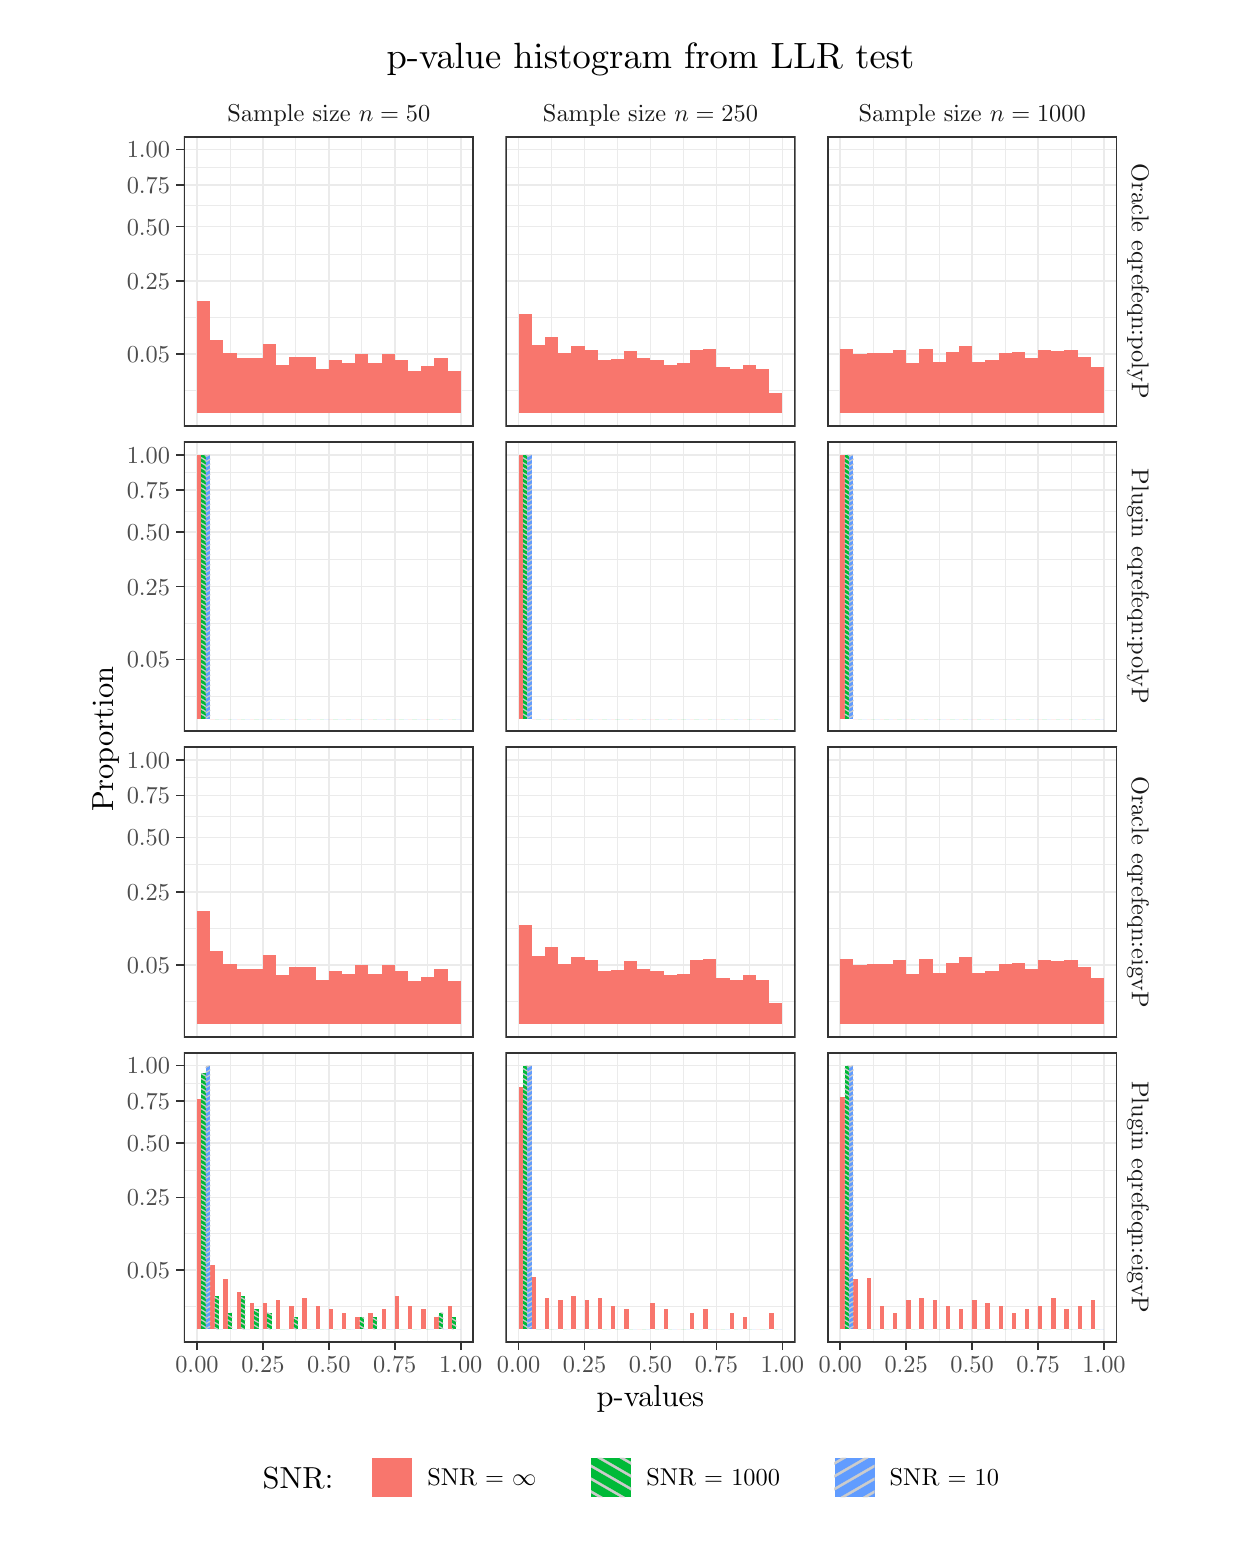
\begin{tikzpicture}[x=1pt,y=1pt]
\definecolor{fillColor}{RGB}{255,255,255}
\path[use as bounding box,fill=fillColor,fill opacity=0.00] (0,0) rectangle (433.62,542.02);
\begin{scope}
\path[clip] ( 17.85,  0.00) rectangle (415.77,542.02);
\definecolor{drawColor}{RGB}{255,255,255}
\definecolor{fillColor}{RGB}{255,255,255}

\path[draw=drawColor,line width= 0.6pt,line join=round,line cap=round,fill=fillColor] ( 17.85,  0.00) rectangle (415.77,542.02);
\end{scope}
\begin{scope}
\path[clip] ( 56.40,397.95) rectangle (161.25,502.80);
\definecolor{fillColor}{RGB}{255,255,255}

\path[fill=fillColor] ( 56.40,397.95) rectangle (161.25,502.80);
\definecolor{drawColor}{gray}{0.92}

\path[draw=drawColor,line width= 0.3pt,line join=round] ( 56.40,410.86) --
	(161.25,410.86);

\path[draw=drawColor,line width= 0.3pt,line join=round] ( 56.40,437.20) --
	(161.25,437.20);

\path[draw=drawColor,line width= 0.3pt,line join=round] ( 56.40,460.24) --
	(161.25,460.24);

\path[draw=drawColor,line width= 0.3pt,line join=round] ( 56.40,477.69) --
	(161.25,477.69);

\path[draw=drawColor,line width= 0.3pt,line join=round] ( 56.40,491.65) --
	(161.25,491.65);

\path[draw=drawColor,line width= 0.3pt,line join=round] ( 73.08,397.95) --
	( 73.08,502.80);

\path[draw=drawColor,line width= 0.3pt,line join=round] ( 96.91,397.95) --
	( 96.91,502.80);

\path[draw=drawColor,line width= 0.3pt,line join=round] (120.74,397.95) --
	(120.74,502.80);

\path[draw=drawColor,line width= 0.3pt,line join=round] (144.57,397.95) --
	(144.57,502.80);

\path[draw=drawColor,line width= 0.6pt,line join=round] ( 56.40,424.03) --
	(161.25,424.03);

\path[draw=drawColor,line width= 0.6pt,line join=round] ( 56.40,450.37) --
	(161.25,450.37);

\path[draw=drawColor,line width= 0.6pt,line join=round] ( 56.40,470.11) --
	(161.25,470.11);

\path[draw=drawColor,line width= 0.6pt,line join=round] ( 56.40,485.26) --
	(161.25,485.26);

\path[draw=drawColor,line width= 0.6pt,line join=round] ( 56.40,498.03) --
	(161.25,498.03);

\path[draw=drawColor,line width= 0.6pt,line join=round] ( 61.17,397.95) --
	( 61.17,502.80);

\path[draw=drawColor,line width= 0.6pt,line join=round] ( 85.00,397.95) --
	( 85.00,502.80);

\path[draw=drawColor,line width= 0.6pt,line join=round] (108.82,397.95) --
	(108.82,502.80);

\path[draw=drawColor,line width= 0.6pt,line join=round] (132.65,397.95) --
	(132.65,502.80);

\path[draw=drawColor,line width= 0.6pt,line join=round] (156.48,397.95) --
	(156.48,502.80);
\definecolor{fillColor}{RGB}{248,118,109}

\path[fill=fillColor] ( 61.17,402.72) rectangle ( 65.93,443.38);

\path[fill=fillColor] ( 65.93,402.72) rectangle ( 70.70,428.99);

\path[fill=fillColor] ( 70.70,402.72) rectangle ( 75.46,424.45);

\path[fill=fillColor] ( 75.46,402.72) rectangle ( 80.23,422.71);

\path[fill=fillColor] ( 80.23,402.72) rectangle ( 85.00,422.71);

\path[fill=fillColor] ( 85.00,402.72) rectangle ( 89.76,427.57);

\path[fill=fillColor] ( 89.76,402.72) rectangle ( 94.53,420.29);

\path[fill=fillColor] ( 94.53,402.72) rectangle ( 99.29,423.16);

\path[fill=fillColor] ( 99.29,402.72) rectangle (104.06,423.16);

\path[fill=fillColor] (104.06,402.72) rectangle (108.82,418.67);

\path[fill=fillColor] (108.82,402.72) rectangle (113.59,421.78);

\path[fill=fillColor] (113.59,402.72) rectangle (118.36,420.80);

\path[fill=fillColor] (118.36,402.72) rectangle (123.12,424.03);

\path[fill=fillColor] (123.12,402.72) rectangle (127.89,420.80);

\path[fill=fillColor] (127.89,402.72) rectangle (132.65,424.03);

\path[fill=fillColor] (132.65,402.72) rectangle (137.42,421.78);

\path[fill=fillColor] (137.42,402.72) rectangle (142.18,418.09);

\path[fill=fillColor] (142.18,402.72) rectangle (146.95,419.77);

\path[fill=fillColor] (146.95,402.72) rectangle (151.72,422.71);

\path[fill=fillColor] (151.72,402.72) rectangle (156.48,418.09);

\path[] ( 61.17,402.72) rectangle ( 65.93,443.38);

\path[] ( 65.93,402.72) rectangle ( 70.70,428.99);

\path[] ( 70.70,402.72) rectangle ( 75.46,424.45);

\path[] ( 75.46,402.72) rectangle ( 80.23,422.71);

\path[] ( 80.23,402.72) rectangle ( 85.00,422.71);

\path[] ( 85.00,402.72) rectangle ( 89.76,427.57);

\path[] ( 89.76,402.72) rectangle ( 94.53,420.29);

\path[] ( 94.53,402.72) rectangle ( 99.29,423.16);

\path[] ( 99.29,402.72) rectangle (104.06,423.16);

\path[] (104.06,402.72) rectangle (108.82,418.67);

\path[] (108.82,402.72) rectangle (113.59,421.78);

\path[] (113.59,402.72) rectangle (118.36,420.80);

\path[] (118.36,402.72) rectangle (123.12,424.03);

\path[] (123.12,402.72) rectangle (127.89,420.80);

\path[] (127.89,402.72) rectangle (132.65,424.03);

\path[] (132.65,402.72) rectangle (137.42,421.78);

\path[] (137.42,402.72) rectangle (142.18,418.09);

\path[] (142.18,402.72) rectangle (146.95,419.77);

\path[] (146.95,402.72) rectangle (151.72,422.71);

\path[] (151.72,402.72) rectangle (156.48,418.09);
\definecolor{drawColor}{gray}{0.20}

\path[draw=drawColor,line width= 1.1pt,line join=round,line cap=round] ( 56.40,397.95) rectangle (161.25,502.80);
\end{scope}
\begin{scope}
\path[clip] ( 56.40,287.60) rectangle (161.25,392.45);
\definecolor{fillColor}{RGB}{255,255,255}

\path[fill=fillColor] ( 56.40,287.60) rectangle (161.25,392.45);
\definecolor{drawColor}{gray}{0.92}

\path[draw=drawColor,line width= 0.3pt,line join=round] ( 56.40,300.51) --
	(161.25,300.51);

\path[draw=drawColor,line width= 0.3pt,line join=round] ( 56.40,326.86) --
	(161.25,326.86);

\path[draw=drawColor,line width= 0.3pt,line join=round] ( 56.40,349.90) --
	(161.25,349.90);

\path[draw=drawColor,line width= 0.3pt,line join=round] ( 56.40,367.34) --
	(161.25,367.34);

\path[draw=drawColor,line width= 0.3pt,line join=round] ( 56.40,381.30) --
	(161.25,381.30);

\path[draw=drawColor,line width= 0.3pt,line join=round] ( 73.08,287.60) --
	( 73.08,392.45);

\path[draw=drawColor,line width= 0.3pt,line join=round] ( 96.91,287.60) --
	( 96.91,392.45);

\path[draw=drawColor,line width= 0.3pt,line join=round] (120.74,287.60) --
	(120.74,392.45);

\path[draw=drawColor,line width= 0.3pt,line join=round] (144.57,287.60) --
	(144.57,392.45);

\path[draw=drawColor,line width= 0.6pt,line join=round] ( 56.40,313.68) --
	(161.25,313.68);

\path[draw=drawColor,line width= 0.6pt,line join=round] ( 56.40,340.03) --
	(161.25,340.03);

\path[draw=drawColor,line width= 0.6pt,line join=round] ( 56.40,359.77) --
	(161.25,359.77);

\path[draw=drawColor,line width= 0.6pt,line join=round] ( 56.40,374.91) --
	(161.25,374.91);

\path[draw=drawColor,line width= 0.6pt,line join=round] ( 56.40,387.68) --
	(161.25,387.68);

\path[draw=drawColor,line width= 0.6pt,line join=round] ( 61.17,287.60) --
	( 61.17,392.45);

\path[draw=drawColor,line width= 0.6pt,line join=round] ( 85.00,287.60) --
	( 85.00,392.45);

\path[draw=drawColor,line width= 0.6pt,line join=round] (108.82,287.60) --
	(108.82,392.45);

\path[draw=drawColor,line width= 0.6pt,line join=round] (132.65,287.60) --
	(132.65,392.45);

\path[draw=drawColor,line width= 0.6pt,line join=round] (156.48,287.60) --
	(156.48,392.45);
\definecolor{fillColor}{RGB}{248,118,109}

\path[fill=fillColor] ( 61.17,292.37) rectangle ( 62.76,387.68);

\path[fill=fillColor] ( 65.93,292.37) rectangle ( 67.52,292.37);

\path[fill=fillColor] ( 70.70,292.37) rectangle ( 72.29,292.37);

\path[fill=fillColor] ( 75.46,292.37) rectangle ( 77.05,292.37);

\path[fill=fillColor] ( 80.23,292.37) rectangle ( 81.82,292.37);

\path[fill=fillColor] ( 85.00,292.37) rectangle ( 86.58,292.37);

\path[fill=fillColor] ( 89.76,292.37) rectangle ( 91.35,292.37);

\path[fill=fillColor] ( 94.53,292.37) rectangle ( 96.12,292.37);

\path[fill=fillColor] ( 99.29,292.37) rectangle (100.88,292.37);

\path[fill=fillColor] (104.06,292.37) rectangle (105.65,292.37);

\path[fill=fillColor] (108.82,292.37) rectangle (110.41,292.37);

\path[fill=fillColor] (113.59,292.37) rectangle (115.18,292.37);

\path[fill=fillColor] (118.36,292.37) rectangle (119.94,292.37);

\path[fill=fillColor] (123.12,292.37) rectangle (124.71,292.37);

\path[fill=fillColor] (127.89,292.37) rectangle (129.48,292.37);

\path[fill=fillColor] (132.65,292.37) rectangle (134.24,292.37);

\path[fill=fillColor] (137.42,292.37) rectangle (139.01,292.37);

\path[fill=fillColor] (142.18,292.37) rectangle (143.77,292.37);

\path[fill=fillColor] (146.95,292.37) rectangle (148.54,292.37);

\path[fill=fillColor] (151.72,292.37) rectangle (153.30,292.37);
\definecolor{fillColor}{RGB}{0,186,56}

\path[fill=fillColor] ( 62.76,292.37) rectangle ( 64.34,387.68);

\path[fill=fillColor] ( 67.52,292.37) rectangle ( 69.11,292.37);

\path[fill=fillColor] ( 72.29,292.37) rectangle ( 73.88,292.37);

\path[fill=fillColor] ( 77.05,292.37) rectangle ( 78.64,292.37);

\path[fill=fillColor] ( 81.82,292.37) rectangle ( 83.41,292.37);

\path[fill=fillColor] ( 86.58,292.37) rectangle ( 88.17,292.37);

\path[fill=fillColor] ( 91.35,292.37) rectangle ( 92.94,292.37);

\path[fill=fillColor] ( 96.12,292.37) rectangle ( 97.70,292.37);

\path[fill=fillColor] (100.88,292.37) rectangle (102.47,292.37);

\path[fill=fillColor] (105.65,292.37) rectangle (107.24,292.37);

\path[fill=fillColor] (110.41,292.37) rectangle (112.00,292.37);

\path[fill=fillColor] (115.18,292.37) rectangle (116.77,292.37);

\path[fill=fillColor] (119.94,292.37) rectangle (121.53,292.37);

\path[fill=fillColor] (124.71,292.37) rectangle (126.30,292.37);

\path[fill=fillColor] (129.48,292.37) rectangle (131.06,292.37);

\path[fill=fillColor] (134.24,292.37) rectangle (135.83,292.37);

\path[fill=fillColor] (139.01,292.37) rectangle (140.60,292.37);

\path[fill=fillColor] (143.77,292.37) rectangle (145.36,292.37);

\path[fill=fillColor] (148.54,292.37) rectangle (150.13,292.37);

\path[fill=fillColor] (153.30,292.37) rectangle (154.89,292.37);
\definecolor{fillColor}{RGB}{97,156,255}

\path[fill=fillColor] ( 64.34,292.37) rectangle ( 65.93,387.68);

\path[fill=fillColor] ( 69.11,292.37) rectangle ( 70.70,292.37);

\path[fill=fillColor] ( 73.88,292.37) rectangle ( 75.46,292.37);

\path[fill=fillColor] ( 78.64,292.37) rectangle ( 80.23,292.37);

\path[fill=fillColor] ( 83.41,292.37) rectangle ( 85.00,292.37);

\path[fill=fillColor] ( 88.17,292.37) rectangle ( 89.76,292.37);

\path[fill=fillColor] ( 92.94,292.37) rectangle ( 94.53,292.37);

\path[fill=fillColor] ( 97.70,292.37) rectangle ( 99.29,292.37);

\path[fill=fillColor] (102.47,292.37) rectangle (104.06,292.37);

\path[fill=fillColor] (107.24,292.37) rectangle (108.82,292.37);

\path[fill=fillColor] (112.00,292.37) rectangle (113.59,292.37);

\path[fill=fillColor] (116.77,292.37) rectangle (118.36,292.37);

\path[fill=fillColor] (121.53,292.37) rectangle (123.12,292.37);

\path[fill=fillColor] (126.30,292.37) rectangle (127.89,292.37);

\path[fill=fillColor] (131.06,292.37) rectangle (132.65,292.37);

\path[fill=fillColor] (135.83,292.37) rectangle (137.42,292.37);

\path[fill=fillColor] (140.60,292.37) rectangle (142.18,292.37);

\path[fill=fillColor] (145.36,292.37) rectangle (146.95,292.37);

\path[fill=fillColor] (150.13,292.37) rectangle (151.72,292.37);

\path[fill=fillColor] (154.89,292.37) rectangle (156.48,292.37);
\definecolor{drawColor}{gray}{0.80}
\definecolor{fillColor}{gray}{0.80}

\path[draw=drawColor,line width= 0.1pt,line join=round,line cap=rect,fill=fillColor] ( 64.34,293.25) --
	( 64.34,292.89) --
	( 62.76,293.80) --
	( 62.76,294.17) --
	( 64.34,293.25) --
	cycle;

\path[draw=drawColor,line width= 0.1pt,line join=round,line cap=rect,fill=fillColor] ( 64.34,295.07) --
	( 64.34,294.70) --
	( 62.76,295.62) --
	( 62.76,295.98) --
	( 64.34,295.07) --
	cycle;

\path[draw=drawColor,line width= 0.1pt,line join=round,line cap=rect,fill=fillColor] ( 64.34,296.88) --
	( 64.34,296.52) --
	( 62.76,297.44) --
	( 62.76,297.80) --
	( 64.34,296.88) --
	cycle;

\path[draw=drawColor,line width= 0.1pt,line join=round,line cap=rect,fill=fillColor] ( 64.34,298.70) --
	( 64.34,298.33) --
	( 62.76,299.25) --
	( 62.76,299.62) --
	( 64.34,298.70) --
	cycle;

\path[draw=drawColor,line width= 0.1pt,line join=round,line cap=rect,fill=fillColor] ( 64.34,300.51) --
	( 64.34,300.15) --
	( 62.76,301.07) --
	( 62.76,301.43) --
	( 64.34,300.51) --
	cycle;

\path[draw=drawColor,line width= 0.1pt,line join=round,line cap=rect,fill=fillColor] ( 64.34,302.33) --
	( 64.34,301.97) --
	( 62.76,302.88) --
	( 62.76,303.25) --
	( 64.34,302.33) --
	cycle;

\path[draw=drawColor,line width= 0.1pt,line join=round,line cap=rect,fill=fillColor] ( 64.34,304.15) --
	( 64.34,303.78) --
	( 62.76,304.70) --
	( 62.76,305.06) --
	( 64.34,304.15) --
	cycle;

\path[draw=drawColor,line width= 0.1pt,line join=round,line cap=rect,fill=fillColor] ( 64.34,305.96) --
	( 64.34,305.60) --
	( 62.76,306.52) --
	( 62.76,306.88) --
	( 64.34,305.96) --
	cycle;

\path[draw=drawColor,line width= 0.1pt,line join=round,line cap=rect,fill=fillColor] ( 64.34,307.78) --
	( 64.34,307.41) --
	( 62.76,308.33) --
	( 62.76,308.70) --
	( 64.34,307.78) --
	cycle;

\path[draw=drawColor,line width= 0.1pt,line join=round,line cap=rect,fill=fillColor] ( 64.34,309.59) --
	( 64.34,309.23) --
	( 62.76,310.15) --
	( 62.76,310.51) --
	( 64.34,309.59) --
	cycle;

\path[draw=drawColor,line width= 0.1pt,line join=round,line cap=rect,fill=fillColor] ( 64.34,311.41) --
	( 64.34,311.05) --
	( 62.76,311.96) --
	( 62.76,312.33) --
	( 64.34,311.41) --
	cycle;

\path[draw=drawColor,line width= 0.1pt,line join=round,line cap=rect,fill=fillColor] ( 64.34,313.23) --
	( 64.34,312.86) --
	( 62.76,313.78) --
	( 62.76,314.14) --
	( 64.34,313.23) --
	cycle;

\path[draw=drawColor,line width= 0.1pt,line join=round,line cap=rect,fill=fillColor] ( 64.34,315.04) --
	( 64.34,314.68) --
	( 62.76,315.60) --
	( 62.76,315.96) --
	( 64.34,315.04) --
	cycle;

\path[draw=drawColor,line width= 0.1pt,line join=round,line cap=rect,fill=fillColor] ( 64.34,316.86) --
	( 64.34,316.49) --
	( 62.76,317.41) --
	( 62.76,317.78) --
	( 64.34,316.86) --
	cycle;

\path[draw=drawColor,line width= 0.1pt,line join=round,line cap=rect,fill=fillColor] ( 64.34,318.67) --
	( 64.34,318.31) --
	( 62.76,319.23) --
	( 62.76,319.59) --
	( 64.34,318.67) --
	cycle;

\path[draw=drawColor,line width= 0.1pt,line join=round,line cap=rect,fill=fillColor] ( 64.34,320.49) --
	( 64.34,320.13) --
	( 62.76,321.04) --
	( 62.76,321.41) --
	( 64.34,320.49) --
	cycle;

\path[draw=drawColor,line width= 0.1pt,line join=round,line cap=rect,fill=fillColor] ( 64.34,322.31) --
	( 64.34,321.94) --
	( 62.76,322.86) --
	( 62.76,323.22) --
	( 64.34,322.31) --
	cycle;

\path[draw=drawColor,line width= 0.1pt,line join=round,line cap=rect,fill=fillColor] ( 64.34,324.12) --
	( 64.34,323.76) --
	( 62.76,324.68) --
	( 62.76,325.04) --
	( 64.34,324.12) --
	cycle;

\path[draw=drawColor,line width= 0.1pt,line join=round,line cap=rect,fill=fillColor] ( 64.34,325.94) --
	( 64.34,325.57) --
	( 62.76,326.49) --
	( 62.76,326.85) --
	( 64.34,325.94) --
	cycle;

\path[draw=drawColor,line width= 0.1pt,line join=round,line cap=rect,fill=fillColor] ( 64.34,327.75) --
	( 64.34,327.39) --
	( 62.76,328.31) --
	( 62.76,328.67) --
	( 64.34,327.75) --
	cycle;

\path[draw=drawColor,line width= 0.1pt,line join=round,line cap=rect,fill=fillColor] ( 64.34,329.57) --
	( 64.34,329.21) --
	( 62.76,330.12) --
	( 62.76,330.49) --
	( 64.34,329.57) --
	cycle;

\path[draw=drawColor,line width= 0.1pt,line join=round,line cap=rect,fill=fillColor] ( 64.34,331.39) --
	( 64.34,331.02) --
	( 62.76,331.94) --
	( 62.76,332.30) --
	( 64.34,331.39) --
	cycle;

\path[draw=drawColor,line width= 0.1pt,line join=round,line cap=rect,fill=fillColor] ( 64.34,333.20) --
	( 64.34,332.84) --
	( 62.76,333.76) --
	( 62.76,334.12) --
	( 64.34,333.20) --
	cycle;

\path[draw=drawColor,line width= 0.1pt,line join=round,line cap=rect,fill=fillColor] ( 64.34,335.02) --
	( 64.34,334.65) --
	( 62.76,335.57) --
	( 62.76,335.93) --
	( 64.34,335.02) --
	cycle;

\path[draw=drawColor,line width= 0.1pt,line join=round,line cap=rect,fill=fillColor] ( 64.34,336.83) --
	( 64.34,336.47) --
	( 62.76,337.39) --
	( 62.76,337.75) --
	( 64.34,336.83) --
	cycle;

\path[draw=drawColor,line width= 0.1pt,line join=round,line cap=rect,fill=fillColor] ( 64.34,338.65) --
	( 64.34,338.29) --
	( 62.76,339.20) --
	( 62.76,339.57) --
	( 64.34,338.65) --
	cycle;

\path[draw=drawColor,line width= 0.1pt,line join=round,line cap=rect,fill=fillColor] ( 64.34,340.47) --
	( 64.34,340.10) --
	( 62.76,341.02) --
	( 62.76,341.38) --
	( 64.34,340.47) --
	cycle;

\path[draw=drawColor,line width= 0.1pt,line join=round,line cap=rect,fill=fillColor] ( 64.34,342.28) --
	( 64.34,341.92) --
	( 62.76,342.84) --
	( 62.76,343.20) --
	( 64.34,342.28) --
	cycle;

\path[draw=drawColor,line width= 0.1pt,line join=round,line cap=rect,fill=fillColor] ( 64.34,344.10) --
	( 64.34,343.73) --
	( 62.76,344.65) --
	( 62.76,345.01) --
	( 64.34,344.10) --
	cycle;

\path[draw=drawColor,line width= 0.1pt,line join=round,line cap=rect,fill=fillColor] ( 64.34,345.91) --
	( 64.34,345.55) --
	( 62.76,346.47) --
	( 62.76,346.83) --
	( 64.34,345.91) --
	cycle;

\path[draw=drawColor,line width= 0.1pt,line join=round,line cap=rect,fill=fillColor] ( 64.34,347.73) --
	( 64.34,347.37) --
	( 62.76,348.28) --
	( 62.76,348.65) --
	( 64.34,347.73) --
	cycle;

\path[draw=drawColor,line width= 0.1pt,line join=round,line cap=rect,fill=fillColor] ( 64.34,349.55) --
	( 64.34,349.18) --
	( 62.76,350.10) --
	( 62.76,350.46) --
	( 64.34,349.55) --
	cycle;

\path[draw=drawColor,line width= 0.1pt,line join=round,line cap=rect,fill=fillColor] ( 64.34,351.36) --
	( 64.34,351.00) --
	( 62.76,351.92) --
	( 62.76,352.28) --
	( 64.34,351.36) --
	cycle;

\path[draw=drawColor,line width= 0.1pt,line join=round,line cap=rect,fill=fillColor] ( 64.34,353.18) --
	( 64.34,352.81) --
	( 62.76,353.73) --
	( 62.76,354.09) --
	( 64.34,353.18) --
	cycle;

\path[draw=drawColor,line width= 0.1pt,line join=round,line cap=rect,fill=fillColor] ( 64.34,354.99) --
	( 64.34,354.63) --
	( 62.76,355.55) --
	( 62.76,355.91) --
	( 64.34,354.99) --
	cycle;

\path[draw=drawColor,line width= 0.1pt,line join=round,line cap=rect,fill=fillColor] ( 64.34,356.81) --
	( 64.34,356.45) --
	( 62.76,357.36) --
	( 62.76,357.73) --
	( 64.34,356.81) --
	cycle;

\path[draw=drawColor,line width= 0.1pt,line join=round,line cap=rect,fill=fillColor] ( 64.34,358.63) --
	( 64.34,358.26) --
	( 62.76,359.18) --
	( 62.76,359.54) --
	( 64.34,358.63) --
	cycle;

\path[draw=drawColor,line width= 0.1pt,line join=round,line cap=rect,fill=fillColor] ( 64.34,360.44) --
	( 64.34,360.08) --
	( 62.76,361.00) --
	( 62.76,361.36) --
	( 64.34,360.44) --
	cycle;

\path[draw=drawColor,line width= 0.1pt,line join=round,line cap=rect,fill=fillColor] ( 64.34,362.26) --
	( 64.34,361.89) --
	( 62.76,362.81) --
	( 62.76,363.17) --
	( 64.34,362.26) --
	cycle;

\path[draw=drawColor,line width= 0.1pt,line join=round,line cap=rect,fill=fillColor] ( 64.34,364.07) --
	( 64.34,363.71) --
	( 62.76,364.63) --
	( 62.76,364.99) --
	( 64.34,364.07) --
	cycle;

\path[draw=drawColor,line width= 0.1pt,line join=round,line cap=rect,fill=fillColor] ( 64.34,365.89) --
	( 64.34,365.53) --
	( 62.76,366.44) --
	( 62.76,366.81) --
	( 64.34,365.89) --
	cycle;

\path[draw=drawColor,line width= 0.1pt,line join=round,line cap=rect,fill=fillColor] ( 64.34,367.71) --
	( 64.34,367.34) --
	( 62.76,368.26) --
	( 62.76,368.62) --
	( 64.34,367.71) --
	cycle;

\path[draw=drawColor,line width= 0.1pt,line join=round,line cap=rect,fill=fillColor] ( 64.34,369.52) --
	( 64.34,369.16) --
	( 62.76,370.08) --
	( 62.76,370.44) --
	( 64.34,369.52) --
	cycle;

\path[draw=drawColor,line width= 0.1pt,line join=round,line cap=rect,fill=fillColor] ( 64.34,371.34) --
	( 64.34,370.97) --
	( 62.76,371.89) --
	( 62.76,372.25) --
	( 64.34,371.34) --
	cycle;

\path[draw=drawColor,line width= 0.1pt,line join=round,line cap=rect,fill=fillColor] ( 64.34,373.15) --
	( 64.34,372.79) --
	( 62.76,373.71) --
	( 62.76,374.07) --
	( 64.34,373.15) --
	cycle;

\path[draw=drawColor,line width= 0.1pt,line join=round,line cap=rect,fill=fillColor] ( 64.34,374.97) --
	( 64.34,374.61) --
	( 62.76,375.52) --
	( 62.76,375.89) --
	( 64.34,374.97) --
	cycle;

\path[draw=drawColor,line width= 0.1pt,line join=round,line cap=rect,fill=fillColor] ( 64.34,376.79) --
	( 64.34,376.42) --
	( 62.76,377.34) --
	( 62.76,377.70) --
	( 64.34,376.79) --
	cycle;

\path[draw=drawColor,line width= 0.1pt,line join=round,line cap=rect,fill=fillColor] ( 64.34,378.60) --
	( 64.34,378.24) --
	( 62.76,379.16) --
	( 62.76,379.52) --
	( 64.34,378.60) --
	cycle;

\path[draw=drawColor,line width= 0.1pt,line join=round,line cap=rect,fill=fillColor] ( 64.34,380.42) --
	( 64.34,380.05) --
	( 62.76,380.97) --
	( 62.76,381.33) --
	( 64.34,380.42) --
	cycle;

\path[draw=drawColor,line width= 0.1pt,line join=round,line cap=rect,fill=fillColor] ( 64.34,382.23) --
	( 64.34,381.87) --
	( 62.76,382.79) --
	( 62.76,383.15) --
	( 64.34,382.23) --
	cycle;

\path[draw=drawColor,line width= 0.1pt,line join=round,line cap=rect,fill=fillColor] ( 64.34,384.05) --
	( 64.34,383.69) --
	( 62.76,384.60) --
	( 62.76,384.97) --
	( 64.34,384.05) --
	cycle;

\path[draw=drawColor,line width= 0.1pt,line join=round,line cap=rect,fill=fillColor] ( 64.34,385.87) --
	( 64.34,385.50) --
	( 62.76,386.42) --
	( 62.76,386.78) --
	( 64.34,385.87) --
	cycle;

\path[draw=drawColor,line width= 0.1pt,line join=round,line cap=rect,fill=fillColor] ( 64.34,387.68) --
	( 64.34,387.32) --
	( 63.71,387.68) --
	( 64.34,387.68) --
	( 64.34,387.68) --
	cycle;

\path[draw=drawColor,line width= 0.1pt,line join=round,line cap=rect,fill=fillColor] ( 65.93,293.65) --
	( 65.93,293.29) --
	( 64.34,292.37) --
	( 64.34,292.74) --
	( 65.93,293.65) --
	cycle;

\path[draw=drawColor,line width= 0.1pt,line join=round,line cap=rect,fill=fillColor] ( 65.93,295.47) --
	( 65.93,295.11) --
	( 64.34,294.19) --
	( 64.34,294.55) --
	( 65.93,295.47) --
	cycle;

\path[draw=drawColor,line width= 0.1pt,line join=round,line cap=rect,fill=fillColor] ( 65.93,297.29) --
	( 65.93,296.92) --
	( 64.34,296.01) --
	( 64.34,296.37) --
	( 65.93,297.29) --
	cycle;

\path[draw=drawColor,line width= 0.1pt,line join=round,line cap=rect,fill=fillColor] ( 65.93,299.10) --
	( 65.93,298.74) --
	( 64.34,297.82) --
	( 64.34,298.18) --
	( 65.93,299.10) --
	cycle;

\path[draw=drawColor,line width= 0.1pt,line join=round,line cap=rect,fill=fillColor] ( 65.93,300.92) --
	( 65.93,300.55) --
	( 64.34,299.64) --
	( 64.34,300.00) --
	( 65.93,300.92) --
	cycle;

\path[draw=drawColor,line width= 0.1pt,line join=round,line cap=rect,fill=fillColor] ( 65.93,302.73) --
	( 65.93,302.37) --
	( 64.34,301.45) --
	( 64.34,301.82) --
	( 65.93,302.73) --
	cycle;

\path[draw=drawColor,line width= 0.1pt,line join=round,line cap=rect,fill=fillColor] ( 65.93,304.55) --
	( 65.93,304.19) --
	( 64.34,303.27) --
	( 64.34,303.63) --
	( 65.93,304.55) --
	cycle;

\path[draw=drawColor,line width= 0.1pt,line join=round,line cap=rect,fill=fillColor] ( 65.93,306.37) --
	( 65.93,306.00) --
	( 64.34,305.09) --
	( 64.34,305.45) --
	( 65.93,306.37) --
	cycle;

\path[draw=drawColor,line width= 0.1pt,line join=round,line cap=rect,fill=fillColor] ( 65.93,308.18) --
	( 65.93,307.82) --
	( 64.34,306.90) --
	( 64.34,307.26) --
	( 65.93,308.18) --
	cycle;

\path[draw=drawColor,line width= 0.1pt,line join=round,line cap=rect,fill=fillColor] ( 65.93,310.00) --
	( 65.93,309.63) --
	( 64.34,308.72) --
	( 64.34,309.08) --
	( 65.93,310.00) --
	cycle;

\path[draw=drawColor,line width= 0.1pt,line join=round,line cap=rect,fill=fillColor] ( 65.93,311.81) --
	( 65.93,311.45) --
	( 64.34,310.53) --
	( 64.34,310.90) --
	( 65.93,311.81) --
	cycle;

\path[draw=drawColor,line width= 0.1pt,line join=round,line cap=rect,fill=fillColor] ( 65.93,313.63) --
	( 65.93,313.27) --
	( 64.34,312.35) --
	( 64.34,312.71) --
	( 65.93,313.63) --
	cycle;

\path[draw=drawColor,line width= 0.1pt,line join=round,line cap=rect,fill=fillColor] ( 65.93,315.45) --
	( 65.93,315.08) --
	( 64.34,314.17) --
	( 64.34,314.53) --
	( 65.93,315.45) --
	cycle;

\path[draw=drawColor,line width= 0.1pt,line join=round,line cap=rect,fill=fillColor] ( 65.93,317.26) --
	( 65.93,316.90) --
	( 64.34,315.98) --
	( 64.34,316.34) --
	( 65.93,317.26) --
	cycle;

\path[draw=drawColor,line width= 0.1pt,line join=round,line cap=rect,fill=fillColor] ( 65.93,319.08) --
	( 65.93,318.71) --
	( 64.34,317.80) --
	( 64.34,318.16) --
	( 65.93,319.08) --
	cycle;

\path[draw=drawColor,line width= 0.1pt,line join=round,line cap=rect,fill=fillColor] ( 65.93,320.89) --
	( 65.93,320.53) --
	( 64.34,319.61) --
	( 64.34,319.98) --
	( 65.93,320.89) --
	cycle;

\path[draw=drawColor,line width= 0.1pt,line join=round,line cap=rect,fill=fillColor] ( 65.93,322.71) --
	( 65.93,322.35) --
	( 64.34,321.43) --
	( 64.34,321.79) --
	( 65.93,322.71) --
	cycle;

\path[draw=drawColor,line width= 0.1pt,line join=round,line cap=rect,fill=fillColor] ( 65.93,324.53) --
	( 65.93,324.16) --
	( 64.34,323.24) --
	( 64.34,323.61) --
	( 65.93,324.53) --
	cycle;

\path[draw=drawColor,line width= 0.1pt,line join=round,line cap=rect,fill=fillColor] ( 65.93,326.34) --
	( 65.93,325.98) --
	( 64.34,325.06) --
	( 64.34,325.42) --
	( 65.93,326.34) --
	cycle;

\path[draw=drawColor,line width= 0.1pt,line join=round,line cap=rect,fill=fillColor] ( 65.93,328.16) --
	( 65.93,327.79) --
	( 64.34,326.88) --
	( 64.34,327.24) --
	( 65.93,328.16) --
	cycle;

\path[draw=drawColor,line width= 0.1pt,line join=round,line cap=rect,fill=fillColor] ( 65.93,329.97) --
	( 65.93,329.61) --
	( 64.34,328.69) --
	( 64.34,329.06) --
	( 65.93,329.97) --
	cycle;

\path[draw=drawColor,line width= 0.1pt,line join=round,line cap=rect,fill=fillColor] ( 65.93,331.79) --
	( 65.93,331.43) --
	( 64.34,330.51) --
	( 64.34,330.87) --
	( 65.93,331.79) --
	cycle;

\path[draw=drawColor,line width= 0.1pt,line join=round,line cap=rect,fill=fillColor] ( 65.93,333.61) --
	( 65.93,333.24) --
	( 64.34,332.32) --
	( 64.34,332.69) --
	( 65.93,333.61) --
	cycle;

\path[draw=drawColor,line width= 0.1pt,line join=round,line cap=rect,fill=fillColor] ( 65.93,335.42) --
	( 65.93,335.06) --
	( 64.34,334.14) --
	( 64.34,334.50) --
	( 65.93,335.42) --
	cycle;

\path[draw=drawColor,line width= 0.1pt,line join=round,line cap=rect,fill=fillColor] ( 65.93,337.24) --
	( 65.93,336.87) --
	( 64.34,335.96) --
	( 64.34,336.32) --
	( 65.93,337.24) --
	cycle;

\path[draw=drawColor,line width= 0.1pt,line join=round,line cap=rect,fill=fillColor] ( 65.93,339.05) --
	( 65.93,338.69) --
	( 64.34,337.77) --
	( 64.34,338.14) --
	( 65.93,339.05) --
	cycle;

\path[draw=drawColor,line width= 0.1pt,line join=round,line cap=rect,fill=fillColor] ( 65.93,340.87) --
	( 65.93,340.51) --
	( 64.34,339.59) --
	( 64.34,339.95) --
	( 65.93,340.87) --
	cycle;

\path[draw=drawColor,line width= 0.1pt,line join=round,line cap=rect,fill=fillColor] ( 65.93,342.69) --
	( 65.93,342.32) --
	( 64.34,341.40) --
	( 64.34,341.77) --
	( 65.93,342.69) --
	cycle;

\path[draw=drawColor,line width= 0.1pt,line join=round,line cap=rect,fill=fillColor] ( 65.93,344.50) --
	( 65.93,344.14) --
	( 64.34,343.22) --
	( 64.34,343.58) --
	( 65.93,344.50) --
	cycle;

\path[draw=drawColor,line width= 0.1pt,line join=round,line cap=rect,fill=fillColor] ( 65.93,346.32) --
	( 65.93,345.95) --
	( 64.34,345.04) --
	( 64.34,345.40) --
	( 65.93,346.32) --
	cycle;

\path[draw=drawColor,line width= 0.1pt,line join=round,line cap=rect,fill=fillColor] ( 65.93,348.13) --
	( 65.93,347.77) --
	( 64.34,346.85) --
	( 64.34,347.22) --
	( 65.93,348.13) --
	cycle;

\path[draw=drawColor,line width= 0.1pt,line join=round,line cap=rect,fill=fillColor] ( 65.93,349.95) --
	( 65.93,349.59) --
	( 64.34,348.67) --
	( 64.34,349.03) --
	( 65.93,349.95) --
	cycle;

\path[draw=drawColor,line width= 0.1pt,line join=round,line cap=rect,fill=fillColor] ( 65.93,351.77) --
	( 65.93,351.40) --
	( 64.34,350.48) --
	( 64.34,350.85) --
	( 65.93,351.77) --
	cycle;

\path[draw=drawColor,line width= 0.1pt,line join=round,line cap=rect,fill=fillColor] ( 65.93,353.58) --
	( 65.93,353.22) --
	( 64.34,352.30) --
	( 64.34,352.66) --
	( 65.93,353.58) --
	cycle;

\path[draw=drawColor,line width= 0.1pt,line join=round,line cap=rect,fill=fillColor] ( 65.93,355.40) --
	( 65.93,355.03) --
	( 64.34,354.12) --
	( 64.34,354.48) --
	( 65.93,355.40) --
	cycle;

\path[draw=drawColor,line width= 0.1pt,line join=round,line cap=rect,fill=fillColor] ( 65.93,357.21) --
	( 65.93,356.85) --
	( 64.34,355.93) --
	( 64.34,356.30) --
	( 65.93,357.21) --
	cycle;

\path[draw=drawColor,line width= 0.1pt,line join=round,line cap=rect,fill=fillColor] ( 65.93,359.03) --
	( 65.93,358.67) --
	( 64.34,357.75) --
	( 64.34,358.11) --
	( 65.93,359.03) --
	cycle;

\path[draw=drawColor,line width= 0.1pt,line join=round,line cap=rect,fill=fillColor] ( 65.93,360.85) --
	( 65.93,360.48) --
	( 64.34,359.56) --
	( 64.34,359.93) --
	( 65.93,360.85) --
	cycle;

\path[draw=drawColor,line width= 0.1pt,line join=round,line cap=rect,fill=fillColor] ( 65.93,362.66) --
	( 65.93,362.30) --
	( 64.34,361.38) --
	( 64.34,361.74) --
	( 65.93,362.66) --
	cycle;

\path[draw=drawColor,line width= 0.1pt,line join=round,line cap=rect,fill=fillColor] ( 65.93,364.48) --
	( 65.93,364.11) --
	( 64.34,363.20) --
	( 64.34,363.56) --
	( 65.93,364.48) --
	cycle;

\path[draw=drawColor,line width= 0.1pt,line join=round,line cap=rect,fill=fillColor] ( 65.93,366.29) --
	( 65.93,365.93) --
	( 64.34,365.01) --
	( 64.34,365.38) --
	( 65.93,366.29) --
	cycle;

\path[draw=drawColor,line width= 0.1pt,line join=round,line cap=rect,fill=fillColor] ( 65.93,368.11) --
	( 65.93,367.75) --
	( 64.34,366.83) --
	( 64.34,367.19) --
	( 65.93,368.11) --
	cycle;

\path[draw=drawColor,line width= 0.1pt,line join=round,line cap=rect,fill=fillColor] ( 65.93,369.93) --
	( 65.93,369.56) --
	( 64.34,368.64) --
	( 64.34,369.01) --
	( 65.93,369.93) --
	cycle;

\path[draw=drawColor,line width= 0.1pt,line join=round,line cap=rect,fill=fillColor] ( 65.93,371.74) --
	( 65.93,371.38) --
	( 64.34,370.46) --
	( 64.34,370.82) --
	( 65.93,371.74) --
	cycle;

\path[draw=drawColor,line width= 0.1pt,line join=round,line cap=rect,fill=fillColor] ( 65.93,373.56) --
	( 65.93,373.19) --
	( 64.34,372.28) --
	( 64.34,372.64) --
	( 65.93,373.56) --
	cycle;

\path[draw=drawColor,line width= 0.1pt,line join=round,line cap=rect,fill=fillColor] ( 65.93,375.37) --
	( 65.93,375.01) --
	( 64.34,374.09) --
	( 64.34,374.46) --
	( 65.93,375.37) --
	cycle;

\path[draw=drawColor,line width= 0.1pt,line join=round,line cap=rect,fill=fillColor] ( 65.93,377.19) --
	( 65.93,376.83) --
	( 64.34,375.91) --
	( 64.34,376.27) --
	( 65.93,377.19) --
	cycle;

\path[draw=drawColor,line width= 0.1pt,line join=round,line cap=rect,fill=fillColor] ( 65.93,379.00) --
	( 65.93,378.64) --
	( 64.34,377.72) --
	( 64.34,378.09) --
	( 65.93,379.00) --
	cycle;

\path[draw=drawColor,line width= 0.1pt,line join=round,line cap=rect,fill=fillColor] ( 65.93,380.82) --
	( 65.93,380.46) --
	( 64.34,379.54) --
	( 64.34,379.90) --
	( 65.93,380.82) --
	cycle;

\path[draw=drawColor,line width= 0.1pt,line join=round,line cap=rect,fill=fillColor] ( 65.93,382.64) --
	( 65.93,382.27) --
	( 64.34,381.36) --
	( 64.34,381.72) --
	( 65.93,382.64) --
	cycle;

\path[draw=drawColor,line width= 0.1pt,line join=round,line cap=rect,fill=fillColor] ( 65.93,384.45) --
	( 65.93,384.09) --
	( 64.34,383.17) --
	( 64.34,383.54) --
	( 65.93,384.45) --
	cycle;

\path[draw=drawColor,line width= 0.1pt,line join=round,line cap=rect,fill=fillColor] ( 65.93,386.27) --
	( 65.93,385.91) --
	( 64.34,384.99) --
	( 64.34,385.35) --
	( 65.93,386.27) --
	cycle;

\path[draw=drawColor,line width= 0.1pt,line join=round,line cap=rect,fill=fillColor] ( 65.24,387.68) --
	( 65.87,387.68) --
	( 64.34,386.80) --
	( 64.34,387.17) --
	( 65.24,387.68) --
	cycle;

\path[] ( 61.17,292.37) rectangle ( 62.76,387.68);

\path[] ( 65.93,292.37) rectangle ( 67.52,292.37);

\path[] ( 70.70,292.37) rectangle ( 72.29,292.37);

\path[] ( 75.46,292.37) rectangle ( 77.05,292.37);

\path[] ( 80.23,292.37) rectangle ( 81.82,292.37);

\path[] ( 85.00,292.37) rectangle ( 86.58,292.37);

\path[] ( 89.76,292.37) rectangle ( 91.35,292.37);

\path[] ( 94.53,292.37) rectangle ( 96.12,292.37);

\path[] ( 99.29,292.37) rectangle (100.88,292.37);

\path[] (104.06,292.37) rectangle (105.65,292.37);

\path[] (108.82,292.37) rectangle (110.41,292.37);

\path[] (113.59,292.37) rectangle (115.18,292.37);

\path[] (118.36,292.37) rectangle (119.94,292.37);

\path[] (123.12,292.37) rectangle (124.71,292.37);

\path[] (127.89,292.37) rectangle (129.48,292.37);

\path[] (132.65,292.37) rectangle (134.24,292.37);

\path[] (137.42,292.37) rectangle (139.01,292.37);

\path[] (142.18,292.37) rectangle (143.77,292.37);

\path[] (146.95,292.37) rectangle (148.54,292.37);

\path[] (151.72,292.37) rectangle (153.30,292.37);

\path[] ( 62.76,292.37) rectangle ( 64.34,387.68);

\path[] ( 67.52,292.37) rectangle ( 69.11,292.37);

\path[] ( 72.29,292.37) rectangle ( 73.88,292.37);

\path[] ( 77.05,292.37) rectangle ( 78.64,292.37);

\path[] ( 81.82,292.37) rectangle ( 83.41,292.37);

\path[] ( 86.58,292.37) rectangle ( 88.17,292.37);

\path[] ( 91.35,292.37) rectangle ( 92.94,292.37);

\path[] ( 96.12,292.37) rectangle ( 97.70,292.37);

\path[] (100.88,292.37) rectangle (102.47,292.37);

\path[] (105.65,292.37) rectangle (107.24,292.37);

\path[] (110.41,292.37) rectangle (112.00,292.37);

\path[] (115.18,292.37) rectangle (116.77,292.37);

\path[] (119.94,292.37) rectangle (121.53,292.37);

\path[] (124.71,292.37) rectangle (126.30,292.37);

\path[] (129.48,292.37) rectangle (131.06,292.37);

\path[] (134.24,292.37) rectangle (135.83,292.37);

\path[] (139.01,292.37) rectangle (140.60,292.37);

\path[] (143.77,292.37) rectangle (145.36,292.37);

\path[] (148.54,292.37) rectangle (150.13,292.37);

\path[] (153.30,292.37) rectangle (154.89,292.37);

\path[] ( 64.34,292.37) rectangle ( 65.93,387.68);

\path[] ( 69.11,292.37) rectangle ( 70.70,292.37);

\path[] ( 73.88,292.37) rectangle ( 75.46,292.37);

\path[] ( 78.64,292.37) rectangle ( 80.23,292.37);

\path[] ( 83.41,292.37) rectangle ( 85.00,292.37);

\path[] ( 88.17,292.37) rectangle ( 89.76,292.37);

\path[] ( 92.94,292.37) rectangle ( 94.53,292.37);

\path[] ( 97.70,292.37) rectangle ( 99.29,292.37);

\path[] (102.47,292.37) rectangle (104.06,292.37);

\path[] (107.24,292.37) rectangle (108.82,292.37);

\path[] (112.00,292.37) rectangle (113.59,292.37);

\path[] (116.77,292.37) rectangle (118.36,292.37);

\path[] (121.53,292.37) rectangle (123.12,292.37);

\path[] (126.30,292.37) rectangle (127.89,292.37);

\path[] (131.06,292.37) rectangle (132.65,292.37);

\path[] (135.83,292.37) rectangle (137.42,292.37);

\path[] (140.60,292.37) rectangle (142.18,292.37);

\path[] (145.36,292.37) rectangle (146.95,292.37);

\path[] (150.13,292.37) rectangle (151.72,292.37);

\path[] (154.89,292.37) rectangle (156.48,292.37);
\definecolor{drawColor}{gray}{0.20}

\path[draw=drawColor,line width= 1.1pt,line join=round,line cap=round] ( 56.40,287.60) rectangle (161.25,392.45);
\end{scope}
\begin{scope}
\path[clip] ( 56.40,177.26) rectangle (161.25,282.10);
\definecolor{fillColor}{RGB}{255,255,255}

\path[fill=fillColor] ( 56.40,177.26) rectangle (161.25,282.10);
\definecolor{drawColor}{gray}{0.92}

\path[draw=drawColor,line width= 0.3pt,line join=round] ( 56.40,190.16) --
	(161.25,190.16);

\path[draw=drawColor,line width= 0.3pt,line join=round] ( 56.40,216.51) --
	(161.25,216.51);

\path[draw=drawColor,line width= 0.3pt,line join=round] ( 56.40,239.55) --
	(161.25,239.55);

\path[draw=drawColor,line width= 0.3pt,line join=round] ( 56.40,257.00) --
	(161.25,257.00);

\path[draw=drawColor,line width= 0.3pt,line join=round] ( 56.40,270.95) --
	(161.25,270.95);

\path[draw=drawColor,line width= 0.3pt,line join=round] ( 73.08,177.26) --
	( 73.08,282.10);

\path[draw=drawColor,line width= 0.3pt,line join=round] ( 96.91,177.26) --
	( 96.91,282.10);

\path[draw=drawColor,line width= 0.3pt,line join=round] (120.74,177.26) --
	(120.74,282.10);

\path[draw=drawColor,line width= 0.3pt,line join=round] (144.57,177.26) --
	(144.57,282.10);

\path[draw=drawColor,line width= 0.6pt,line join=round] ( 56.40,203.34) --
	(161.25,203.34);

\path[draw=drawColor,line width= 0.6pt,line join=round] ( 56.40,229.68) --
	(161.25,229.68);

\path[draw=drawColor,line width= 0.6pt,line join=round] ( 56.40,249.42) --
	(161.25,249.42);

\path[draw=drawColor,line width= 0.6pt,line join=round] ( 56.40,264.57) --
	(161.25,264.57);

\path[draw=drawColor,line width= 0.6pt,line join=round] ( 56.40,277.34) --
	(161.25,277.34);

\path[draw=drawColor,line width= 0.6pt,line join=round] ( 61.17,177.26) --
	( 61.17,282.10);

\path[draw=drawColor,line width= 0.6pt,line join=round] ( 85.00,177.26) --
	( 85.00,282.10);

\path[draw=drawColor,line width= 0.6pt,line join=round] (108.82,177.26) --
	(108.82,282.10);

\path[draw=drawColor,line width= 0.6pt,line join=round] (132.65,177.26) --
	(132.65,282.10);

\path[draw=drawColor,line width= 0.6pt,line join=round] (156.48,177.26) --
	(156.48,282.10);
\definecolor{fillColor}{RGB}{248,118,109}

\path[fill=fillColor] ( 61.17,182.02) rectangle ( 65.93,222.69);

\path[fill=fillColor] ( 65.93,182.02) rectangle ( 70.70,208.30);

\path[fill=fillColor] ( 70.70,182.02) rectangle ( 75.46,203.76);

\path[fill=fillColor] ( 75.46,182.02) rectangle ( 80.23,202.02);

\path[fill=fillColor] ( 80.23,182.02) rectangle ( 85.00,202.02);

\path[fill=fillColor] ( 85.00,182.02) rectangle ( 89.76,206.88);

\path[fill=fillColor] ( 89.76,182.02) rectangle ( 94.53,199.60);

\path[fill=fillColor] ( 94.53,182.02) rectangle ( 99.29,202.47);

\path[fill=fillColor] ( 99.29,182.02) rectangle (104.06,202.47);

\path[fill=fillColor] (104.06,182.02) rectangle (108.82,197.97);

\path[fill=fillColor] (108.82,182.02) rectangle (113.59,201.09);

\path[fill=fillColor] (113.59,182.02) rectangle (118.36,200.11);

\path[fill=fillColor] (118.36,182.02) rectangle (123.12,203.34);

\path[fill=fillColor] (123.12,182.02) rectangle (127.89,200.11);

\path[fill=fillColor] (127.89,182.02) rectangle (132.65,203.34);

\path[fill=fillColor] (132.65,182.02) rectangle (137.42,201.09);

\path[fill=fillColor] (137.42,182.02) rectangle (142.18,197.39);

\path[fill=fillColor] (142.18,182.02) rectangle (146.95,199.07);

\path[fill=fillColor] (146.95,182.02) rectangle (151.72,202.02);

\path[fill=fillColor] (151.72,182.02) rectangle (156.48,197.39);

\path[] ( 61.17,182.02) rectangle ( 65.93,222.69);

\path[] ( 65.93,182.02) rectangle ( 70.70,208.30);

\path[] ( 70.70,182.02) rectangle ( 75.46,203.76);

\path[] ( 75.46,182.02) rectangle ( 80.23,202.02);

\path[] ( 80.23,182.02) rectangle ( 85.00,202.02);

\path[] ( 85.00,182.02) rectangle ( 89.76,206.88);

\path[] ( 89.76,182.02) rectangle ( 94.53,199.60);

\path[] ( 94.53,182.02) rectangle ( 99.29,202.47);

\path[] ( 99.29,182.02) rectangle (104.06,202.47);

\path[] (104.06,182.02) rectangle (108.82,197.97);

\path[] (108.82,182.02) rectangle (113.59,201.09);

\path[] (113.59,182.02) rectangle (118.36,200.11);

\path[] (118.36,182.02) rectangle (123.12,203.34);

\path[] (123.12,182.02) rectangle (127.89,200.11);

\path[] (127.89,182.02) rectangle (132.65,203.34);

\path[] (132.65,182.02) rectangle (137.42,201.09);

\path[] (137.42,182.02) rectangle (142.18,197.39);

\path[] (142.18,182.02) rectangle (146.95,199.07);

\path[] (146.95,182.02) rectangle (151.72,202.02);

\path[] (151.72,182.02) rectangle (156.48,197.39);
\definecolor{drawColor}{gray}{0.20}

\path[draw=drawColor,line width= 1.1pt,line join=round,line cap=round] ( 56.40,177.26) rectangle (161.25,282.10);
\end{scope}
\begin{scope}
\path[clip] ( 56.40, 66.91) rectangle (161.25,171.76);
\definecolor{fillColor}{RGB}{255,255,255}

\path[fill=fillColor] ( 56.40, 66.91) rectangle (161.25,171.76);
\definecolor{drawColor}{gray}{0.92}

\path[draw=drawColor,line width= 0.3pt,line join=round] ( 56.40, 79.82) --
	(161.25, 79.82);

\path[draw=drawColor,line width= 0.3pt,line join=round] ( 56.40,106.16) --
	(161.25,106.16);

\path[draw=drawColor,line width= 0.3pt,line join=round] ( 56.40,129.21) --
	(161.25,129.21);

\path[draw=drawColor,line width= 0.3pt,line join=round] ( 56.40,146.65) --
	(161.25,146.65);

\path[draw=drawColor,line width= 0.3pt,line join=round] ( 56.40,160.61) --
	(161.25,160.61);

\path[draw=drawColor,line width= 0.3pt,line join=round] ( 73.08, 66.91) --
	( 73.08,171.76);

\path[draw=drawColor,line width= 0.3pt,line join=round] ( 96.91, 66.91) --
	( 96.91,171.76);

\path[draw=drawColor,line width= 0.3pt,line join=round] (120.74, 66.91) --
	(120.74,171.76);

\path[draw=drawColor,line width= 0.3pt,line join=round] (144.57, 66.91) --
	(144.57,171.76);

\path[draw=drawColor,line width= 0.6pt,line join=round] ( 56.40, 92.99) --
	(161.25, 92.99);

\path[draw=drawColor,line width= 0.6pt,line join=round] ( 56.40,119.34) --
	(161.25,119.34);

\path[draw=drawColor,line width= 0.6pt,line join=round] ( 56.40,139.08) --
	(161.25,139.08);

\path[draw=drawColor,line width= 0.6pt,line join=round] ( 56.40,154.22) --
	(161.25,154.22);

\path[draw=drawColor,line width= 0.6pt,line join=round] ( 56.40,166.99) --
	(161.25,166.99);

\path[draw=drawColor,line width= 0.6pt,line join=round] ( 61.17, 66.91) --
	( 61.17,171.76);

\path[draw=drawColor,line width= 0.6pt,line join=round] ( 85.00, 66.91) --
	( 85.00,171.76);

\path[draw=drawColor,line width= 0.6pt,line join=round] (108.82, 66.91) --
	(108.82,171.76);

\path[draw=drawColor,line width= 0.6pt,line join=round] (132.65, 66.91) --
	(132.65,171.76);

\path[draw=drawColor,line width= 0.6pt,line join=round] (156.48, 66.91) --
	(156.48,171.76);
\definecolor{fillColor}{RGB}{248,118,109}

\path[fill=fillColor] ( 61.17, 71.68) rectangle ( 62.76,154.77);

\path[fill=fillColor] ( 65.93, 71.68) rectangle ( 67.52, 95.03);

\path[fill=fillColor] ( 70.70, 71.68) rectangle ( 72.29, 89.76);

\path[fill=fillColor] ( 75.46, 71.68) rectangle ( 77.05, 85.16);

\path[fill=fillColor] ( 80.23, 71.68) rectangle ( 81.82, 81.21);

\path[fill=fillColor] ( 85.00, 71.68) rectangle ( 86.58, 81.21);

\path[fill=fillColor] ( 89.76, 71.68) rectangle ( 91.35, 82.12);

\path[fill=fillColor] ( 94.53, 71.68) rectangle ( 96.12, 80.20);

\path[fill=fillColor] ( 99.29, 71.68) rectangle (100.88, 82.96);

\path[fill=fillColor] (104.06, 71.68) rectangle (105.65, 80.20);

\path[fill=fillColor] (108.82, 71.68) rectangle (110.41, 79.06);

\path[fill=fillColor] (113.59, 71.68) rectangle (115.18, 77.71);

\path[fill=fillColor] (118.36, 71.68) rectangle (119.94, 75.94);

\path[fill=fillColor] (123.12, 71.68) rectangle (124.71, 77.71);

\path[fill=fillColor] (127.89, 71.68) rectangle (129.48, 79.06);

\path[fill=fillColor] (132.65, 71.68) rectangle (134.24, 83.73);

\path[fill=fillColor] (137.42, 71.68) rectangle (139.01, 80.20);

\path[fill=fillColor] (142.18, 71.68) rectangle (143.77, 79.06);

\path[fill=fillColor] (146.95, 71.68) rectangle (148.54, 75.94);

\path[fill=fillColor] (151.72, 71.68) rectangle (153.30, 80.20);
\definecolor{fillColor}{RGB}{0,186,56}

\path[fill=fillColor] ( 62.76, 71.68) rectangle ( 64.34,164.19);

\path[fill=fillColor] ( 67.52, 71.68) rectangle ( 69.11, 83.73);

\path[fill=fillColor] ( 72.29, 71.68) rectangle ( 73.88, 77.71);

\path[fill=fillColor] ( 77.05, 71.68) rectangle ( 78.64, 83.73);

\path[fill=fillColor] ( 81.82, 71.68) rectangle ( 83.41, 79.06);

\path[fill=fillColor] ( 86.58, 71.68) rectangle ( 88.17, 77.71);

\path[fill=fillColor] ( 91.35, 71.68) rectangle ( 92.94, 71.68);

\path[fill=fillColor] ( 96.12, 71.68) rectangle ( 97.70, 75.94);

\path[fill=fillColor] (100.88, 71.68) rectangle (102.47, 71.68);

\path[fill=fillColor] (105.65, 71.68) rectangle (107.24, 71.68);

\path[fill=fillColor] (110.41, 71.68) rectangle (112.00, 71.68);

\path[fill=fillColor] (115.18, 71.68) rectangle (116.77, 71.68);

\path[fill=fillColor] (119.94, 71.68) rectangle (121.53, 75.94);

\path[fill=fillColor] (124.71, 71.68) rectangle (126.30, 75.94);

\path[fill=fillColor] (129.48, 71.68) rectangle (131.06, 71.68);

\path[fill=fillColor] (134.24, 71.68) rectangle (135.83, 71.68);

\path[fill=fillColor] (139.01, 71.68) rectangle (140.60, 71.68);

\path[fill=fillColor] (143.77, 71.68) rectangle (145.36, 71.68);

\path[fill=fillColor] (148.54, 71.68) rectangle (150.13, 77.71);

\path[fill=fillColor] (153.30, 71.68) rectangle (154.89, 75.94);
\definecolor{fillColor}{RGB}{97,156,255}

\path[fill=fillColor] ( 64.34, 71.68) rectangle ( 65.93,166.99);

\path[fill=fillColor] ( 69.11, 71.68) rectangle ( 70.70, 71.68);

\path[fill=fillColor] ( 73.88, 71.68) rectangle ( 75.46, 71.68);

\path[fill=fillColor] ( 78.64, 71.68) rectangle ( 80.23, 71.68);

\path[fill=fillColor] ( 83.41, 71.68) rectangle ( 85.00, 71.68);

\path[fill=fillColor] ( 88.17, 71.68) rectangle ( 89.76, 71.68);

\path[fill=fillColor] ( 92.94, 71.68) rectangle ( 94.53, 71.68);

\path[fill=fillColor] ( 97.70, 71.68) rectangle ( 99.29, 71.68);

\path[fill=fillColor] (102.47, 71.68) rectangle (104.06, 71.68);

\path[fill=fillColor] (107.24, 71.68) rectangle (108.82, 71.68);

\path[fill=fillColor] (112.00, 71.68) rectangle (113.59, 71.68);

\path[fill=fillColor] (116.77, 71.68) rectangle (118.36, 71.68);

\path[fill=fillColor] (121.53, 71.68) rectangle (123.12, 71.68);

\path[fill=fillColor] (126.30, 71.68) rectangle (127.89, 71.68);

\path[fill=fillColor] (131.06, 71.68) rectangle (132.65, 71.68);

\path[fill=fillColor] (135.83, 71.68) rectangle (137.42, 71.68);

\path[fill=fillColor] (140.60, 71.68) rectangle (142.18, 71.68);

\path[fill=fillColor] (145.36, 71.68) rectangle (146.95, 71.68);

\path[fill=fillColor] (150.13, 71.68) rectangle (151.72, 71.68);

\path[fill=fillColor] (154.89, 71.68) rectangle (156.48, 71.68);
\definecolor{drawColor}{gray}{0.80}
\definecolor{fillColor}{gray}{0.80}

\path[draw=drawColor,line width= 0.1pt,line join=round,line cap=rect,fill=fillColor] ( 64.34, 72.56) --
	( 64.34, 72.19) --
	( 62.76, 73.11) --
	( 62.76, 73.48) --
	( 64.34, 72.56) --
	cycle;

\path[draw=drawColor,line width= 0.1pt,line join=round,line cap=rect,fill=fillColor] ( 64.34, 74.37) --
	( 64.34, 74.01) --
	( 62.76, 74.93) --
	( 62.76, 75.29) --
	( 64.34, 74.37) --
	cycle;

\path[draw=drawColor,line width= 0.1pt,line join=round,line cap=rect,fill=fillColor] ( 64.34, 76.19) --
	( 64.34, 75.83) --
	( 62.76, 76.74) --
	( 62.76, 77.11) --
	( 64.34, 76.19) --
	cycle;

\path[draw=drawColor,line width= 0.1pt,line join=round,line cap=rect,fill=fillColor] ( 64.34, 78.01) --
	( 64.34, 77.64) --
	( 62.76, 78.56) --
	( 62.76, 78.92) --
	( 64.34, 78.01) --
	cycle;

\path[draw=drawColor,line width= 0.1pt,line join=round,line cap=rect,fill=fillColor] ( 64.34, 79.82) --
	( 64.34, 79.46) --
	( 62.76, 80.38) --
	( 62.76, 80.74) --
	( 64.34, 79.82) --
	cycle;

\path[draw=drawColor,line width= 0.1pt,line join=round,line cap=rect,fill=fillColor] ( 64.34, 81.64) --
	( 64.34, 81.27) --
	( 62.76, 82.19) --
	( 62.76, 82.56) --
	( 64.34, 81.64) --
	cycle;

\path[draw=drawColor,line width= 0.1pt,line join=round,line cap=rect,fill=fillColor] ( 64.34, 83.45) --
	( 64.34, 83.09) --
	( 62.76, 84.01) --
	( 62.76, 84.37) --
	( 64.34, 83.45) --
	cycle;

\path[draw=drawColor,line width= 0.1pt,line join=round,line cap=rect,fill=fillColor] ( 64.34, 85.27) --
	( 64.34, 84.91) --
	( 62.76, 85.82) --
	( 62.76, 86.19) --
	( 64.34, 85.27) --
	cycle;

\path[draw=drawColor,line width= 0.1pt,line join=round,line cap=rect,fill=fillColor] ( 64.34, 87.09) --
	( 64.34, 86.72) --
	( 62.76, 87.64) --
	( 62.76, 88.00) --
	( 64.34, 87.09) --
	cycle;

\path[draw=drawColor,line width= 0.1pt,line join=round,line cap=rect,fill=fillColor] ( 64.34, 88.90) --
	( 64.34, 88.54) --
	( 62.76, 89.46) --
	( 62.76, 89.82) --
	( 64.34, 88.90) --
	cycle;

\path[draw=drawColor,line width= 0.1pt,line join=round,line cap=rect,fill=fillColor] ( 64.34, 90.72) --
	( 64.34, 90.35) --
	( 62.76, 91.27) --
	( 62.76, 91.63) --
	( 64.34, 90.72) --
	cycle;

\path[draw=drawColor,line width= 0.1pt,line join=round,line cap=rect,fill=fillColor] ( 64.34, 92.53) --
	( 64.34, 92.17) --
	( 62.76, 93.09) --
	( 62.76, 93.45) --
	( 64.34, 92.53) --
	cycle;

\path[draw=drawColor,line width= 0.1pt,line join=round,line cap=rect,fill=fillColor] ( 64.34, 94.35) --
	( 64.34, 93.99) --
	( 62.76, 94.90) --
	( 62.76, 95.27) --
	( 64.34, 94.35) --
	cycle;

\path[draw=drawColor,line width= 0.1pt,line join=round,line cap=rect,fill=fillColor] ( 64.34, 96.17) --
	( 64.34, 95.80) --
	( 62.76, 96.72) --
	( 62.76, 97.08) --
	( 64.34, 96.17) --
	cycle;

\path[draw=drawColor,line width= 0.1pt,line join=round,line cap=rect,fill=fillColor] ( 64.34, 97.98) --
	( 64.34, 97.62) --
	( 62.76, 98.54) --
	( 62.76, 98.90) --
	( 64.34, 97.98) --
	cycle;

\path[draw=drawColor,line width= 0.1pt,line join=round,line cap=rect,fill=fillColor] ( 64.34, 99.80) --
	( 64.34, 99.43) --
	( 62.76,100.35) --
	( 62.76,100.71) --
	( 64.34, 99.80) --
	cycle;

\path[draw=drawColor,line width= 0.1pt,line join=round,line cap=rect,fill=fillColor] ( 64.34,101.61) --
	( 64.34,101.25) --
	( 62.76,102.17) --
	( 62.76,102.53) --
	( 64.34,101.61) --
	cycle;

\path[draw=drawColor,line width= 0.1pt,line join=round,line cap=rect,fill=fillColor] ( 64.34,103.43) --
	( 64.34,103.07) --
	( 62.76,103.98) --
	( 62.76,104.35) --
	( 64.34,103.43) --
	cycle;

\path[draw=drawColor,line width= 0.1pt,line join=round,line cap=rect,fill=fillColor] ( 64.34,105.25) --
	( 64.34,104.88) --
	( 62.76,105.80) --
	( 62.76,106.16) --
	( 64.34,105.25) --
	cycle;

\path[draw=drawColor,line width= 0.1pt,line join=round,line cap=rect,fill=fillColor] ( 64.34,107.06) --
	( 64.34,106.70) --
	( 62.76,107.62) --
	( 62.76,107.98) --
	( 64.34,107.06) --
	cycle;

\path[draw=drawColor,line width= 0.1pt,line join=round,line cap=rect,fill=fillColor] ( 64.34,108.88) --
	( 64.34,108.51) --
	( 62.76,109.43) --
	( 62.76,109.79) --
	( 64.34,108.88) --
	cycle;

\path[draw=drawColor,line width= 0.1pt,line join=round,line cap=rect,fill=fillColor] ( 64.34,110.69) --
	( 64.34,110.33) --
	( 62.76,111.25) --
	( 62.76,111.61) --
	( 64.34,110.69) --
	cycle;

\path[draw=drawColor,line width= 0.1pt,line join=round,line cap=rect,fill=fillColor] ( 64.34,112.51) --
	( 64.34,112.15) --
	( 62.76,113.06) --
	( 62.76,113.43) --
	( 64.34,112.51) --
	cycle;

\path[draw=drawColor,line width= 0.1pt,line join=round,line cap=rect,fill=fillColor] ( 64.34,114.33) --
	( 64.34,113.96) --
	( 62.76,114.88) --
	( 62.76,115.24) --
	( 64.34,114.33) --
	cycle;

\path[draw=drawColor,line width= 0.1pt,line join=round,line cap=rect,fill=fillColor] ( 64.34,116.14) --
	( 64.34,115.78) --
	( 62.76,116.70) --
	( 62.76,117.06) --
	( 64.34,116.14) --
	cycle;

\path[draw=drawColor,line width= 0.1pt,line join=round,line cap=rect,fill=fillColor] ( 64.34,117.96) --
	( 64.34,117.59) --
	( 62.76,118.51) --
	( 62.76,118.87) --
	( 64.34,117.96) --
	cycle;

\path[draw=drawColor,line width= 0.1pt,line join=round,line cap=rect,fill=fillColor] ( 64.34,119.77) --
	( 64.34,119.41) --
	( 62.76,120.33) --
	( 62.76,120.69) --
	( 64.34,119.77) --
	cycle;

\path[draw=drawColor,line width= 0.1pt,line join=round,line cap=rect,fill=fillColor] ( 64.34,121.59) --
	( 64.34,121.23) --
	( 62.76,122.14) --
	( 62.76,122.51) --
	( 64.34,121.59) --
	cycle;

\path[draw=drawColor,line width= 0.1pt,line join=round,line cap=rect,fill=fillColor] ( 64.34,123.41) --
	( 64.34,123.04) --
	( 62.76,123.96) --
	( 62.76,124.32) --
	( 64.34,123.41) --
	cycle;

\path[draw=drawColor,line width= 0.1pt,line join=round,line cap=rect,fill=fillColor] ( 64.34,125.22) --
	( 64.34,124.86) --
	( 62.76,125.78) --
	( 62.76,126.14) --
	( 64.34,125.22) --
	cycle;

\path[draw=drawColor,line width= 0.1pt,line join=round,line cap=rect,fill=fillColor] ( 64.34,127.04) --
	( 64.34,126.67) --
	( 62.76,127.59) --
	( 62.76,127.95) --
	( 64.34,127.04) --
	cycle;

\path[draw=drawColor,line width= 0.1pt,line join=round,line cap=rect,fill=fillColor] ( 64.34,128.85) --
	( 64.34,128.49) --
	( 62.76,129.41) --
	( 62.76,129.77) --
	( 64.34,128.85) --
	cycle;

\path[draw=drawColor,line width= 0.1pt,line join=round,line cap=rect,fill=fillColor] ( 64.34,130.67) --
	( 64.34,130.31) --
	( 62.76,131.22) --
	( 62.76,131.59) --
	( 64.34,130.67) --
	cycle;

\path[draw=drawColor,line width= 0.1pt,line join=round,line cap=rect,fill=fillColor] ( 64.34,132.49) --
	( 64.34,132.12) --
	( 62.76,133.04) --
	( 62.76,133.40) --
	( 64.34,132.49) --
	cycle;

\path[draw=drawColor,line width= 0.1pt,line join=round,line cap=rect,fill=fillColor] ( 64.34,134.30) --
	( 64.34,133.94) --
	( 62.76,134.86) --
	( 62.76,135.22) --
	( 64.34,134.30) --
	cycle;

\path[draw=drawColor,line width= 0.1pt,line join=round,line cap=rect,fill=fillColor] ( 64.34,136.12) --
	( 64.34,135.75) --
	( 62.76,136.67) --
	( 62.76,137.03) --
	( 64.34,136.12) --
	cycle;

\path[draw=drawColor,line width= 0.1pt,line join=round,line cap=rect,fill=fillColor] ( 64.34,137.93) --
	( 64.34,137.57) --
	( 62.76,138.49) --
	( 62.76,138.85) --
	( 64.34,137.93) --
	cycle;

\path[draw=drawColor,line width= 0.1pt,line join=round,line cap=rect,fill=fillColor] ( 64.34,139.75) --
	( 64.34,139.39) --
	( 62.76,140.30) --
	( 62.76,140.67) --
	( 64.34,139.75) --
	cycle;

\path[draw=drawColor,line width= 0.1pt,line join=round,line cap=rect,fill=fillColor] ( 64.34,141.57) --
	( 64.34,141.20) --
	( 62.76,142.12) --
	( 62.76,142.48) --
	( 64.34,141.57) --
	cycle;

\path[draw=drawColor,line width= 0.1pt,line join=round,line cap=rect,fill=fillColor] ( 64.34,143.38) --
	( 64.34,143.02) --
	( 62.76,143.94) --
	( 62.76,144.30) --
	( 64.34,143.38) --
	cycle;

\path[draw=drawColor,line width= 0.1pt,line join=round,line cap=rect,fill=fillColor] ( 64.34,145.20) --
	( 64.34,144.83) --
	( 62.76,145.75) --
	( 62.76,146.11) --
	( 64.34,145.20) --
	cycle;

\path[draw=drawColor,line width= 0.1pt,line join=round,line cap=rect,fill=fillColor] ( 64.34,147.01) --
	( 64.34,146.65) --
	( 62.76,147.57) --
	( 62.76,147.93) --
	( 64.34,147.01) --
	cycle;

\path[draw=drawColor,line width= 0.1pt,line join=round,line cap=rect,fill=fillColor] ( 64.34,148.83) --
	( 64.34,148.47) --
	( 62.76,149.38) --
	( 62.76,149.75) --
	( 64.34,148.83) --
	cycle;

\path[draw=drawColor,line width= 0.1pt,line join=round,line cap=rect,fill=fillColor] ( 64.34,150.65) --
	( 64.34,150.28) --
	( 62.76,151.20) --
	( 62.76,151.56) --
	( 64.34,150.65) --
	cycle;

\path[draw=drawColor,line width= 0.1pt,line join=round,line cap=rect,fill=fillColor] ( 64.34,152.46) --
	( 64.34,152.10) --
	( 62.76,153.02) --
	( 62.76,153.38) --
	( 64.34,152.46) --
	cycle;

\path[draw=drawColor,line width= 0.1pt,line join=round,line cap=rect,fill=fillColor] ( 64.34,154.28) --
	( 64.34,153.91) --
	( 62.76,154.83) --
	( 62.76,155.19) --
	( 64.34,154.28) --
	cycle;

\path[draw=drawColor,line width= 0.1pt,line join=round,line cap=rect,fill=fillColor] ( 64.34,156.09) --
	( 64.34,155.73) --
	( 62.76,156.65) --
	( 62.76,157.01) --
	( 64.34,156.09) --
	cycle;

\path[draw=drawColor,line width= 0.1pt,line join=round,line cap=rect,fill=fillColor] ( 64.34,157.91) --
	( 64.34,157.55) --
	( 62.76,158.46) --
	( 62.76,158.83) --
	( 64.34,157.91) --
	cycle;

\path[draw=drawColor,line width= 0.1pt,line join=round,line cap=rect,fill=fillColor] ( 64.34,159.73) --
	( 64.34,159.36) --
	( 62.76,160.28) --
	( 62.76,160.64) --
	( 64.34,159.73) --
	cycle;

\path[draw=drawColor,line width= 0.1pt,line join=round,line cap=rect,fill=fillColor] ( 64.34,161.54) --
	( 64.34,161.18) --
	( 62.76,162.10) --
	( 62.76,162.46) --
	( 64.34,161.54) --
	cycle;

\path[draw=drawColor,line width= 0.1pt,line join=round,line cap=rect,fill=fillColor] ( 64.34,163.36) --
	( 64.34,162.99) --
	( 62.76,163.91) --
	( 62.76,164.19) --
	( 62.91,164.19) --
	( 64.34,163.36) --
	cycle;

\path[draw=drawColor,line width= 0.1pt,line join=round,line cap=rect,fill=fillColor] ( 69.01, 71.68) --
	( 68.39, 71.68) --
	( 67.52, 72.18) --
	( 67.52, 72.54) --
	( 69.01, 71.68) --
	cycle;

\path[draw=drawColor,line width= 0.1pt,line join=round,line cap=rect,fill=fillColor] ( 69.11, 73.44) --
	( 69.11, 73.08) --
	( 67.52, 73.99) --
	( 67.52, 74.36) --
	( 69.11, 73.44) --
	cycle;

\path[draw=drawColor,line width= 0.1pt,line join=round,line cap=rect,fill=fillColor] ( 69.11, 75.25) --
	( 69.11, 74.89) --
	( 67.52, 75.81) --
	( 67.52, 76.17) --
	( 69.11, 75.25) --
	cycle;

\path[draw=drawColor,line width= 0.1pt,line join=round,line cap=rect,fill=fillColor] ( 69.11, 77.07) --
	( 69.11, 76.71) --
	( 67.52, 77.62) --
	( 67.52, 77.99) --
	( 69.11, 77.07) --
	cycle;

\path[draw=drawColor,line width= 0.1pt,line join=round,line cap=rect,fill=fillColor] ( 69.11, 78.89) --
	( 69.11, 78.52) --
	( 67.52, 79.44) --
	( 67.52, 79.80) --
	( 69.11, 78.89) --
	cycle;

\path[draw=drawColor,line width= 0.1pt,line join=round,line cap=rect,fill=fillColor] ( 69.11, 80.70) --
	( 69.11, 80.34) --
	( 67.52, 81.26) --
	( 67.52, 81.62) --
	( 69.11, 80.70) --
	cycle;

\path[draw=drawColor,line width= 0.1pt,line join=round,line cap=rect,fill=fillColor] ( 69.11, 82.52) --
	( 69.11, 82.16) --
	( 67.52, 83.07) --
	( 67.52, 83.44) --
	( 69.11, 82.52) --
	cycle;

\path[draw=drawColor,line width= 0.1pt,line join=round,line cap=rect,fill=fillColor] ( 73.88, 72.50) --
	( 73.88, 72.14) --
	( 72.29, 73.06) --
	( 72.29, 73.42) --
	( 73.88, 72.50) --
	cycle;

\path[draw=drawColor,line width= 0.1pt,line join=round,line cap=rect,fill=fillColor] ( 73.88, 74.32) --
	( 73.88, 73.96) --
	( 72.29, 74.87) --
	( 72.29, 75.24) --
	( 73.88, 74.32) --
	cycle;

\path[draw=drawColor,line width= 0.1pt,line join=round,line cap=rect,fill=fillColor] ( 73.88, 76.13) --
	( 73.88, 75.77) --
	( 72.29, 76.69) --
	( 72.29, 77.05) --
	( 73.88, 76.13) --
	cycle;

\path[draw=drawColor,line width= 0.1pt,line join=round,line cap=rect,fill=fillColor] ( 73.67, 77.71) --
	( 73.88, 77.71) --
	( 73.88, 77.59) --
	( 73.67, 77.71) --
	cycle;

\path[draw=drawColor,line width= 0.1pt,line join=round,line cap=rect,fill=fillColor] ( 78.45, 71.68) --
	( 77.82, 71.68) --
	( 77.05, 72.12) --
	( 77.05, 72.48) --
	( 78.45, 71.68) --
	cycle;

\path[draw=drawColor,line width= 0.1pt,line join=round,line cap=rect,fill=fillColor] ( 78.64, 73.38) --
	( 78.64, 73.02) --
	( 77.05, 73.94) --
	( 77.05, 74.30) --
	( 78.64, 73.38) --
	cycle;

\path[draw=drawColor,line width= 0.1pt,line join=round,line cap=rect,fill=fillColor] ( 78.64, 75.20) --
	( 78.64, 74.84) --
	( 77.05, 75.75) --
	( 77.05, 76.12) --
	( 78.64, 75.20) --
	cycle;

\path[draw=drawColor,line width= 0.1pt,line join=round,line cap=rect,fill=fillColor] ( 78.64, 77.02) --
	( 78.64, 76.65) --
	( 77.05, 77.57) --
	( 77.05, 77.93) --
	( 78.64, 77.02) --
	cycle;

\path[draw=drawColor,line width= 0.1pt,line join=round,line cap=rect,fill=fillColor] ( 78.64, 78.83) --
	( 78.64, 78.47) --
	( 77.05, 79.39) --
	( 77.05, 79.75) --
	( 78.64, 78.83) --
	cycle;

\path[draw=drawColor,line width= 0.1pt,line join=round,line cap=rect,fill=fillColor] ( 78.64, 80.65) --
	( 78.64, 80.28) --
	( 77.05, 81.20) --
	( 77.05, 81.56) --
	( 78.64, 80.65) --
	cycle;

\path[draw=drawColor,line width= 0.1pt,line join=round,line cap=rect,fill=fillColor] ( 78.64, 82.46) --
	( 78.64, 82.10) --
	( 77.05, 83.02) --
	( 77.05, 83.38) --
	( 78.64, 82.46) --
	cycle;

\path[draw=drawColor,line width= 0.1pt,line join=round,line cap=rect,fill=fillColor] ( 83.41, 72.45) --
	( 83.41, 72.08) --
	( 81.82, 73.00) --
	( 81.82, 73.37) --
	( 83.41, 72.45) --
	cycle;

\path[draw=drawColor,line width= 0.1pt,line join=round,line cap=rect,fill=fillColor] ( 83.41, 74.26) --
	( 83.41, 73.90) --
	( 81.82, 74.82) --
	( 81.82, 75.18) --
	( 83.41, 74.26) --
	cycle;

\path[draw=drawColor,line width= 0.1pt,line join=round,line cap=rect,fill=fillColor] ( 83.41, 76.08) --
	( 83.41, 75.72) --
	( 81.82, 76.63) --
	( 81.82, 77.00) --
	( 83.41, 76.08) --
	cycle;

\path[draw=drawColor,line width= 0.1pt,line join=round,line cap=rect,fill=fillColor] ( 83.41, 77.90) --
	( 83.41, 77.53) --
	( 81.82, 78.45) --
	( 81.82, 78.81) --
	( 83.41, 77.90) --
	cycle;

\path[draw=drawColor,line width= 0.1pt,line join=round,line cap=rect,fill=fillColor] ( 87.89, 71.68) --
	( 87.26, 71.68) --
	( 86.58, 72.07) --
	( 86.58, 72.43) --
	( 87.89, 71.68) --
	cycle;

\path[draw=drawColor,line width= 0.1pt,line join=round,line cap=rect,fill=fillColor] ( 88.17, 73.33) --
	( 88.17, 72.97) --
	( 86.58, 73.88) --
	( 86.58, 74.25) --
	( 88.17, 73.33) --
	cycle;

\path[draw=drawColor,line width= 0.1pt,line join=round,line cap=rect,fill=fillColor] ( 88.17, 75.14) --
	( 88.17, 74.78) --
	( 86.58, 75.70) --
	( 86.58, 76.06) --
	( 88.17, 75.14) --
	cycle;

\path[draw=drawColor,line width= 0.1pt,line join=round,line cap=rect,fill=fillColor] ( 88.17, 76.96) --
	( 88.17, 76.60) --
	( 86.58, 77.51) --
	( 86.58, 77.71) --
	( 86.88, 77.71) --
	( 88.17, 76.96) --
	cycle;

\path[draw=drawColor,line width= 0.1pt,line join=round,line cap=rect,fill=fillColor] ( 97.32, 71.68) --
	( 96.69, 71.68) --
	( 96.12, 72.01) --
	( 96.12, 72.37) --
	( 97.32, 71.68) --
	cycle;

\path[draw=drawColor,line width= 0.1pt,line join=round,line cap=rect,fill=fillColor] ( 97.70, 73.27) --
	( 97.70, 72.91) --
	( 96.12, 73.83) --
	( 96.12, 74.19) --
	( 97.70, 73.27) --
	cycle;

\path[draw=drawColor,line width= 0.1pt,line join=round,line cap=rect,fill=fillColor] ( 97.70, 75.09) --
	( 97.70, 74.73) --
	( 96.12, 75.64) --
	( 96.12, 75.94) --
	( 96.23, 75.94) --
	( 97.70, 75.09) --
	cycle;

\path[draw=drawColor,line width= 0.1pt,line join=round,line cap=rect,fill=fillColor] (121.53, 72.23) --
	(121.53, 71.86) --
	(119.94, 72.78) --
	(119.94, 73.14) --
	(121.53, 72.23) --
	cycle;

\path[draw=drawColor,line width= 0.1pt,line join=round,line cap=rect,fill=fillColor] (121.53, 74.04) --
	(121.53, 73.68) --
	(119.94, 74.60) --
	(119.94, 74.96) --
	(121.53, 74.04) --
	cycle;

\path[draw=drawColor,line width= 0.1pt,line join=round,line cap=rect,fill=fillColor] (121.53, 75.86) --
	(121.53, 75.50) --
	(120.76, 75.94) --
	(121.39, 75.94) --
	(121.53, 75.86) --
	cycle;

\path[draw=drawColor,line width= 0.1pt,line join=round,line cap=rect,fill=fillColor] (125.63, 71.68) --
	(125.00, 71.68) --
	(124.71, 71.85) --
	(124.71, 72.21) --
	(125.63, 71.68) --
	cycle;

\path[draw=drawColor,line width= 0.1pt,line join=round,line cap=rect,fill=fillColor] (126.30, 73.11) --
	(126.30, 72.75) --
	(124.71, 73.66) --
	(124.71, 74.03) --
	(126.30, 73.11) --
	cycle;

\path[draw=drawColor,line width= 0.1pt,line join=round,line cap=rect,fill=fillColor] (126.30, 74.92) --
	(126.30, 74.56) --
	(124.71, 75.48) --
	(124.71, 75.84) --
	(126.30, 74.92) --
	cycle;

\path[draw=drawColor,line width= 0.1pt,line join=round,line cap=rect,fill=fillColor] (150.13, 72.06) --
	(150.13, 71.70) --
	(148.54, 72.62) --
	(148.54, 72.98) --
	(150.13, 72.06) --
	cycle;

\path[draw=drawColor,line width= 0.1pt,line join=round,line cap=rect,fill=fillColor] (150.13, 73.88) --
	(150.13, 73.52) --
	(148.54, 74.43) --
	(148.54, 74.80) --
	(150.13, 73.88) --
	cycle;

\path[draw=drawColor,line width= 0.1pt,line join=round,line cap=rect,fill=fillColor] (150.13, 75.69) --
	(150.13, 75.33) --
	(148.54, 76.25) --
	(148.54, 76.61) --
	(150.13, 75.69) --
	cycle;

\path[draw=drawColor,line width= 0.1pt,line join=round,line cap=rect,fill=fillColor] (150.13, 77.51) --
	(150.13, 77.15) --
	(149.16, 77.71) --
	(149.79, 77.71) --
	(150.13, 77.51) --
	cycle;

\path[draw=drawColor,line width= 0.1pt,line join=round,line cap=rect,fill=fillColor] (153.94, 71.68) --
	(153.31, 71.68) --
	(153.30, 71.68) --
	(153.30, 72.04) --
	(153.94, 71.68) --
	cycle;

\path[draw=drawColor,line width= 0.1pt,line join=round,line cap=rect,fill=fillColor] (154.89, 72.94) --
	(154.89, 72.58) --
	(153.30, 73.50) --
	(153.30, 73.86) --
	(154.89, 72.94) --
	cycle;

\path[draw=drawColor,line width= 0.1pt,line join=round,line cap=rect,fill=fillColor] (154.89, 74.76) --
	(154.89, 74.40) --
	(153.30, 75.31) --
	(153.30, 75.68) --
	(154.89, 74.76) --
	cycle;

\path[draw=drawColor,line width= 0.1pt,line join=round,line cap=rect,fill=fillColor] ( 65.93, 72.96) --
	( 65.93, 72.60) --
	( 64.34, 71.68) --
	( 64.34, 72.04) --
	( 65.93, 72.96) --
	cycle;

\path[draw=drawColor,line width= 0.1pt,line join=round,line cap=rect,fill=fillColor] ( 65.93, 74.78) --
	( 65.93, 74.41) --
	( 64.34, 73.50) --
	( 64.34, 73.86) --
	( 65.93, 74.78) --
	cycle;

\path[draw=drawColor,line width= 0.1pt,line join=round,line cap=rect,fill=fillColor] ( 65.93, 76.59) --
	( 65.93, 76.23) --
	( 64.34, 75.31) --
	( 64.34, 75.68) --
	( 65.93, 76.59) --
	cycle;

\path[draw=drawColor,line width= 0.1pt,line join=round,line cap=rect,fill=fillColor] ( 65.93, 78.41) --
	( 65.93, 78.05) --
	( 64.34, 77.13) --
	( 64.34, 77.49) --
	( 65.93, 78.41) --
	cycle;

\path[draw=drawColor,line width= 0.1pt,line join=round,line cap=rect,fill=fillColor] ( 65.93, 80.23) --
	( 65.93, 79.86) --
	( 64.34, 78.95) --
	( 64.34, 79.31) --
	( 65.93, 80.23) --
	cycle;

\path[draw=drawColor,line width= 0.1pt,line join=round,line cap=rect,fill=fillColor] ( 65.93, 82.04) --
	( 65.93, 81.68) --
	( 64.34, 80.76) --
	( 64.34, 81.12) --
	( 65.93, 82.04) --
	cycle;

\path[draw=drawColor,line width= 0.1pt,line join=round,line cap=rect,fill=fillColor] ( 65.93, 83.86) --
	( 65.93, 83.49) --
	( 64.34, 82.58) --
	( 64.34, 82.94) --
	( 65.93, 83.86) --
	cycle;

\path[draw=drawColor,line width= 0.1pt,line join=round,line cap=rect,fill=fillColor] ( 65.93, 85.67) --
	( 65.93, 85.31) --
	( 64.34, 84.39) --
	( 64.34, 84.76) --
	( 65.93, 85.67) --
	cycle;

\path[draw=drawColor,line width= 0.1pt,line join=round,line cap=rect,fill=fillColor] ( 65.93, 87.49) --
	( 65.93, 87.13) --
	( 64.34, 86.21) --
	( 64.34, 86.57) --
	( 65.93, 87.49) --
	cycle;

\path[draw=drawColor,line width= 0.1pt,line join=round,line cap=rect,fill=fillColor] ( 65.93, 89.31) --
	( 65.93, 88.94) --
	( 64.34, 88.03) --
	( 64.34, 88.39) --
	( 65.93, 89.31) --
	cycle;

\path[draw=drawColor,line width= 0.1pt,line join=round,line cap=rect,fill=fillColor] ( 65.93, 91.12) --
	( 65.93, 90.76) --
	( 64.34, 89.84) --
	( 64.34, 90.20) --
	( 65.93, 91.12) --
	cycle;

\path[draw=drawColor,line width= 0.1pt,line join=round,line cap=rect,fill=fillColor] ( 65.93, 92.94) --
	( 65.93, 92.57) --
	( 64.34, 91.66) --
	( 64.34, 92.02) --
	( 65.93, 92.94) --
	cycle;

\path[draw=drawColor,line width= 0.1pt,line join=round,line cap=rect,fill=fillColor] ( 65.93, 94.75) --
	( 65.93, 94.39) --
	( 64.34, 93.47) --
	( 64.34, 93.84) --
	( 65.93, 94.75) --
	cycle;

\path[draw=drawColor,line width= 0.1pt,line join=round,line cap=rect,fill=fillColor] ( 65.93, 96.57) --
	( 65.93, 96.21) --
	( 64.34, 95.29) --
	( 64.34, 95.65) --
	( 65.93, 96.57) --
	cycle;

\path[draw=drawColor,line width= 0.1pt,line join=round,line cap=rect,fill=fillColor] ( 65.93, 98.39) --
	( 65.93, 98.02) --
	( 64.34, 97.10) --
	( 64.34, 97.47) --
	( 65.93, 98.39) --
	cycle;

\path[draw=drawColor,line width= 0.1pt,line join=round,line cap=rect,fill=fillColor] ( 65.93,100.20) --
	( 65.93, 99.84) --
	( 64.34, 98.92) --
	( 64.34, 99.28) --
	( 65.93,100.20) --
	cycle;

\path[draw=drawColor,line width= 0.1pt,line join=round,line cap=rect,fill=fillColor] ( 65.93,102.02) --
	( 65.93,101.65) --
	( 64.34,100.74) --
	( 64.34,101.10) --
	( 65.93,102.02) --
	cycle;

\path[draw=drawColor,line width= 0.1pt,line join=round,line cap=rect,fill=fillColor] ( 65.93,103.83) --
	( 65.93,103.47) --
	( 64.34,102.55) --
	( 64.34,102.92) --
	( 65.93,103.83) --
	cycle;

\path[draw=drawColor,line width= 0.1pt,line join=round,line cap=rect,fill=fillColor] ( 65.93,105.65) --
	( 65.93,105.29) --
	( 64.34,104.37) --
	( 64.34,104.73) --
	( 65.93,105.65) --
	cycle;

\path[draw=drawColor,line width= 0.1pt,line join=round,line cap=rect,fill=fillColor] ( 65.93,107.47) --
	( 65.93,107.10) --
	( 64.34,106.18) --
	( 64.34,106.55) --
	( 65.93,107.47) --
	cycle;

\path[draw=drawColor,line width= 0.1pt,line join=round,line cap=rect,fill=fillColor] ( 65.93,109.28) --
	( 65.93,108.92) --
	( 64.34,108.00) --
	( 64.34,108.36) --
	( 65.93,109.28) --
	cycle;

\path[draw=drawColor,line width= 0.1pt,line join=round,line cap=rect,fill=fillColor] ( 65.93,111.10) --
	( 65.93,110.73) --
	( 64.34,109.82) --
	( 64.34,110.18) --
	( 65.93,111.10) --
	cycle;

\path[draw=drawColor,line width= 0.1pt,line join=round,line cap=rect,fill=fillColor] ( 65.93,112.91) --
	( 65.93,112.55) --
	( 64.34,111.63) --
	( 64.34,112.00) --
	( 65.93,112.91) --
	cycle;

\path[draw=drawColor,line width= 0.1pt,line join=round,line cap=rect,fill=fillColor] ( 65.93,114.73) --
	( 65.93,114.37) --
	( 64.34,113.45) --
	( 64.34,113.81) --
	( 65.93,114.73) --
	cycle;

\path[draw=drawColor,line width= 0.1pt,line join=round,line cap=rect,fill=fillColor] ( 65.93,116.55) --
	( 65.93,116.18) --
	( 64.34,115.26) --
	( 64.34,115.63) --
	( 65.93,116.55) --
	cycle;

\path[draw=drawColor,line width= 0.1pt,line join=round,line cap=rect,fill=fillColor] ( 65.93,118.36) --
	( 65.93,118.00) --
	( 64.34,117.08) --
	( 64.34,117.44) --
	( 65.93,118.36) --
	cycle;

\path[draw=drawColor,line width= 0.1pt,line join=round,line cap=rect,fill=fillColor] ( 65.93,120.18) --
	( 65.93,119.81) --
	( 64.34,118.90) --
	( 64.34,119.26) --
	( 65.93,120.18) --
	cycle;

\path[draw=drawColor,line width= 0.1pt,line join=round,line cap=rect,fill=fillColor] ( 65.93,121.99) --
	( 65.93,121.63) --
	( 64.34,120.71) --
	( 64.34,121.08) --
	( 65.93,121.99) --
	cycle;

\path[draw=drawColor,line width= 0.1pt,line join=round,line cap=rect,fill=fillColor] ( 65.93,123.81) --
	( 65.93,123.45) --
	( 64.34,122.53) --
	( 64.34,122.89) --
	( 65.93,123.81) --
	cycle;

\path[draw=drawColor,line width= 0.1pt,line join=round,line cap=rect,fill=fillColor] ( 65.93,125.63) --
	( 65.93,125.26) --
	( 64.34,124.34) --
	( 64.34,124.71) --
	( 65.93,125.63) --
	cycle;

\path[draw=drawColor,line width= 0.1pt,line join=round,line cap=rect,fill=fillColor] ( 65.93,127.44) --
	( 65.93,127.08) --
	( 64.34,126.16) --
	( 64.34,126.52) --
	( 65.93,127.44) --
	cycle;

\path[draw=drawColor,line width= 0.1pt,line join=round,line cap=rect,fill=fillColor] ( 65.93,129.26) --
	( 65.93,128.89) --
	( 64.34,127.98) --
	( 64.34,128.34) --
	( 65.93,129.26) --
	cycle;

\path[draw=drawColor,line width= 0.1pt,line join=round,line cap=rect,fill=fillColor] ( 65.93,131.07) --
	( 65.93,130.71) --
	( 64.34,129.79) --
	( 64.34,130.16) --
	( 65.93,131.07) --
	cycle;

\path[draw=drawColor,line width= 0.1pt,line join=round,line cap=rect,fill=fillColor] ( 65.93,132.89) --
	( 65.93,132.53) --
	( 64.34,131.61) --
	( 64.34,131.97) --
	( 65.93,132.89) --
	cycle;

\path[draw=drawColor,line width= 0.1pt,line join=round,line cap=rect,fill=fillColor] ( 65.93,134.71) --
	( 65.93,134.34) --
	( 64.34,133.42) --
	( 64.34,133.79) --
	( 65.93,134.71) --
	cycle;

\path[draw=drawColor,line width= 0.1pt,line join=round,line cap=rect,fill=fillColor] ( 65.93,136.52) --
	( 65.93,136.16) --
	( 64.34,135.24) --
	( 64.34,135.60) --
	( 65.93,136.52) --
	cycle;

\path[draw=drawColor,line width= 0.1pt,line join=round,line cap=rect,fill=fillColor] ( 65.93,138.34) --
	( 65.93,137.97) --
	( 64.34,137.06) --
	( 64.34,137.42) --
	( 65.93,138.34) --
	cycle;

\path[draw=drawColor,line width= 0.1pt,line join=round,line cap=rect,fill=fillColor] ( 65.93,140.15) --
	( 65.93,139.79) --
	( 64.34,138.87) --
	( 64.34,139.24) --
	( 65.93,140.15) --
	cycle;

\path[draw=drawColor,line width= 0.1pt,line join=round,line cap=rect,fill=fillColor] ( 65.93,141.97) --
	( 65.93,141.61) --
	( 64.34,140.69) --
	( 64.34,141.05) --
	( 65.93,141.97) --
	cycle;

\path[draw=drawColor,line width= 0.1pt,line join=round,line cap=rect,fill=fillColor] ( 65.93,143.78) --
	( 65.93,143.42) --
	( 64.34,142.50) --
	( 64.34,142.87) --
	( 65.93,143.78) --
	cycle;

\path[draw=drawColor,line width= 0.1pt,line join=round,line cap=rect,fill=fillColor] ( 65.93,145.60) --
	( 65.93,145.24) --
	( 64.34,144.32) --
	( 64.34,144.68) --
	( 65.93,145.60) --
	cycle;

\path[draw=drawColor,line width= 0.1pt,line join=round,line cap=rect,fill=fillColor] ( 65.93,147.42) --
	( 65.93,147.05) --
	( 64.34,146.14) --
	( 64.34,146.50) --
	( 65.93,147.42) --
	cycle;

\path[draw=drawColor,line width= 0.1pt,line join=round,line cap=rect,fill=fillColor] ( 65.93,149.23) --
	( 65.93,148.87) --
	( 64.34,147.95) --
	( 64.34,148.32) --
	( 65.93,149.23) --
	cycle;

\path[draw=drawColor,line width= 0.1pt,line join=round,line cap=rect,fill=fillColor] ( 65.93,151.05) --
	( 65.93,150.69) --
	( 64.34,149.77) --
	( 64.34,150.13) --
	( 65.93,151.05) --
	cycle;

\path[draw=drawColor,line width= 0.1pt,line join=round,line cap=rect,fill=fillColor] ( 65.93,152.86) --
	( 65.93,152.50) --
	( 64.34,151.58) --
	( 64.34,151.95) --
	( 65.93,152.86) --
	cycle;

\path[draw=drawColor,line width= 0.1pt,line join=round,line cap=rect,fill=fillColor] ( 65.93,154.68) --
	( 65.93,154.32) --
	( 64.34,153.40) --
	( 64.34,153.76) --
	( 65.93,154.68) --
	cycle;

\path[draw=drawColor,line width= 0.1pt,line join=round,line cap=rect,fill=fillColor] ( 65.93,156.50) --
	( 65.93,156.13) --
	( 64.34,155.22) --
	( 64.34,155.58) --
	( 65.93,156.50) --
	cycle;

\path[draw=drawColor,line width= 0.1pt,line join=round,line cap=rect,fill=fillColor] ( 65.93,158.31) --
	( 65.93,157.95) --
	( 64.34,157.03) --
	( 64.34,157.40) --
	( 65.93,158.31) --
	cycle;

\path[draw=drawColor,line width= 0.1pt,line join=round,line cap=rect,fill=fillColor] ( 65.93,160.13) --
	( 65.93,159.77) --
	( 64.34,158.85) --
	( 64.34,159.21) --
	( 65.93,160.13) --
	cycle;

\path[draw=drawColor,line width= 0.1pt,line join=round,line cap=rect,fill=fillColor] ( 65.93,161.94) --
	( 65.93,161.58) --
	( 64.34,160.66) --
	( 64.34,161.03) --
	( 65.93,161.94) --
	cycle;

\path[draw=drawColor,line width= 0.1pt,line join=round,line cap=rect,fill=fillColor] ( 65.93,163.76) --
	( 65.93,163.40) --
	( 64.34,162.48) --
	( 64.34,162.84) --
	( 65.93,163.76) --
	cycle;

\path[draw=drawColor,line width= 0.1pt,line join=round,line cap=rect,fill=fillColor] ( 65.93,165.58) --
	( 65.93,165.21) --
	( 64.34,164.30) --
	( 64.34,164.66) --
	( 65.93,165.58) --
	cycle;

\path[draw=drawColor,line width= 0.1pt,line join=round,line cap=rect,fill=fillColor] ( 65.24,166.99) --
	( 65.87,166.99) --
	( 64.34,166.11) --
	( 64.34,166.48) --
	( 65.24,166.99) --
	cycle;

\path[] ( 61.17, 71.68) rectangle ( 62.76,154.77);

\path[] ( 65.93, 71.68) rectangle ( 67.52, 95.03);

\path[] ( 70.70, 71.68) rectangle ( 72.29, 89.76);

\path[] ( 75.46, 71.68) rectangle ( 77.05, 85.16);

\path[] ( 80.23, 71.68) rectangle ( 81.82, 81.21);

\path[] ( 85.00, 71.68) rectangle ( 86.58, 81.21);

\path[] ( 89.76, 71.68) rectangle ( 91.35, 82.12);

\path[] ( 94.53, 71.68) rectangle ( 96.12, 80.20);

\path[] ( 99.29, 71.68) rectangle (100.88, 82.96);

\path[] (104.06, 71.68) rectangle (105.65, 80.20);

\path[] (108.82, 71.68) rectangle (110.41, 79.06);

\path[] (113.59, 71.68) rectangle (115.18, 77.71);

\path[] (118.36, 71.68) rectangle (119.94, 75.94);

\path[] (123.12, 71.68) rectangle (124.71, 77.71);

\path[] (127.89, 71.68) rectangle (129.48, 79.06);

\path[] (132.65, 71.68) rectangle (134.24, 83.73);

\path[] (137.42, 71.68) rectangle (139.01, 80.20);

\path[] (142.18, 71.68) rectangle (143.77, 79.06);

\path[] (146.95, 71.68) rectangle (148.54, 75.94);

\path[] (151.72, 71.68) rectangle (153.30, 80.20);

\path[] ( 62.76, 71.68) rectangle ( 64.34,164.19);

\path[] ( 67.52, 71.68) rectangle ( 69.11, 83.73);

\path[] ( 72.29, 71.68) rectangle ( 73.88, 77.71);

\path[] ( 77.05, 71.68) rectangle ( 78.64, 83.73);

\path[] ( 81.82, 71.68) rectangle ( 83.41, 79.06);

\path[] ( 86.58, 71.68) rectangle ( 88.17, 77.71);

\path[] ( 91.35, 71.68) rectangle ( 92.94, 71.68);

\path[] ( 96.12, 71.68) rectangle ( 97.70, 75.94);

\path[] (100.88, 71.68) rectangle (102.47, 71.68);

\path[] (105.65, 71.68) rectangle (107.24, 71.68);

\path[] (110.41, 71.68) rectangle (112.00, 71.68);

\path[] (115.18, 71.68) rectangle (116.77, 71.68);

\path[] (119.94, 71.68) rectangle (121.53, 75.94);

\path[] (124.71, 71.68) rectangle (126.30, 75.94);

\path[] (129.48, 71.68) rectangle (131.06, 71.68);

\path[] (134.24, 71.68) rectangle (135.83, 71.68);

\path[] (139.01, 71.68) rectangle (140.60, 71.68);

\path[] (143.77, 71.68) rectangle (145.36, 71.68);

\path[] (148.54, 71.68) rectangle (150.13, 77.71);

\path[] (153.30, 71.68) rectangle (154.89, 75.94);

\path[] ( 64.34, 71.68) rectangle ( 65.93,166.99);

\path[] ( 69.11, 71.68) rectangle ( 70.70, 71.68);

\path[] ( 73.88, 71.68) rectangle ( 75.46, 71.68);

\path[] ( 78.64, 71.68) rectangle ( 80.23, 71.68);

\path[] ( 83.41, 71.68) rectangle ( 85.00, 71.68);

\path[] ( 88.17, 71.68) rectangle ( 89.76, 71.68);

\path[] ( 92.94, 71.68) rectangle ( 94.53, 71.68);

\path[] ( 97.70, 71.68) rectangle ( 99.29, 71.68);

\path[] (102.47, 71.68) rectangle (104.06, 71.68);

\path[] (107.24, 71.68) rectangle (108.82, 71.68);

\path[] (112.00, 71.68) rectangle (113.59, 71.68);

\path[] (116.77, 71.68) rectangle (118.36, 71.68);

\path[] (121.53, 71.68) rectangle (123.12, 71.68);

\path[] (126.30, 71.68) rectangle (127.89, 71.68);

\path[] (131.06, 71.68) rectangle (132.65, 71.68);

\path[] (135.83, 71.68) rectangle (137.42, 71.68);

\path[] (140.60, 71.68) rectangle (142.18, 71.68);

\path[] (145.36, 71.68) rectangle (146.95, 71.68);

\path[] (150.13, 71.68) rectangle (151.72, 71.68);

\path[] (154.89, 71.68) rectangle (156.48, 71.68);
\definecolor{drawColor}{gray}{0.20}

\path[draw=drawColor,line width= 1.1pt,line join=round,line cap=round] ( 56.40, 66.91) rectangle (161.25,171.76);
\end{scope}
\begin{scope}
\path[clip] (172.63,397.95) rectangle (277.47,502.80);
\definecolor{fillColor}{RGB}{255,255,255}

\path[fill=fillColor] (172.63,397.95) rectangle (277.47,502.80);
\definecolor{drawColor}{gray}{0.92}

\path[draw=drawColor,line width= 0.3pt,line join=round] (172.63,410.86) --
	(277.47,410.86);

\path[draw=drawColor,line width= 0.3pt,line join=round] (172.63,437.20) --
	(277.47,437.20);

\path[draw=drawColor,line width= 0.3pt,line join=round] (172.63,460.24) --
	(277.47,460.24);

\path[draw=drawColor,line width= 0.3pt,line join=round] (172.63,477.69) --
	(277.47,477.69);

\path[draw=drawColor,line width= 0.3pt,line join=round] (172.63,491.65) --
	(277.47,491.65);

\path[draw=drawColor,line width= 0.3pt,line join=round] (189.31,397.95) --
	(189.31,502.80);

\path[draw=drawColor,line width= 0.3pt,line join=round] (213.14,397.95) --
	(213.14,502.80);

\path[draw=drawColor,line width= 0.3pt,line join=round] (236.97,397.95) --
	(236.97,502.80);

\path[draw=drawColor,line width= 0.3pt,line join=round] (260.79,397.95) --
	(260.79,502.80);

\path[draw=drawColor,line width= 0.6pt,line join=round] (172.63,424.03) --
	(277.47,424.03);

\path[draw=drawColor,line width= 0.6pt,line join=round] (172.63,450.37) --
	(277.47,450.37);

\path[draw=drawColor,line width= 0.6pt,line join=round] (172.63,470.11) --
	(277.47,470.11);

\path[draw=drawColor,line width= 0.6pt,line join=round] (172.63,485.26) --
	(277.47,485.26);

\path[draw=drawColor,line width= 0.6pt,line join=round] (172.63,498.03) --
	(277.47,498.03);

\path[draw=drawColor,line width= 0.6pt,line join=round] (177.39,397.95) --
	(177.39,502.80);

\path[draw=drawColor,line width= 0.6pt,line join=round] (201.22,397.95) --
	(201.22,502.80);

\path[draw=drawColor,line width= 0.6pt,line join=round] (225.05,397.95) --
	(225.05,502.80);

\path[draw=drawColor,line width= 0.6pt,line join=round] (248.88,397.95) --
	(248.88,502.80);

\path[draw=drawColor,line width= 0.6pt,line join=round] (272.71,397.95) --
	(272.71,502.80);
\definecolor{fillColor}{RGB}{248,118,109}

\path[fill=fillColor] (177.39,402.72) rectangle (182.16,438.38);

\path[fill=fillColor] (182.16,402.72) rectangle (186.93,427.20);

\path[fill=fillColor] (186.93,402.72) rectangle (191.69,430.34);

\path[fill=fillColor] (191.69,402.72) rectangle (196.46,424.45);

\path[fill=fillColor] (196.46,402.72) rectangle (201.22,426.83);

\path[fill=fillColor] (201.22,402.72) rectangle (205.99,425.67);

\path[fill=fillColor] (205.99,402.72) rectangle (210.75,421.78);

\path[fill=fillColor] (210.75,402.72) rectangle (215.52,422.25);

\path[fill=fillColor] (215.52,402.72) rectangle (220.29,425.27);

\path[fill=fillColor] (220.29,402.72) rectangle (225.05,422.71);

\path[fill=fillColor] (225.05,402.72) rectangle (229.82,421.78);

\path[fill=fillColor] (229.82,402.72) rectangle (234.58,420.29);

\path[fill=fillColor] (234.58,402.72) rectangle (239.35,420.80);

\path[fill=fillColor] (239.35,402.72) rectangle (244.11,425.67);

\path[fill=fillColor] (244.11,402.72) rectangle (248.88,426.06);

\path[fill=fillColor] (248.88,402.72) rectangle (253.65,419.22);

\path[fill=fillColor] (253.65,402.72) rectangle (258.41,418.67);

\path[fill=fillColor] (258.41,402.72) rectangle (263.18,420.29);

\path[fill=fillColor] (263.18,402.72) rectangle (267.94,418.67);

\path[fill=fillColor] (267.94,402.72) rectangle (272.71,410.10);

\path[] (177.39,402.72) rectangle (182.16,438.38);

\path[] (182.16,402.72) rectangle (186.93,427.20);

\path[] (186.93,402.72) rectangle (191.69,430.34);

\path[] (191.69,402.72) rectangle (196.46,424.45);

\path[] (196.46,402.72) rectangle (201.22,426.83);

\path[] (201.22,402.72) rectangle (205.99,425.67);

\path[] (205.99,402.72) rectangle (210.75,421.78);

\path[] (210.75,402.72) rectangle (215.52,422.25);

\path[] (215.52,402.72) rectangle (220.29,425.27);

\path[] (220.29,402.72) rectangle (225.05,422.71);

\path[] (225.05,402.72) rectangle (229.82,421.78);

\path[] (229.82,402.72) rectangle (234.58,420.29);

\path[] (234.58,402.72) rectangle (239.35,420.80);

\path[] (239.35,402.72) rectangle (244.11,425.67);

\path[] (244.11,402.72) rectangle (248.88,426.06);

\path[] (248.88,402.72) rectangle (253.65,419.22);

\path[] (253.65,402.72) rectangle (258.41,418.67);

\path[] (258.41,402.72) rectangle (263.18,420.29);

\path[] (263.18,402.72) rectangle (267.94,418.67);

\path[] (267.94,402.72) rectangle (272.71,410.10);
\definecolor{drawColor}{gray}{0.20}

\path[draw=drawColor,line width= 1.1pt,line join=round,line cap=round] (172.63,397.95) rectangle (277.47,502.80);
\end{scope}
\begin{scope}
\path[clip] (172.63,287.60) rectangle (277.47,392.45);
\definecolor{fillColor}{RGB}{255,255,255}

\path[fill=fillColor] (172.63,287.60) rectangle (277.47,392.45);
\definecolor{drawColor}{gray}{0.92}

\path[draw=drawColor,line width= 0.3pt,line join=round] (172.63,300.51) --
	(277.47,300.51);

\path[draw=drawColor,line width= 0.3pt,line join=round] (172.63,326.86) --
	(277.47,326.86);

\path[draw=drawColor,line width= 0.3pt,line join=round] (172.63,349.90) --
	(277.47,349.90);

\path[draw=drawColor,line width= 0.3pt,line join=round] (172.63,367.34) --
	(277.47,367.34);

\path[draw=drawColor,line width= 0.3pt,line join=round] (172.63,381.30) --
	(277.47,381.30);

\path[draw=drawColor,line width= 0.3pt,line join=round] (189.31,287.60) --
	(189.31,392.45);

\path[draw=drawColor,line width= 0.3pt,line join=round] (213.14,287.60) --
	(213.14,392.45);

\path[draw=drawColor,line width= 0.3pt,line join=round] (236.97,287.60) --
	(236.97,392.45);

\path[draw=drawColor,line width= 0.3pt,line join=round] (260.79,287.60) --
	(260.79,392.45);

\path[draw=drawColor,line width= 0.6pt,line join=round] (172.63,313.68) --
	(277.47,313.68);

\path[draw=drawColor,line width= 0.6pt,line join=round] (172.63,340.03) --
	(277.47,340.03);

\path[draw=drawColor,line width= 0.6pt,line join=round] (172.63,359.77) --
	(277.47,359.77);

\path[draw=drawColor,line width= 0.6pt,line join=round] (172.63,374.91) --
	(277.47,374.91);

\path[draw=drawColor,line width= 0.6pt,line join=round] (172.63,387.68) --
	(277.47,387.68);

\path[draw=drawColor,line width= 0.6pt,line join=round] (177.39,287.60) --
	(177.39,392.45);

\path[draw=drawColor,line width= 0.6pt,line join=round] (201.22,287.60) --
	(201.22,392.45);

\path[draw=drawColor,line width= 0.6pt,line join=round] (225.05,287.60) --
	(225.05,392.45);

\path[draw=drawColor,line width= 0.6pt,line join=round] (248.88,287.60) --
	(248.88,392.45);

\path[draw=drawColor,line width= 0.6pt,line join=round] (272.71,287.60) --
	(272.71,392.45);
\definecolor{fillColor}{RGB}{248,118,109}

\path[fill=fillColor] (177.39,292.37) rectangle (178.98,387.68);

\path[fill=fillColor] (182.16,292.37) rectangle (183.75,292.37);

\path[fill=fillColor] (186.93,292.37) rectangle (188.51,292.37);

\path[fill=fillColor] (191.69,292.37) rectangle (193.28,292.37);

\path[fill=fillColor] (196.46,292.37) rectangle (198.05,292.37);

\path[fill=fillColor] (201.22,292.37) rectangle (202.81,292.37);

\path[fill=fillColor] (205.99,292.37) rectangle (207.58,292.37);

\path[fill=fillColor] (210.75,292.37) rectangle (212.34,292.37);

\path[fill=fillColor] (215.52,292.37) rectangle (217.11,292.37);

\path[fill=fillColor] (220.29,292.37) rectangle (221.87,292.37);

\path[fill=fillColor] (225.05,292.37) rectangle (226.64,292.37);

\path[fill=fillColor] (229.82,292.37) rectangle (231.41,292.37);

\path[fill=fillColor] (234.58,292.37) rectangle (236.17,292.37);

\path[fill=fillColor] (239.35,292.37) rectangle (240.94,292.37);

\path[fill=fillColor] (244.11,292.37) rectangle (245.70,292.37);

\path[fill=fillColor] (248.88,292.37) rectangle (250.47,292.37);

\path[fill=fillColor] (253.65,292.37) rectangle (255.23,292.37);

\path[fill=fillColor] (258.41,292.37) rectangle (260.00,292.37);

\path[fill=fillColor] (263.18,292.37) rectangle (264.77,292.37);

\path[fill=fillColor] (267.94,292.37) rectangle (269.53,292.37);
\definecolor{fillColor}{RGB}{0,186,56}

\path[fill=fillColor] (178.98,292.37) rectangle (180.57,387.68);

\path[fill=fillColor] (183.75,292.37) rectangle (185.34,292.37);

\path[fill=fillColor] (188.51,292.37) rectangle (190.10,292.37);

\path[fill=fillColor] (193.28,292.37) rectangle (194.87,292.37);

\path[fill=fillColor] (198.05,292.37) rectangle (199.63,292.37);

\path[fill=fillColor] (202.81,292.37) rectangle (204.40,292.37);

\path[fill=fillColor] (207.58,292.37) rectangle (209.17,292.37);

\path[fill=fillColor] (212.34,292.37) rectangle (213.93,292.37);

\path[fill=fillColor] (217.11,292.37) rectangle (218.70,292.37);

\path[fill=fillColor] (221.87,292.37) rectangle (223.46,292.37);

\path[fill=fillColor] (226.64,292.37) rectangle (228.23,292.37);

\path[fill=fillColor] (231.41,292.37) rectangle (232.99,292.37);

\path[fill=fillColor] (236.17,292.37) rectangle (237.76,292.37);

\path[fill=fillColor] (240.94,292.37) rectangle (242.53,292.37);

\path[fill=fillColor] (245.70,292.37) rectangle (247.29,292.37);

\path[fill=fillColor] (250.47,292.37) rectangle (252.06,292.37);

\path[fill=fillColor] (255.23,292.37) rectangle (256.82,292.37);

\path[fill=fillColor] (260.00,292.37) rectangle (261.59,292.37);

\path[fill=fillColor] (264.77,292.37) rectangle (266.35,292.37);

\path[fill=fillColor] (269.53,292.37) rectangle (271.12,292.37);
\definecolor{fillColor}{RGB}{97,156,255}

\path[fill=fillColor] (180.57,292.37) rectangle (182.16,387.68);

\path[fill=fillColor] (185.34,292.37) rectangle (186.93,292.37);

\path[fill=fillColor] (190.10,292.37) rectangle (191.69,292.37);

\path[fill=fillColor] (194.87,292.37) rectangle (196.46,292.37);

\path[fill=fillColor] (199.63,292.37) rectangle (201.22,292.37);

\path[fill=fillColor] (204.40,292.37) rectangle (205.99,292.37);

\path[fill=fillColor] (209.17,292.37) rectangle (210.75,292.37);

\path[fill=fillColor] (213.93,292.37) rectangle (215.52,292.37);

\path[fill=fillColor] (218.70,292.37) rectangle (220.29,292.37);

\path[fill=fillColor] (223.46,292.37) rectangle (225.05,292.37);

\path[fill=fillColor] (228.23,292.37) rectangle (229.82,292.37);

\path[fill=fillColor] (232.99,292.37) rectangle (234.58,292.37);

\path[fill=fillColor] (237.76,292.37) rectangle (239.35,292.37);

\path[fill=fillColor] (242.53,292.37) rectangle (244.11,292.37);

\path[fill=fillColor] (247.29,292.37) rectangle (248.88,292.37);

\path[fill=fillColor] (252.06,292.37) rectangle (253.65,292.37);

\path[fill=fillColor] (256.82,292.37) rectangle (258.41,292.37);

\path[fill=fillColor] (261.59,292.37) rectangle (263.18,292.37);

\path[fill=fillColor] (266.35,292.37) rectangle (267.94,292.37);

\path[fill=fillColor] (271.12,292.37) rectangle (272.71,292.37);
\definecolor{drawColor}{gray}{0.80}
\definecolor{fillColor}{gray}{0.80}

\path[draw=drawColor,line width= 0.1pt,line join=round,line cap=rect,fill=fillColor] (180.57,293.25) --
	(180.57,292.89) --
	(178.98,293.80) --
	(178.98,294.17) --
	(180.57,293.25) --
	cycle;

\path[draw=drawColor,line width= 0.1pt,line join=round,line cap=rect,fill=fillColor] (180.57,295.07) --
	(180.57,294.70) --
	(178.98,295.62) --
	(178.98,295.98) --
	(180.57,295.07) --
	cycle;

\path[draw=drawColor,line width= 0.1pt,line join=round,line cap=rect,fill=fillColor] (180.57,296.88) --
	(180.57,296.52) --
	(178.98,297.44) --
	(178.98,297.80) --
	(180.57,296.88) --
	cycle;

\path[draw=drawColor,line width= 0.1pt,line join=round,line cap=rect,fill=fillColor] (180.57,298.70) --
	(180.57,298.33) --
	(178.98,299.25) --
	(178.98,299.62) --
	(180.57,298.70) --
	cycle;

\path[draw=drawColor,line width= 0.1pt,line join=round,line cap=rect,fill=fillColor] (180.57,300.51) --
	(180.57,300.15) --
	(178.98,301.07) --
	(178.98,301.43) --
	(180.57,300.51) --
	cycle;

\path[draw=drawColor,line width= 0.1pt,line join=round,line cap=rect,fill=fillColor] (180.57,302.33) --
	(180.57,301.97) --
	(178.98,302.88) --
	(178.98,303.25) --
	(180.57,302.33) --
	cycle;

\path[draw=drawColor,line width= 0.1pt,line join=round,line cap=rect,fill=fillColor] (180.57,304.15) --
	(180.57,303.78) --
	(178.98,304.70) --
	(178.98,305.06) --
	(180.57,304.15) --
	cycle;

\path[draw=drawColor,line width= 0.1pt,line join=round,line cap=rect,fill=fillColor] (180.57,305.96) --
	(180.57,305.60) --
	(178.98,306.52) --
	(178.98,306.88) --
	(180.57,305.96) --
	cycle;

\path[draw=drawColor,line width= 0.1pt,line join=round,line cap=rect,fill=fillColor] (180.57,307.78) --
	(180.57,307.41) --
	(178.98,308.33) --
	(178.98,308.70) --
	(180.57,307.78) --
	cycle;

\path[draw=drawColor,line width= 0.1pt,line join=round,line cap=rect,fill=fillColor] (180.57,309.59) --
	(180.57,309.23) --
	(178.98,310.15) --
	(178.98,310.51) --
	(180.57,309.59) --
	cycle;

\path[draw=drawColor,line width= 0.1pt,line join=round,line cap=rect,fill=fillColor] (180.57,311.41) --
	(180.57,311.05) --
	(178.98,311.96) --
	(178.98,312.33) --
	(180.57,311.41) --
	cycle;

\path[draw=drawColor,line width= 0.1pt,line join=round,line cap=rect,fill=fillColor] (180.57,313.23) --
	(180.57,312.86) --
	(178.98,313.78) --
	(178.98,314.14) --
	(180.57,313.23) --
	cycle;

\path[draw=drawColor,line width= 0.1pt,line join=round,line cap=rect,fill=fillColor] (180.57,315.04) --
	(180.57,314.68) --
	(178.98,315.60) --
	(178.98,315.96) --
	(180.57,315.04) --
	cycle;

\path[draw=drawColor,line width= 0.1pt,line join=round,line cap=rect,fill=fillColor] (180.57,316.86) --
	(180.57,316.49) --
	(178.98,317.41) --
	(178.98,317.78) --
	(180.57,316.86) --
	cycle;

\path[draw=drawColor,line width= 0.1pt,line join=round,line cap=rect,fill=fillColor] (180.57,318.67) --
	(180.57,318.31) --
	(178.98,319.23) --
	(178.98,319.59) --
	(180.57,318.67) --
	cycle;

\path[draw=drawColor,line width= 0.1pt,line join=round,line cap=rect,fill=fillColor] (180.57,320.49) --
	(180.57,320.13) --
	(178.98,321.04) --
	(178.98,321.41) --
	(180.57,320.49) --
	cycle;

\path[draw=drawColor,line width= 0.1pt,line join=round,line cap=rect,fill=fillColor] (180.57,322.31) --
	(180.57,321.94) --
	(178.98,322.86) --
	(178.98,323.22) --
	(180.57,322.31) --
	cycle;

\path[draw=drawColor,line width= 0.1pt,line join=round,line cap=rect,fill=fillColor] (180.57,324.12) --
	(180.57,323.76) --
	(178.98,324.68) --
	(178.98,325.04) --
	(180.57,324.12) --
	cycle;

\path[draw=drawColor,line width= 0.1pt,line join=round,line cap=rect,fill=fillColor] (180.57,325.94) --
	(180.57,325.57) --
	(178.98,326.49) --
	(178.98,326.85) --
	(180.57,325.94) --
	cycle;

\path[draw=drawColor,line width= 0.1pt,line join=round,line cap=rect,fill=fillColor] (180.57,327.75) --
	(180.57,327.39) --
	(178.98,328.31) --
	(178.98,328.67) --
	(180.57,327.75) --
	cycle;

\path[draw=drawColor,line width= 0.1pt,line join=round,line cap=rect,fill=fillColor] (180.57,329.57) --
	(180.57,329.21) --
	(178.98,330.12) --
	(178.98,330.49) --
	(180.57,329.57) --
	cycle;

\path[draw=drawColor,line width= 0.1pt,line join=round,line cap=rect,fill=fillColor] (180.57,331.39) --
	(180.57,331.02) --
	(178.98,331.94) --
	(178.98,332.30) --
	(180.57,331.39) --
	cycle;

\path[draw=drawColor,line width= 0.1pt,line join=round,line cap=rect,fill=fillColor] (180.57,333.20) --
	(180.57,332.84) --
	(178.98,333.76) --
	(178.98,334.12) --
	(180.57,333.20) --
	cycle;

\path[draw=drawColor,line width= 0.1pt,line join=round,line cap=rect,fill=fillColor] (180.57,335.02) --
	(180.57,334.65) --
	(178.98,335.57) --
	(178.98,335.93) --
	(180.57,335.02) --
	cycle;

\path[draw=drawColor,line width= 0.1pt,line join=round,line cap=rect,fill=fillColor] (180.57,336.83) --
	(180.57,336.47) --
	(178.98,337.39) --
	(178.98,337.75) --
	(180.57,336.83) --
	cycle;

\path[draw=drawColor,line width= 0.1pt,line join=round,line cap=rect,fill=fillColor] (180.57,338.65) --
	(180.57,338.29) --
	(178.98,339.20) --
	(178.98,339.57) --
	(180.57,338.65) --
	cycle;

\path[draw=drawColor,line width= 0.1pt,line join=round,line cap=rect,fill=fillColor] (180.57,340.47) --
	(180.57,340.10) --
	(178.98,341.02) --
	(178.98,341.38) --
	(180.57,340.47) --
	cycle;

\path[draw=drawColor,line width= 0.1pt,line join=round,line cap=rect,fill=fillColor] (180.57,342.28) --
	(180.57,341.92) --
	(178.98,342.84) --
	(178.98,343.20) --
	(180.57,342.28) --
	cycle;

\path[draw=drawColor,line width= 0.1pt,line join=round,line cap=rect,fill=fillColor] (180.57,344.10) --
	(180.57,343.73) --
	(178.98,344.65) --
	(178.98,345.01) --
	(180.57,344.10) --
	cycle;

\path[draw=drawColor,line width= 0.1pt,line join=round,line cap=rect,fill=fillColor] (180.57,345.91) --
	(180.57,345.55) --
	(178.98,346.47) --
	(178.98,346.83) --
	(180.57,345.91) --
	cycle;

\path[draw=drawColor,line width= 0.1pt,line join=round,line cap=rect,fill=fillColor] (180.57,347.73) --
	(180.57,347.37) --
	(178.98,348.28) --
	(178.98,348.65) --
	(180.57,347.73) --
	cycle;

\path[draw=drawColor,line width= 0.1pt,line join=round,line cap=rect,fill=fillColor] (180.57,349.55) --
	(180.57,349.18) --
	(178.98,350.10) --
	(178.98,350.46) --
	(180.57,349.55) --
	cycle;

\path[draw=drawColor,line width= 0.1pt,line join=round,line cap=rect,fill=fillColor] (180.57,351.36) --
	(180.57,351.00) --
	(178.98,351.92) --
	(178.98,352.28) --
	(180.57,351.36) --
	cycle;

\path[draw=drawColor,line width= 0.1pt,line join=round,line cap=rect,fill=fillColor] (180.57,353.18) --
	(180.57,352.81) --
	(178.98,353.73) --
	(178.98,354.09) --
	(180.57,353.18) --
	cycle;

\path[draw=drawColor,line width= 0.1pt,line join=round,line cap=rect,fill=fillColor] (180.57,354.99) --
	(180.57,354.63) --
	(178.98,355.55) --
	(178.98,355.91) --
	(180.57,354.99) --
	cycle;

\path[draw=drawColor,line width= 0.1pt,line join=round,line cap=rect,fill=fillColor] (180.57,356.81) --
	(180.57,356.45) --
	(178.98,357.36) --
	(178.98,357.73) --
	(180.57,356.81) --
	cycle;

\path[draw=drawColor,line width= 0.1pt,line join=round,line cap=rect,fill=fillColor] (180.57,358.63) --
	(180.57,358.26) --
	(178.98,359.18) --
	(178.98,359.54) --
	(180.57,358.63) --
	cycle;

\path[draw=drawColor,line width= 0.1pt,line join=round,line cap=rect,fill=fillColor] (180.57,360.44) --
	(180.57,360.08) --
	(178.98,361.00) --
	(178.98,361.36) --
	(180.57,360.44) --
	cycle;

\path[draw=drawColor,line width= 0.1pt,line join=round,line cap=rect,fill=fillColor] (180.57,362.26) --
	(180.57,361.89) --
	(178.98,362.81) --
	(178.98,363.17) --
	(180.57,362.26) --
	cycle;

\path[draw=drawColor,line width= 0.1pt,line join=round,line cap=rect,fill=fillColor] (180.57,364.07) --
	(180.57,363.71) --
	(178.98,364.63) --
	(178.98,364.99) --
	(180.57,364.07) --
	cycle;

\path[draw=drawColor,line width= 0.1pt,line join=round,line cap=rect,fill=fillColor] (180.57,365.89) --
	(180.57,365.53) --
	(178.98,366.44) --
	(178.98,366.81) --
	(180.57,365.89) --
	cycle;

\path[draw=drawColor,line width= 0.1pt,line join=round,line cap=rect,fill=fillColor] (180.57,367.71) --
	(180.57,367.34) --
	(178.98,368.26) --
	(178.98,368.62) --
	(180.57,367.71) --
	cycle;

\path[draw=drawColor,line width= 0.1pt,line join=round,line cap=rect,fill=fillColor] (180.57,369.52) --
	(180.57,369.16) --
	(178.98,370.08) --
	(178.98,370.44) --
	(180.57,369.52) --
	cycle;

\path[draw=drawColor,line width= 0.1pt,line join=round,line cap=rect,fill=fillColor] (180.57,371.34) --
	(180.57,370.97) --
	(178.98,371.89) --
	(178.98,372.25) --
	(180.57,371.34) --
	cycle;

\path[draw=drawColor,line width= 0.1pt,line join=round,line cap=rect,fill=fillColor] (180.57,373.15) --
	(180.57,372.79) --
	(178.98,373.71) --
	(178.98,374.07) --
	(180.57,373.15) --
	cycle;

\path[draw=drawColor,line width= 0.1pt,line join=round,line cap=rect,fill=fillColor] (180.57,374.97) --
	(180.57,374.61) --
	(178.98,375.52) --
	(178.98,375.89) --
	(180.57,374.97) --
	cycle;

\path[draw=drawColor,line width= 0.1pt,line join=round,line cap=rect,fill=fillColor] (180.57,376.79) --
	(180.57,376.42) --
	(178.98,377.34) --
	(178.98,377.70) --
	(180.57,376.79) --
	cycle;

\path[draw=drawColor,line width= 0.1pt,line join=round,line cap=rect,fill=fillColor] (180.57,378.60) --
	(180.57,378.24) --
	(178.98,379.16) --
	(178.98,379.52) --
	(180.57,378.60) --
	cycle;

\path[draw=drawColor,line width= 0.1pt,line join=round,line cap=rect,fill=fillColor] (180.57,380.42) --
	(180.57,380.05) --
	(178.98,380.97) --
	(178.98,381.33) --
	(180.57,380.42) --
	cycle;

\path[draw=drawColor,line width= 0.1pt,line join=round,line cap=rect,fill=fillColor] (180.57,382.23) --
	(180.57,381.87) --
	(178.98,382.79) --
	(178.98,383.15) --
	(180.57,382.23) --
	cycle;

\path[draw=drawColor,line width= 0.1pt,line join=round,line cap=rect,fill=fillColor] (180.57,384.05) --
	(180.57,383.69) --
	(178.98,384.60) --
	(178.98,384.97) --
	(180.57,384.05) --
	cycle;

\path[draw=drawColor,line width= 0.1pt,line join=round,line cap=rect,fill=fillColor] (180.57,385.87) --
	(180.57,385.50) --
	(178.98,386.42) --
	(178.98,386.78) --
	(180.57,385.87) --
	cycle;

\path[draw=drawColor,line width= 0.1pt,line join=round,line cap=rect,fill=fillColor] (180.57,387.68) --
	(180.57,387.32) --
	(179.94,387.68) --
	(180.57,387.68) --
	(180.57,387.68) --
	cycle;

\path[draw=drawColor,line width= 0.1pt,line join=round,line cap=rect,fill=fillColor] (182.16,293.65) --
	(182.16,293.29) --
	(180.57,292.37) --
	(180.57,292.74) --
	(182.16,293.65) --
	cycle;

\path[draw=drawColor,line width= 0.1pt,line join=round,line cap=rect,fill=fillColor] (182.16,295.47) --
	(182.16,295.11) --
	(180.57,294.19) --
	(180.57,294.55) --
	(182.16,295.47) --
	cycle;

\path[draw=drawColor,line width= 0.1pt,line join=round,line cap=rect,fill=fillColor] (182.16,297.29) --
	(182.16,296.92) --
	(180.57,296.01) --
	(180.57,296.37) --
	(182.16,297.29) --
	cycle;

\path[draw=drawColor,line width= 0.1pt,line join=round,line cap=rect,fill=fillColor] (182.16,299.10) --
	(182.16,298.74) --
	(180.57,297.82) --
	(180.57,298.18) --
	(182.16,299.10) --
	cycle;

\path[draw=drawColor,line width= 0.1pt,line join=round,line cap=rect,fill=fillColor] (182.16,300.92) --
	(182.16,300.55) --
	(180.57,299.64) --
	(180.57,300.00) --
	(182.16,300.92) --
	cycle;

\path[draw=drawColor,line width= 0.1pt,line join=round,line cap=rect,fill=fillColor] (182.16,302.73) --
	(182.16,302.37) --
	(180.57,301.45) --
	(180.57,301.82) --
	(182.16,302.73) --
	cycle;

\path[draw=drawColor,line width= 0.1pt,line join=round,line cap=rect,fill=fillColor] (182.16,304.55) --
	(182.16,304.19) --
	(180.57,303.27) --
	(180.57,303.63) --
	(182.16,304.55) --
	cycle;

\path[draw=drawColor,line width= 0.1pt,line join=round,line cap=rect,fill=fillColor] (182.16,306.37) --
	(182.16,306.00) --
	(180.57,305.09) --
	(180.57,305.45) --
	(182.16,306.37) --
	cycle;

\path[draw=drawColor,line width= 0.1pt,line join=round,line cap=rect,fill=fillColor] (182.16,308.18) --
	(182.16,307.82) --
	(180.57,306.90) --
	(180.57,307.26) --
	(182.16,308.18) --
	cycle;

\path[draw=drawColor,line width= 0.1pt,line join=round,line cap=rect,fill=fillColor] (182.16,310.00) --
	(182.16,309.63) --
	(180.57,308.72) --
	(180.57,309.08) --
	(182.16,310.00) --
	cycle;

\path[draw=drawColor,line width= 0.1pt,line join=round,line cap=rect,fill=fillColor] (182.16,311.81) --
	(182.16,311.45) --
	(180.57,310.53) --
	(180.57,310.90) --
	(182.16,311.81) --
	cycle;

\path[draw=drawColor,line width= 0.1pt,line join=round,line cap=rect,fill=fillColor] (182.16,313.63) --
	(182.16,313.27) --
	(180.57,312.35) --
	(180.57,312.71) --
	(182.16,313.63) --
	cycle;

\path[draw=drawColor,line width= 0.1pt,line join=round,line cap=rect,fill=fillColor] (182.16,315.45) --
	(182.16,315.08) --
	(180.57,314.17) --
	(180.57,314.53) --
	(182.16,315.45) --
	cycle;

\path[draw=drawColor,line width= 0.1pt,line join=round,line cap=rect,fill=fillColor] (182.16,317.26) --
	(182.16,316.90) --
	(180.57,315.98) --
	(180.57,316.34) --
	(182.16,317.26) --
	cycle;

\path[draw=drawColor,line width= 0.1pt,line join=round,line cap=rect,fill=fillColor] (182.16,319.08) --
	(182.16,318.71) --
	(180.57,317.80) --
	(180.57,318.16) --
	(182.16,319.08) --
	cycle;

\path[draw=drawColor,line width= 0.1pt,line join=round,line cap=rect,fill=fillColor] (182.16,320.89) --
	(182.16,320.53) --
	(180.57,319.61) --
	(180.57,319.98) --
	(182.16,320.89) --
	cycle;

\path[draw=drawColor,line width= 0.1pt,line join=round,line cap=rect,fill=fillColor] (182.16,322.71) --
	(182.16,322.35) --
	(180.57,321.43) --
	(180.57,321.79) --
	(182.16,322.71) --
	cycle;

\path[draw=drawColor,line width= 0.1pt,line join=round,line cap=rect,fill=fillColor] (182.16,324.53) --
	(182.16,324.16) --
	(180.57,323.24) --
	(180.57,323.61) --
	(182.16,324.53) --
	cycle;

\path[draw=drawColor,line width= 0.1pt,line join=round,line cap=rect,fill=fillColor] (182.16,326.34) --
	(182.16,325.98) --
	(180.57,325.06) --
	(180.57,325.42) --
	(182.16,326.34) --
	cycle;

\path[draw=drawColor,line width= 0.1pt,line join=round,line cap=rect,fill=fillColor] (182.16,328.16) --
	(182.16,327.79) --
	(180.57,326.88) --
	(180.57,327.24) --
	(182.16,328.16) --
	cycle;

\path[draw=drawColor,line width= 0.1pt,line join=round,line cap=rect,fill=fillColor] (182.16,329.97) --
	(182.16,329.61) --
	(180.57,328.69) --
	(180.57,329.06) --
	(182.16,329.97) --
	cycle;

\path[draw=drawColor,line width= 0.1pt,line join=round,line cap=rect,fill=fillColor] (182.16,331.79) --
	(182.16,331.43) --
	(180.57,330.51) --
	(180.57,330.87) --
	(182.16,331.79) --
	cycle;

\path[draw=drawColor,line width= 0.1pt,line join=round,line cap=rect,fill=fillColor] (182.16,333.61) --
	(182.16,333.24) --
	(180.57,332.32) --
	(180.57,332.69) --
	(182.16,333.61) --
	cycle;

\path[draw=drawColor,line width= 0.1pt,line join=round,line cap=rect,fill=fillColor] (182.16,335.42) --
	(182.16,335.06) --
	(180.57,334.14) --
	(180.57,334.50) --
	(182.16,335.42) --
	cycle;

\path[draw=drawColor,line width= 0.1pt,line join=round,line cap=rect,fill=fillColor] (182.16,337.24) --
	(182.16,336.87) --
	(180.57,335.96) --
	(180.57,336.32) --
	(182.16,337.24) --
	cycle;

\path[draw=drawColor,line width= 0.1pt,line join=round,line cap=rect,fill=fillColor] (182.16,339.05) --
	(182.16,338.69) --
	(180.57,337.77) --
	(180.57,338.14) --
	(182.16,339.05) --
	cycle;

\path[draw=drawColor,line width= 0.1pt,line join=round,line cap=rect,fill=fillColor] (182.16,340.87) --
	(182.16,340.51) --
	(180.57,339.59) --
	(180.57,339.95) --
	(182.16,340.87) --
	cycle;

\path[draw=drawColor,line width= 0.1pt,line join=round,line cap=rect,fill=fillColor] (182.16,342.69) --
	(182.16,342.32) --
	(180.57,341.40) --
	(180.57,341.77) --
	(182.16,342.69) --
	cycle;

\path[draw=drawColor,line width= 0.1pt,line join=round,line cap=rect,fill=fillColor] (182.16,344.50) --
	(182.16,344.14) --
	(180.57,343.22) --
	(180.57,343.58) --
	(182.16,344.50) --
	cycle;

\path[draw=drawColor,line width= 0.1pt,line join=round,line cap=rect,fill=fillColor] (182.16,346.32) --
	(182.16,345.95) --
	(180.57,345.04) --
	(180.57,345.40) --
	(182.16,346.32) --
	cycle;

\path[draw=drawColor,line width= 0.1pt,line join=round,line cap=rect,fill=fillColor] (182.16,348.13) --
	(182.16,347.77) --
	(180.57,346.85) --
	(180.57,347.22) --
	(182.16,348.13) --
	cycle;

\path[draw=drawColor,line width= 0.1pt,line join=round,line cap=rect,fill=fillColor] (182.16,349.95) --
	(182.16,349.59) --
	(180.57,348.67) --
	(180.57,349.03) --
	(182.16,349.95) --
	cycle;

\path[draw=drawColor,line width= 0.1pt,line join=round,line cap=rect,fill=fillColor] (182.16,351.77) --
	(182.16,351.40) --
	(180.57,350.48) --
	(180.57,350.85) --
	(182.16,351.77) --
	cycle;

\path[draw=drawColor,line width= 0.1pt,line join=round,line cap=rect,fill=fillColor] (182.16,353.58) --
	(182.16,353.22) --
	(180.57,352.30) --
	(180.57,352.66) --
	(182.16,353.58) --
	cycle;

\path[draw=drawColor,line width= 0.1pt,line join=round,line cap=rect,fill=fillColor] (182.16,355.40) --
	(182.16,355.03) --
	(180.57,354.12) --
	(180.57,354.48) --
	(182.16,355.40) --
	cycle;

\path[draw=drawColor,line width= 0.1pt,line join=round,line cap=rect,fill=fillColor] (182.16,357.21) --
	(182.16,356.85) --
	(180.57,355.93) --
	(180.57,356.30) --
	(182.16,357.21) --
	cycle;

\path[draw=drawColor,line width= 0.1pt,line join=round,line cap=rect,fill=fillColor] (182.16,359.03) --
	(182.16,358.67) --
	(180.57,357.75) --
	(180.57,358.11) --
	(182.16,359.03) --
	cycle;

\path[draw=drawColor,line width= 0.1pt,line join=round,line cap=rect,fill=fillColor] (182.16,360.85) --
	(182.16,360.48) --
	(180.57,359.56) --
	(180.57,359.93) --
	(182.16,360.85) --
	cycle;

\path[draw=drawColor,line width= 0.1pt,line join=round,line cap=rect,fill=fillColor] (182.16,362.66) --
	(182.16,362.30) --
	(180.57,361.38) --
	(180.57,361.74) --
	(182.16,362.66) --
	cycle;

\path[draw=drawColor,line width= 0.1pt,line join=round,line cap=rect,fill=fillColor] (182.16,364.48) --
	(182.16,364.11) --
	(180.57,363.20) --
	(180.57,363.56) --
	(182.16,364.48) --
	cycle;

\path[draw=drawColor,line width= 0.1pt,line join=round,line cap=rect,fill=fillColor] (182.16,366.29) --
	(182.16,365.93) --
	(180.57,365.01) --
	(180.57,365.38) --
	(182.16,366.29) --
	cycle;

\path[draw=drawColor,line width= 0.1pt,line join=round,line cap=rect,fill=fillColor] (182.16,368.11) --
	(182.16,367.75) --
	(180.57,366.83) --
	(180.57,367.19) --
	(182.16,368.11) --
	cycle;

\path[draw=drawColor,line width= 0.1pt,line join=round,line cap=rect,fill=fillColor] (182.16,369.93) --
	(182.16,369.56) --
	(180.57,368.64) --
	(180.57,369.01) --
	(182.16,369.93) --
	cycle;

\path[draw=drawColor,line width= 0.1pt,line join=round,line cap=rect,fill=fillColor] (182.16,371.74) --
	(182.16,371.38) --
	(180.57,370.46) --
	(180.57,370.82) --
	(182.16,371.74) --
	cycle;

\path[draw=drawColor,line width= 0.1pt,line join=round,line cap=rect,fill=fillColor] (182.16,373.56) --
	(182.16,373.19) --
	(180.57,372.28) --
	(180.57,372.64) --
	(182.16,373.56) --
	cycle;

\path[draw=drawColor,line width= 0.1pt,line join=round,line cap=rect,fill=fillColor] (182.16,375.37) --
	(182.16,375.01) --
	(180.57,374.09) --
	(180.57,374.46) --
	(182.16,375.37) --
	cycle;

\path[draw=drawColor,line width= 0.1pt,line join=round,line cap=rect,fill=fillColor] (182.16,377.19) --
	(182.16,376.83) --
	(180.57,375.91) --
	(180.57,376.27) --
	(182.16,377.19) --
	cycle;

\path[draw=drawColor,line width= 0.1pt,line join=round,line cap=rect,fill=fillColor] (182.16,379.00) --
	(182.16,378.64) --
	(180.57,377.72) --
	(180.57,378.09) --
	(182.16,379.00) --
	cycle;

\path[draw=drawColor,line width= 0.1pt,line join=round,line cap=rect,fill=fillColor] (182.16,380.82) --
	(182.16,380.46) --
	(180.57,379.54) --
	(180.57,379.90) --
	(182.16,380.82) --
	cycle;

\path[draw=drawColor,line width= 0.1pt,line join=round,line cap=rect,fill=fillColor] (182.16,382.64) --
	(182.16,382.27) --
	(180.57,381.36) --
	(180.57,381.72) --
	(182.16,382.64) --
	cycle;

\path[draw=drawColor,line width= 0.1pt,line join=round,line cap=rect,fill=fillColor] (182.16,384.45) --
	(182.16,384.09) --
	(180.57,383.17) --
	(180.57,383.54) --
	(182.16,384.45) --
	cycle;

\path[draw=drawColor,line width= 0.1pt,line join=round,line cap=rect,fill=fillColor] (182.16,386.27) --
	(182.16,385.91) --
	(180.57,384.99) --
	(180.57,385.35) --
	(182.16,386.27) --
	cycle;

\path[draw=drawColor,line width= 0.1pt,line join=round,line cap=rect,fill=fillColor] (181.47,387.68) --
	(182.10,387.68) --
	(180.57,386.80) --
	(180.57,387.17) --
	(181.47,387.68) --
	cycle;

\path[] (177.39,292.37) rectangle (178.98,387.68);

\path[] (182.16,292.37) rectangle (183.75,292.37);

\path[] (186.93,292.37) rectangle (188.51,292.37);

\path[] (191.69,292.37) rectangle (193.28,292.37);

\path[] (196.46,292.37) rectangle (198.05,292.37);

\path[] (201.22,292.37) rectangle (202.81,292.37);

\path[] (205.99,292.37) rectangle (207.58,292.37);

\path[] (210.75,292.37) rectangle (212.34,292.37);

\path[] (215.52,292.37) rectangle (217.11,292.37);

\path[] (220.29,292.37) rectangle (221.87,292.37);

\path[] (225.05,292.37) rectangle (226.64,292.37);

\path[] (229.82,292.37) rectangle (231.41,292.37);

\path[] (234.58,292.37) rectangle (236.17,292.37);

\path[] (239.35,292.37) rectangle (240.94,292.37);

\path[] (244.11,292.37) rectangle (245.70,292.37);

\path[] (248.88,292.37) rectangle (250.47,292.37);

\path[] (253.65,292.37) rectangle (255.23,292.37);

\path[] (258.41,292.37) rectangle (260.00,292.37);

\path[] (263.18,292.37) rectangle (264.77,292.37);

\path[] (267.94,292.37) rectangle (269.53,292.37);

\path[] (178.98,292.37) rectangle (180.57,387.68);

\path[] (183.75,292.37) rectangle (185.34,292.37);

\path[] (188.51,292.37) rectangle (190.10,292.37);

\path[] (193.28,292.37) rectangle (194.87,292.37);

\path[] (198.05,292.37) rectangle (199.63,292.37);

\path[] (202.81,292.37) rectangle (204.40,292.37);

\path[] (207.58,292.37) rectangle (209.17,292.37);

\path[] (212.34,292.37) rectangle (213.93,292.37);

\path[] (217.11,292.37) rectangle (218.70,292.37);

\path[] (221.87,292.37) rectangle (223.46,292.37);

\path[] (226.64,292.37) rectangle (228.23,292.37);

\path[] (231.41,292.37) rectangle (232.99,292.37);

\path[] (236.17,292.37) rectangle (237.76,292.37);

\path[] (240.94,292.37) rectangle (242.53,292.37);

\path[] (245.70,292.37) rectangle (247.29,292.37);

\path[] (250.47,292.37) rectangle (252.06,292.37);

\path[] (255.23,292.37) rectangle (256.82,292.37);

\path[] (260.00,292.37) rectangle (261.59,292.37);

\path[] (264.77,292.37) rectangle (266.35,292.37);

\path[] (269.53,292.37) rectangle (271.12,292.37);

\path[] (180.57,292.37) rectangle (182.16,387.68);

\path[] (185.34,292.37) rectangle (186.93,292.37);

\path[] (190.10,292.37) rectangle (191.69,292.37);

\path[] (194.87,292.37) rectangle (196.46,292.37);

\path[] (199.63,292.37) rectangle (201.22,292.37);

\path[] (204.40,292.37) rectangle (205.99,292.37);

\path[] (209.17,292.37) rectangle (210.75,292.37);

\path[] (213.93,292.37) rectangle (215.52,292.37);

\path[] (218.70,292.37) rectangle (220.29,292.37);

\path[] (223.46,292.37) rectangle (225.05,292.37);

\path[] (228.23,292.37) rectangle (229.82,292.37);

\path[] (232.99,292.37) rectangle (234.58,292.37);

\path[] (237.76,292.37) rectangle (239.35,292.37);

\path[] (242.53,292.37) rectangle (244.11,292.37);

\path[] (247.29,292.37) rectangle (248.88,292.37);

\path[] (252.06,292.37) rectangle (253.65,292.37);

\path[] (256.82,292.37) rectangle (258.41,292.37);

\path[] (261.59,292.37) rectangle (263.18,292.37);

\path[] (266.35,292.37) rectangle (267.94,292.37);

\path[] (271.12,292.37) rectangle (272.71,292.37);
\definecolor{drawColor}{gray}{0.20}

\path[draw=drawColor,line width= 1.1pt,line join=round,line cap=round] (172.63,287.60) rectangle (277.47,392.45);
\end{scope}
\begin{scope}
\path[clip] (172.63,177.26) rectangle (277.47,282.10);
\definecolor{fillColor}{RGB}{255,255,255}

\path[fill=fillColor] (172.63,177.26) rectangle (277.47,282.10);
\definecolor{drawColor}{gray}{0.92}

\path[draw=drawColor,line width= 0.3pt,line join=round] (172.63,190.16) --
	(277.47,190.16);

\path[draw=drawColor,line width= 0.3pt,line join=round] (172.63,216.51) --
	(277.47,216.51);

\path[draw=drawColor,line width= 0.3pt,line join=round] (172.63,239.55) --
	(277.47,239.55);

\path[draw=drawColor,line width= 0.3pt,line join=round] (172.63,257.00) --
	(277.47,257.00);

\path[draw=drawColor,line width= 0.3pt,line join=round] (172.63,270.95) --
	(277.47,270.95);

\path[draw=drawColor,line width= 0.3pt,line join=round] (189.31,177.26) --
	(189.31,282.10);

\path[draw=drawColor,line width= 0.3pt,line join=round] (213.14,177.26) --
	(213.14,282.10);

\path[draw=drawColor,line width= 0.3pt,line join=round] (236.97,177.26) --
	(236.97,282.10);

\path[draw=drawColor,line width= 0.3pt,line join=round] (260.79,177.26) --
	(260.79,282.10);

\path[draw=drawColor,line width= 0.6pt,line join=round] (172.63,203.34) --
	(277.47,203.34);

\path[draw=drawColor,line width= 0.6pt,line join=round] (172.63,229.68) --
	(277.47,229.68);

\path[draw=drawColor,line width= 0.6pt,line join=round] (172.63,249.42) --
	(277.47,249.42);

\path[draw=drawColor,line width= 0.6pt,line join=round] (172.63,264.57) --
	(277.47,264.57);

\path[draw=drawColor,line width= 0.6pt,line join=round] (172.63,277.34) --
	(277.47,277.34);

\path[draw=drawColor,line width= 0.6pt,line join=round] (177.39,177.26) --
	(177.39,282.10);

\path[draw=drawColor,line width= 0.6pt,line join=round] (201.22,177.26) --
	(201.22,282.10);

\path[draw=drawColor,line width= 0.6pt,line join=round] (225.05,177.26) --
	(225.05,282.10);

\path[draw=drawColor,line width= 0.6pt,line join=round] (248.88,177.26) --
	(248.88,282.10);

\path[draw=drawColor,line width= 0.6pt,line join=round] (272.71,177.26) --
	(272.71,282.10);
\definecolor{fillColor}{RGB}{248,118,109}

\path[fill=fillColor] (177.39,182.02) rectangle (182.16,217.69);

\path[fill=fillColor] (182.16,182.02) rectangle (186.93,206.51);

\path[fill=fillColor] (186.93,182.02) rectangle (191.69,209.65);

\path[fill=fillColor] (191.69,182.02) rectangle (196.46,203.76);

\path[fill=fillColor] (196.46,182.02) rectangle (201.22,206.14);

\path[fill=fillColor] (201.22,182.02) rectangle (205.99,204.98);

\path[fill=fillColor] (205.99,182.02) rectangle (210.75,201.09);

\path[fill=fillColor] (210.75,182.02) rectangle (215.52,201.56);

\path[fill=fillColor] (215.52,182.02) rectangle (220.29,204.58);

\path[fill=fillColor] (220.29,182.02) rectangle (225.05,202.02);

\path[fill=fillColor] (225.05,182.02) rectangle (229.82,201.09);

\path[fill=fillColor] (229.82,182.02) rectangle (234.58,199.60);

\path[fill=fillColor] (234.58,182.02) rectangle (239.35,200.11);

\path[fill=fillColor] (239.35,182.02) rectangle (244.11,204.98);

\path[fill=fillColor] (244.11,182.02) rectangle (248.88,205.37);

\path[fill=fillColor] (248.88,182.02) rectangle (253.65,198.53);

\path[fill=fillColor] (253.65,182.02) rectangle (258.41,197.97);

\path[fill=fillColor] (258.41,182.02) rectangle (263.18,199.60);

\path[fill=fillColor] (263.18,182.02) rectangle (267.94,197.97);

\path[fill=fillColor] (267.94,182.02) rectangle (272.71,189.41);

\path[] (177.39,182.02) rectangle (182.16,217.69);

\path[] (182.16,182.02) rectangle (186.93,206.51);

\path[] (186.93,182.02) rectangle (191.69,209.65);

\path[] (191.69,182.02) rectangle (196.46,203.76);

\path[] (196.46,182.02) rectangle (201.22,206.14);

\path[] (201.22,182.02) rectangle (205.99,204.98);

\path[] (205.99,182.02) rectangle (210.75,201.09);

\path[] (210.75,182.02) rectangle (215.52,201.56);

\path[] (215.52,182.02) rectangle (220.29,204.58);

\path[] (220.29,182.02) rectangle (225.05,202.02);

\path[] (225.05,182.02) rectangle (229.82,201.09);

\path[] (229.82,182.02) rectangle (234.58,199.60);

\path[] (234.58,182.02) rectangle (239.35,200.11);

\path[] (239.35,182.02) rectangle (244.11,204.98);

\path[] (244.11,182.02) rectangle (248.88,205.37);

\path[] (248.88,182.02) rectangle (253.65,198.53);

\path[] (253.65,182.02) rectangle (258.41,197.97);

\path[] (258.41,182.02) rectangle (263.18,199.60);

\path[] (263.18,182.02) rectangle (267.94,197.97);

\path[] (267.94,182.02) rectangle (272.71,189.41);
\definecolor{drawColor}{gray}{0.20}

\path[draw=drawColor,line width= 1.1pt,line join=round,line cap=round] (172.63,177.26) rectangle (277.47,282.10);
\end{scope}
\begin{scope}
\path[clip] (172.63, 66.91) rectangle (277.47,171.76);
\definecolor{fillColor}{RGB}{255,255,255}

\path[fill=fillColor] (172.63, 66.91) rectangle (277.47,171.76);
\definecolor{drawColor}{gray}{0.92}

\path[draw=drawColor,line width= 0.3pt,line join=round] (172.63, 79.82) --
	(277.47, 79.82);

\path[draw=drawColor,line width= 0.3pt,line join=round] (172.63,106.16) --
	(277.47,106.16);

\path[draw=drawColor,line width= 0.3pt,line join=round] (172.63,129.21) --
	(277.47,129.21);

\path[draw=drawColor,line width= 0.3pt,line join=round] (172.63,146.65) --
	(277.47,146.65);

\path[draw=drawColor,line width= 0.3pt,line join=round] (172.63,160.61) --
	(277.47,160.61);

\path[draw=drawColor,line width= 0.3pt,line join=round] (189.31, 66.91) --
	(189.31,171.76);

\path[draw=drawColor,line width= 0.3pt,line join=round] (213.14, 66.91) --
	(213.14,171.76);

\path[draw=drawColor,line width= 0.3pt,line join=round] (236.97, 66.91) --
	(236.97,171.76);

\path[draw=drawColor,line width= 0.3pt,line join=round] (260.79, 66.91) --
	(260.79,171.76);

\path[draw=drawColor,line width= 0.6pt,line join=round] (172.63, 92.99) --
	(277.47, 92.99);

\path[draw=drawColor,line width= 0.6pt,line join=round] (172.63,119.34) --
	(277.47,119.34);

\path[draw=drawColor,line width= 0.6pt,line join=round] (172.63,139.08) --
	(277.47,139.08);

\path[draw=drawColor,line width= 0.6pt,line join=round] (172.63,154.22) --
	(277.47,154.22);

\path[draw=drawColor,line width= 0.6pt,line join=round] (172.63,166.99) --
	(277.47,166.99);

\path[draw=drawColor,line width= 0.6pt,line join=round] (177.39, 66.91) --
	(177.39,171.76);

\path[draw=drawColor,line width= 0.6pt,line join=round] (201.22, 66.91) --
	(201.22,171.76);

\path[draw=drawColor,line width= 0.6pt,line join=round] (225.05, 66.91) --
	(225.05,171.76);

\path[draw=drawColor,line width= 0.6pt,line join=round] (248.88, 66.91) --
	(248.88,171.76);

\path[draw=drawColor,line width= 0.6pt,line join=round] (272.71, 66.91) --
	(272.71,171.76);
\definecolor{fillColor}{RGB}{248,118,109}

\path[fill=fillColor] (177.39, 71.68) rectangle (178.98,159.14);

\path[fill=fillColor] (182.16, 71.68) rectangle (183.75, 90.74);

\path[fill=fillColor] (186.93, 71.68) rectangle (188.51, 82.96);

\path[fill=fillColor] (191.69, 71.68) rectangle (193.28, 82.12);

\path[fill=fillColor] (196.46, 71.68) rectangle (198.05, 83.73);

\path[fill=fillColor] (201.22, 71.68) rectangle (202.81, 82.12);

\path[fill=fillColor] (205.99, 71.68) rectangle (207.58, 82.96);

\path[fill=fillColor] (210.75, 71.68) rectangle (212.34, 80.20);

\path[fill=fillColor] (215.52, 71.68) rectangle (217.11, 79.06);

\path[fill=fillColor] (220.29, 71.68) rectangle (221.87, 71.68);

\path[fill=fillColor] (225.05, 71.68) rectangle (226.64, 81.21);

\path[fill=fillColor] (229.82, 71.68) rectangle (231.41, 79.06);

\path[fill=fillColor] (234.58, 71.68) rectangle (236.17, 71.68);

\path[fill=fillColor] (239.35, 71.68) rectangle (240.94, 77.71);

\path[fill=fillColor] (244.11, 71.68) rectangle (245.70, 79.06);

\path[fill=fillColor] (248.88, 71.68) rectangle (250.47, 71.68);

\path[fill=fillColor] (253.65, 71.68) rectangle (255.23, 77.71);

\path[fill=fillColor] (258.41, 71.68) rectangle (260.00, 75.94);

\path[fill=fillColor] (263.18, 71.68) rectangle (264.77, 71.68);

\path[fill=fillColor] (267.94, 71.68) rectangle (269.53, 77.71);
\definecolor{fillColor}{RGB}{0,186,56}

\path[fill=fillColor] (178.98, 71.68) rectangle (180.57,166.99);

\path[fill=fillColor] (183.75, 71.68) rectangle (185.34, 71.68);

\path[fill=fillColor] (188.51, 71.68) rectangle (190.10, 71.68);

\path[fill=fillColor] (193.28, 71.68) rectangle (194.87, 71.68);

\path[fill=fillColor] (198.05, 71.68) rectangle (199.63, 71.68);

\path[fill=fillColor] (202.81, 71.68) rectangle (204.40, 71.68);

\path[fill=fillColor] (207.58, 71.68) rectangle (209.17, 71.68);

\path[fill=fillColor] (212.34, 71.68) rectangle (213.93, 71.68);

\path[fill=fillColor] (217.11, 71.68) rectangle (218.70, 71.68);

\path[fill=fillColor] (221.87, 71.68) rectangle (223.46, 71.68);

\path[fill=fillColor] (226.64, 71.68) rectangle (228.23, 71.68);

\path[fill=fillColor] (231.41, 71.68) rectangle (232.99, 71.68);

\path[fill=fillColor] (236.17, 71.68) rectangle (237.76, 71.68);

\path[fill=fillColor] (240.94, 71.68) rectangle (242.53, 71.68);

\path[fill=fillColor] (245.70, 71.68) rectangle (247.29, 71.68);

\path[fill=fillColor] (250.47, 71.68) rectangle (252.06, 71.68);

\path[fill=fillColor] (255.23, 71.68) rectangle (256.82, 71.68);

\path[fill=fillColor] (260.00, 71.68) rectangle (261.59, 71.68);

\path[fill=fillColor] (264.77, 71.68) rectangle (266.35, 71.68);

\path[fill=fillColor] (269.53, 71.68) rectangle (271.12, 71.68);
\definecolor{fillColor}{RGB}{97,156,255}

\path[fill=fillColor] (180.57, 71.68) rectangle (182.16,166.99);

\path[fill=fillColor] (185.34, 71.68) rectangle (186.93, 71.68);

\path[fill=fillColor] (190.10, 71.68) rectangle (191.69, 71.68);

\path[fill=fillColor] (194.87, 71.68) rectangle (196.46, 71.68);

\path[fill=fillColor] (199.63, 71.68) rectangle (201.22, 71.68);

\path[fill=fillColor] (204.40, 71.68) rectangle (205.99, 71.68);

\path[fill=fillColor] (209.17, 71.68) rectangle (210.75, 71.68);

\path[fill=fillColor] (213.93, 71.68) rectangle (215.52, 71.68);

\path[fill=fillColor] (218.70, 71.68) rectangle (220.29, 71.68);

\path[fill=fillColor] (223.46, 71.68) rectangle (225.05, 71.68);

\path[fill=fillColor] (228.23, 71.68) rectangle (229.82, 71.68);

\path[fill=fillColor] (232.99, 71.68) rectangle (234.58, 71.68);

\path[fill=fillColor] (237.76, 71.68) rectangle (239.35, 71.68);

\path[fill=fillColor] (242.53, 71.68) rectangle (244.11, 71.68);

\path[fill=fillColor] (247.29, 71.68) rectangle (248.88, 71.68);

\path[fill=fillColor] (252.06, 71.68) rectangle (253.65, 71.68);

\path[fill=fillColor] (256.82, 71.68) rectangle (258.41, 71.68);

\path[fill=fillColor] (261.59, 71.68) rectangle (263.18, 71.68);

\path[fill=fillColor] (266.35, 71.68) rectangle (267.94, 71.68);

\path[fill=fillColor] (271.12, 71.68) rectangle (272.71, 71.68);
\definecolor{drawColor}{gray}{0.80}
\definecolor{fillColor}{gray}{0.80}

\path[draw=drawColor,line width= 0.1pt,line join=round,line cap=rect,fill=fillColor] (180.57, 72.56) --
	(180.57, 72.19) --
	(178.98, 73.11) --
	(178.98, 73.48) --
	(180.57, 72.56) --
	cycle;

\path[draw=drawColor,line width= 0.1pt,line join=round,line cap=rect,fill=fillColor] (180.57, 74.37) --
	(180.57, 74.01) --
	(178.98, 74.93) --
	(178.98, 75.29) --
	(180.57, 74.37) --
	cycle;

\path[draw=drawColor,line width= 0.1pt,line join=round,line cap=rect,fill=fillColor] (180.57, 76.19) --
	(180.57, 75.83) --
	(178.98, 76.74) --
	(178.98, 77.11) --
	(180.57, 76.19) --
	cycle;

\path[draw=drawColor,line width= 0.1pt,line join=round,line cap=rect,fill=fillColor] (180.57, 78.01) --
	(180.57, 77.64) --
	(178.98, 78.56) --
	(178.98, 78.92) --
	(180.57, 78.01) --
	cycle;

\path[draw=drawColor,line width= 0.1pt,line join=round,line cap=rect,fill=fillColor] (180.57, 79.82) --
	(180.57, 79.46) --
	(178.98, 80.38) --
	(178.98, 80.74) --
	(180.57, 79.82) --
	cycle;

\path[draw=drawColor,line width= 0.1pt,line join=round,line cap=rect,fill=fillColor] (180.57, 81.64) --
	(180.57, 81.27) --
	(178.98, 82.19) --
	(178.98, 82.56) --
	(180.57, 81.64) --
	cycle;

\path[draw=drawColor,line width= 0.1pt,line join=round,line cap=rect,fill=fillColor] (180.57, 83.45) --
	(180.57, 83.09) --
	(178.98, 84.01) --
	(178.98, 84.37) --
	(180.57, 83.45) --
	cycle;

\path[draw=drawColor,line width= 0.1pt,line join=round,line cap=rect,fill=fillColor] (180.57, 85.27) --
	(180.57, 84.91) --
	(178.98, 85.82) --
	(178.98, 86.19) --
	(180.57, 85.27) --
	cycle;

\path[draw=drawColor,line width= 0.1pt,line join=round,line cap=rect,fill=fillColor] (180.57, 87.09) --
	(180.57, 86.72) --
	(178.98, 87.64) --
	(178.98, 88.00) --
	(180.57, 87.09) --
	cycle;

\path[draw=drawColor,line width= 0.1pt,line join=round,line cap=rect,fill=fillColor] (180.57, 88.90) --
	(180.57, 88.54) --
	(178.98, 89.46) --
	(178.98, 89.82) --
	(180.57, 88.90) --
	cycle;

\path[draw=drawColor,line width= 0.1pt,line join=round,line cap=rect,fill=fillColor] (180.57, 90.72) --
	(180.57, 90.35) --
	(178.98, 91.27) --
	(178.98, 91.63) --
	(180.57, 90.72) --
	cycle;

\path[draw=drawColor,line width= 0.1pt,line join=round,line cap=rect,fill=fillColor] (180.57, 92.53) --
	(180.57, 92.17) --
	(178.98, 93.09) --
	(178.98, 93.45) --
	(180.57, 92.53) --
	cycle;

\path[draw=drawColor,line width= 0.1pt,line join=round,line cap=rect,fill=fillColor] (180.57, 94.35) --
	(180.57, 93.99) --
	(178.98, 94.90) --
	(178.98, 95.27) --
	(180.57, 94.35) --
	cycle;

\path[draw=drawColor,line width= 0.1pt,line join=round,line cap=rect,fill=fillColor] (180.57, 96.17) --
	(180.57, 95.80) --
	(178.98, 96.72) --
	(178.98, 97.08) --
	(180.57, 96.17) --
	cycle;

\path[draw=drawColor,line width= 0.1pt,line join=round,line cap=rect,fill=fillColor] (180.57, 97.98) --
	(180.57, 97.62) --
	(178.98, 98.54) --
	(178.98, 98.90) --
	(180.57, 97.98) --
	cycle;

\path[draw=drawColor,line width= 0.1pt,line join=round,line cap=rect,fill=fillColor] (180.57, 99.80) --
	(180.57, 99.43) --
	(178.98,100.35) --
	(178.98,100.71) --
	(180.57, 99.80) --
	cycle;

\path[draw=drawColor,line width= 0.1pt,line join=round,line cap=rect,fill=fillColor] (180.57,101.61) --
	(180.57,101.25) --
	(178.98,102.17) --
	(178.98,102.53) --
	(180.57,101.61) --
	cycle;

\path[draw=drawColor,line width= 0.1pt,line join=round,line cap=rect,fill=fillColor] (180.57,103.43) --
	(180.57,103.07) --
	(178.98,103.98) --
	(178.98,104.35) --
	(180.57,103.43) --
	cycle;

\path[draw=drawColor,line width= 0.1pt,line join=round,line cap=rect,fill=fillColor] (180.57,105.25) --
	(180.57,104.88) --
	(178.98,105.80) --
	(178.98,106.16) --
	(180.57,105.25) --
	cycle;

\path[draw=drawColor,line width= 0.1pt,line join=round,line cap=rect,fill=fillColor] (180.57,107.06) --
	(180.57,106.70) --
	(178.98,107.62) --
	(178.98,107.98) --
	(180.57,107.06) --
	cycle;

\path[draw=drawColor,line width= 0.1pt,line join=round,line cap=rect,fill=fillColor] (180.57,108.88) --
	(180.57,108.51) --
	(178.98,109.43) --
	(178.98,109.79) --
	(180.57,108.88) --
	cycle;

\path[draw=drawColor,line width= 0.1pt,line join=round,line cap=rect,fill=fillColor] (180.57,110.69) --
	(180.57,110.33) --
	(178.98,111.25) --
	(178.98,111.61) --
	(180.57,110.69) --
	cycle;

\path[draw=drawColor,line width= 0.1pt,line join=round,line cap=rect,fill=fillColor] (180.57,112.51) --
	(180.57,112.15) --
	(178.98,113.06) --
	(178.98,113.43) --
	(180.57,112.51) --
	cycle;

\path[draw=drawColor,line width= 0.1pt,line join=round,line cap=rect,fill=fillColor] (180.57,114.33) --
	(180.57,113.96) --
	(178.98,114.88) --
	(178.98,115.24) --
	(180.57,114.33) --
	cycle;

\path[draw=drawColor,line width= 0.1pt,line join=round,line cap=rect,fill=fillColor] (180.57,116.14) --
	(180.57,115.78) --
	(178.98,116.70) --
	(178.98,117.06) --
	(180.57,116.14) --
	cycle;

\path[draw=drawColor,line width= 0.1pt,line join=round,line cap=rect,fill=fillColor] (180.57,117.96) --
	(180.57,117.59) --
	(178.98,118.51) --
	(178.98,118.87) --
	(180.57,117.96) --
	cycle;

\path[draw=drawColor,line width= 0.1pt,line join=round,line cap=rect,fill=fillColor] (180.57,119.77) --
	(180.57,119.41) --
	(178.98,120.33) --
	(178.98,120.69) --
	(180.57,119.77) --
	cycle;

\path[draw=drawColor,line width= 0.1pt,line join=round,line cap=rect,fill=fillColor] (180.57,121.59) --
	(180.57,121.23) --
	(178.98,122.14) --
	(178.98,122.51) --
	(180.57,121.59) --
	cycle;

\path[draw=drawColor,line width= 0.1pt,line join=round,line cap=rect,fill=fillColor] (180.57,123.41) --
	(180.57,123.04) --
	(178.98,123.96) --
	(178.98,124.32) --
	(180.57,123.41) --
	cycle;

\path[draw=drawColor,line width= 0.1pt,line join=round,line cap=rect,fill=fillColor] (180.57,125.22) --
	(180.57,124.86) --
	(178.98,125.78) --
	(178.98,126.14) --
	(180.57,125.22) --
	cycle;

\path[draw=drawColor,line width= 0.1pt,line join=round,line cap=rect,fill=fillColor] (180.57,127.04) --
	(180.57,126.67) --
	(178.98,127.59) --
	(178.98,127.95) --
	(180.57,127.04) --
	cycle;

\path[draw=drawColor,line width= 0.1pt,line join=round,line cap=rect,fill=fillColor] (180.57,128.85) --
	(180.57,128.49) --
	(178.98,129.41) --
	(178.98,129.77) --
	(180.57,128.85) --
	cycle;

\path[draw=drawColor,line width= 0.1pt,line join=round,line cap=rect,fill=fillColor] (180.57,130.67) --
	(180.57,130.31) --
	(178.98,131.22) --
	(178.98,131.59) --
	(180.57,130.67) --
	cycle;

\path[draw=drawColor,line width= 0.1pt,line join=round,line cap=rect,fill=fillColor] (180.57,132.49) --
	(180.57,132.12) --
	(178.98,133.04) --
	(178.98,133.40) --
	(180.57,132.49) --
	cycle;

\path[draw=drawColor,line width= 0.1pt,line join=round,line cap=rect,fill=fillColor] (180.57,134.30) --
	(180.57,133.94) --
	(178.98,134.86) --
	(178.98,135.22) --
	(180.57,134.30) --
	cycle;

\path[draw=drawColor,line width= 0.1pt,line join=round,line cap=rect,fill=fillColor] (180.57,136.12) --
	(180.57,135.75) --
	(178.98,136.67) --
	(178.98,137.03) --
	(180.57,136.12) --
	cycle;

\path[draw=drawColor,line width= 0.1pt,line join=round,line cap=rect,fill=fillColor] (180.57,137.93) --
	(180.57,137.57) --
	(178.98,138.49) --
	(178.98,138.85) --
	(180.57,137.93) --
	cycle;

\path[draw=drawColor,line width= 0.1pt,line join=round,line cap=rect,fill=fillColor] (180.57,139.75) --
	(180.57,139.39) --
	(178.98,140.30) --
	(178.98,140.67) --
	(180.57,139.75) --
	cycle;

\path[draw=drawColor,line width= 0.1pt,line join=round,line cap=rect,fill=fillColor] (180.57,141.57) --
	(180.57,141.20) --
	(178.98,142.12) --
	(178.98,142.48) --
	(180.57,141.57) --
	cycle;

\path[draw=drawColor,line width= 0.1pt,line join=round,line cap=rect,fill=fillColor] (180.57,143.38) --
	(180.57,143.02) --
	(178.98,143.94) --
	(178.98,144.30) --
	(180.57,143.38) --
	cycle;

\path[draw=drawColor,line width= 0.1pt,line join=round,line cap=rect,fill=fillColor] (180.57,145.20) --
	(180.57,144.83) --
	(178.98,145.75) --
	(178.98,146.11) --
	(180.57,145.20) --
	cycle;

\path[draw=drawColor,line width= 0.1pt,line join=round,line cap=rect,fill=fillColor] (180.57,147.01) --
	(180.57,146.65) --
	(178.98,147.57) --
	(178.98,147.93) --
	(180.57,147.01) --
	cycle;

\path[draw=drawColor,line width= 0.1pt,line join=round,line cap=rect,fill=fillColor] (180.57,148.83) --
	(180.57,148.47) --
	(178.98,149.38) --
	(178.98,149.75) --
	(180.57,148.83) --
	cycle;

\path[draw=drawColor,line width= 0.1pt,line join=round,line cap=rect,fill=fillColor] (180.57,150.65) --
	(180.57,150.28) --
	(178.98,151.20) --
	(178.98,151.56) --
	(180.57,150.65) --
	cycle;

\path[draw=drawColor,line width= 0.1pt,line join=round,line cap=rect,fill=fillColor] (180.57,152.46) --
	(180.57,152.10) --
	(178.98,153.02) --
	(178.98,153.38) --
	(180.57,152.46) --
	cycle;

\path[draw=drawColor,line width= 0.1pt,line join=round,line cap=rect,fill=fillColor] (180.57,154.28) --
	(180.57,153.91) --
	(178.98,154.83) --
	(178.98,155.19) --
	(180.57,154.28) --
	cycle;

\path[draw=drawColor,line width= 0.1pt,line join=round,line cap=rect,fill=fillColor] (180.57,156.09) --
	(180.57,155.73) --
	(178.98,156.65) --
	(178.98,157.01) --
	(180.57,156.09) --
	cycle;

\path[draw=drawColor,line width= 0.1pt,line join=round,line cap=rect,fill=fillColor] (180.57,157.91) --
	(180.57,157.55) --
	(178.98,158.46) --
	(178.98,158.83) --
	(180.57,157.91) --
	cycle;

\path[draw=drawColor,line width= 0.1pt,line join=round,line cap=rect,fill=fillColor] (180.57,159.73) --
	(180.57,159.36) --
	(178.98,160.28) --
	(178.98,160.64) --
	(180.57,159.73) --
	cycle;

\path[draw=drawColor,line width= 0.1pt,line join=round,line cap=rect,fill=fillColor] (180.57,161.54) --
	(180.57,161.18) --
	(178.98,162.10) --
	(178.98,162.46) --
	(180.57,161.54) --
	cycle;

\path[draw=drawColor,line width= 0.1pt,line join=round,line cap=rect,fill=fillColor] (180.57,163.36) --
	(180.57,162.99) --
	(178.98,163.91) --
	(178.98,164.27) --
	(180.57,163.36) --
	cycle;

\path[draw=drawColor,line width= 0.1pt,line join=round,line cap=rect,fill=fillColor] (180.57,165.17) --
	(180.57,164.81) --
	(178.98,165.73) --
	(178.98,166.09) --
	(180.57,165.17) --
	cycle;

\path[draw=drawColor,line width= 0.1pt,line join=round,line cap=rect,fill=fillColor] (180.57,166.99) --
	(180.57,166.63) --
	(179.94,166.99) --
	(180.57,166.99) --
	(180.57,166.99) --
	cycle;

\path[draw=drawColor,line width= 0.1pt,line join=round,line cap=rect,fill=fillColor] (182.16, 72.96) --
	(182.16, 72.60) --
	(180.57, 71.68) --
	(180.57, 72.04) --
	(182.16, 72.96) --
	cycle;

\path[draw=drawColor,line width= 0.1pt,line join=round,line cap=rect,fill=fillColor] (182.16, 74.78) --
	(182.16, 74.41) --
	(180.57, 73.50) --
	(180.57, 73.86) --
	(182.16, 74.78) --
	cycle;

\path[draw=drawColor,line width= 0.1pt,line join=round,line cap=rect,fill=fillColor] (182.16, 76.59) --
	(182.16, 76.23) --
	(180.57, 75.31) --
	(180.57, 75.68) --
	(182.16, 76.59) --
	cycle;

\path[draw=drawColor,line width= 0.1pt,line join=round,line cap=rect,fill=fillColor] (182.16, 78.41) --
	(182.16, 78.05) --
	(180.57, 77.13) --
	(180.57, 77.49) --
	(182.16, 78.41) --
	cycle;

\path[draw=drawColor,line width= 0.1pt,line join=round,line cap=rect,fill=fillColor] (182.16, 80.23) --
	(182.16, 79.86) --
	(180.57, 78.95) --
	(180.57, 79.31) --
	(182.16, 80.23) --
	cycle;

\path[draw=drawColor,line width= 0.1pt,line join=round,line cap=rect,fill=fillColor] (182.16, 82.04) --
	(182.16, 81.68) --
	(180.57, 80.76) --
	(180.57, 81.12) --
	(182.16, 82.04) --
	cycle;

\path[draw=drawColor,line width= 0.1pt,line join=round,line cap=rect,fill=fillColor] (182.16, 83.86) --
	(182.16, 83.49) --
	(180.57, 82.58) --
	(180.57, 82.94) --
	(182.16, 83.86) --
	cycle;

\path[draw=drawColor,line width= 0.1pt,line join=round,line cap=rect,fill=fillColor] (182.16, 85.67) --
	(182.16, 85.31) --
	(180.57, 84.39) --
	(180.57, 84.76) --
	(182.16, 85.67) --
	cycle;

\path[draw=drawColor,line width= 0.1pt,line join=round,line cap=rect,fill=fillColor] (182.16, 87.49) --
	(182.16, 87.13) --
	(180.57, 86.21) --
	(180.57, 86.57) --
	(182.16, 87.49) --
	cycle;

\path[draw=drawColor,line width= 0.1pt,line join=round,line cap=rect,fill=fillColor] (182.16, 89.31) --
	(182.16, 88.94) --
	(180.57, 88.03) --
	(180.57, 88.39) --
	(182.16, 89.31) --
	cycle;

\path[draw=drawColor,line width= 0.1pt,line join=round,line cap=rect,fill=fillColor] (182.16, 91.12) --
	(182.16, 90.76) --
	(180.57, 89.84) --
	(180.57, 90.20) --
	(182.16, 91.12) --
	cycle;

\path[draw=drawColor,line width= 0.1pt,line join=round,line cap=rect,fill=fillColor] (182.16, 92.94) --
	(182.16, 92.57) --
	(180.57, 91.66) --
	(180.57, 92.02) --
	(182.16, 92.94) --
	cycle;

\path[draw=drawColor,line width= 0.1pt,line join=round,line cap=rect,fill=fillColor] (182.16, 94.75) --
	(182.16, 94.39) --
	(180.57, 93.47) --
	(180.57, 93.84) --
	(182.16, 94.75) --
	cycle;

\path[draw=drawColor,line width= 0.1pt,line join=round,line cap=rect,fill=fillColor] (182.16, 96.57) --
	(182.16, 96.21) --
	(180.57, 95.29) --
	(180.57, 95.65) --
	(182.16, 96.57) --
	cycle;

\path[draw=drawColor,line width= 0.1pt,line join=round,line cap=rect,fill=fillColor] (182.16, 98.39) --
	(182.16, 98.02) --
	(180.57, 97.10) --
	(180.57, 97.47) --
	(182.16, 98.39) --
	cycle;

\path[draw=drawColor,line width= 0.1pt,line join=round,line cap=rect,fill=fillColor] (182.16,100.20) --
	(182.16, 99.84) --
	(180.57, 98.92) --
	(180.57, 99.28) --
	(182.16,100.20) --
	cycle;

\path[draw=drawColor,line width= 0.1pt,line join=round,line cap=rect,fill=fillColor] (182.16,102.02) --
	(182.16,101.65) --
	(180.57,100.74) --
	(180.57,101.10) --
	(182.16,102.02) --
	cycle;

\path[draw=drawColor,line width= 0.1pt,line join=round,line cap=rect,fill=fillColor] (182.16,103.83) --
	(182.16,103.47) --
	(180.57,102.55) --
	(180.57,102.92) --
	(182.16,103.83) --
	cycle;

\path[draw=drawColor,line width= 0.1pt,line join=round,line cap=rect,fill=fillColor] (182.16,105.65) --
	(182.16,105.29) --
	(180.57,104.37) --
	(180.57,104.73) --
	(182.16,105.65) --
	cycle;

\path[draw=drawColor,line width= 0.1pt,line join=round,line cap=rect,fill=fillColor] (182.16,107.47) --
	(182.16,107.10) --
	(180.57,106.18) --
	(180.57,106.55) --
	(182.16,107.47) --
	cycle;

\path[draw=drawColor,line width= 0.1pt,line join=round,line cap=rect,fill=fillColor] (182.16,109.28) --
	(182.16,108.92) --
	(180.57,108.00) --
	(180.57,108.36) --
	(182.16,109.28) --
	cycle;

\path[draw=drawColor,line width= 0.1pt,line join=round,line cap=rect,fill=fillColor] (182.16,111.10) --
	(182.16,110.73) --
	(180.57,109.82) --
	(180.57,110.18) --
	(182.16,111.10) --
	cycle;

\path[draw=drawColor,line width= 0.1pt,line join=round,line cap=rect,fill=fillColor] (182.16,112.91) --
	(182.16,112.55) --
	(180.57,111.63) --
	(180.57,112.00) --
	(182.16,112.91) --
	cycle;

\path[draw=drawColor,line width= 0.1pt,line join=round,line cap=rect,fill=fillColor] (182.16,114.73) --
	(182.16,114.37) --
	(180.57,113.45) --
	(180.57,113.81) --
	(182.16,114.73) --
	cycle;

\path[draw=drawColor,line width= 0.1pt,line join=round,line cap=rect,fill=fillColor] (182.16,116.55) --
	(182.16,116.18) --
	(180.57,115.26) --
	(180.57,115.63) --
	(182.16,116.55) --
	cycle;

\path[draw=drawColor,line width= 0.1pt,line join=round,line cap=rect,fill=fillColor] (182.16,118.36) --
	(182.16,118.00) --
	(180.57,117.08) --
	(180.57,117.44) --
	(182.16,118.36) --
	cycle;

\path[draw=drawColor,line width= 0.1pt,line join=round,line cap=rect,fill=fillColor] (182.16,120.18) --
	(182.16,119.81) --
	(180.57,118.90) --
	(180.57,119.26) --
	(182.16,120.18) --
	cycle;

\path[draw=drawColor,line width= 0.1pt,line join=round,line cap=rect,fill=fillColor] (182.16,121.99) --
	(182.16,121.63) --
	(180.57,120.71) --
	(180.57,121.08) --
	(182.16,121.99) --
	cycle;

\path[draw=drawColor,line width= 0.1pt,line join=round,line cap=rect,fill=fillColor] (182.16,123.81) --
	(182.16,123.45) --
	(180.57,122.53) --
	(180.57,122.89) --
	(182.16,123.81) --
	cycle;

\path[draw=drawColor,line width= 0.1pt,line join=round,line cap=rect,fill=fillColor] (182.16,125.63) --
	(182.16,125.26) --
	(180.57,124.34) --
	(180.57,124.71) --
	(182.16,125.63) --
	cycle;

\path[draw=drawColor,line width= 0.1pt,line join=round,line cap=rect,fill=fillColor] (182.16,127.44) --
	(182.16,127.08) --
	(180.57,126.16) --
	(180.57,126.52) --
	(182.16,127.44) --
	cycle;

\path[draw=drawColor,line width= 0.1pt,line join=round,line cap=rect,fill=fillColor] (182.16,129.26) --
	(182.16,128.89) --
	(180.57,127.98) --
	(180.57,128.34) --
	(182.16,129.26) --
	cycle;

\path[draw=drawColor,line width= 0.1pt,line join=round,line cap=rect,fill=fillColor] (182.16,131.07) --
	(182.16,130.71) --
	(180.57,129.79) --
	(180.57,130.16) --
	(182.16,131.07) --
	cycle;

\path[draw=drawColor,line width= 0.1pt,line join=round,line cap=rect,fill=fillColor] (182.16,132.89) --
	(182.16,132.53) --
	(180.57,131.61) --
	(180.57,131.97) --
	(182.16,132.89) --
	cycle;

\path[draw=drawColor,line width= 0.1pt,line join=round,line cap=rect,fill=fillColor] (182.16,134.71) --
	(182.16,134.34) --
	(180.57,133.42) --
	(180.57,133.79) --
	(182.16,134.71) --
	cycle;

\path[draw=drawColor,line width= 0.1pt,line join=round,line cap=rect,fill=fillColor] (182.16,136.52) --
	(182.16,136.16) --
	(180.57,135.24) --
	(180.57,135.60) --
	(182.16,136.52) --
	cycle;

\path[draw=drawColor,line width= 0.1pt,line join=round,line cap=rect,fill=fillColor] (182.16,138.34) --
	(182.16,137.97) --
	(180.57,137.06) --
	(180.57,137.42) --
	(182.16,138.34) --
	cycle;

\path[draw=drawColor,line width= 0.1pt,line join=round,line cap=rect,fill=fillColor] (182.16,140.15) --
	(182.16,139.79) --
	(180.57,138.87) --
	(180.57,139.24) --
	(182.16,140.15) --
	cycle;

\path[draw=drawColor,line width= 0.1pt,line join=round,line cap=rect,fill=fillColor] (182.16,141.97) --
	(182.16,141.61) --
	(180.57,140.69) --
	(180.57,141.05) --
	(182.16,141.97) --
	cycle;

\path[draw=drawColor,line width= 0.1pt,line join=round,line cap=rect,fill=fillColor] (182.16,143.78) --
	(182.16,143.42) --
	(180.57,142.50) --
	(180.57,142.87) --
	(182.16,143.78) --
	cycle;

\path[draw=drawColor,line width= 0.1pt,line join=round,line cap=rect,fill=fillColor] (182.16,145.60) --
	(182.16,145.24) --
	(180.57,144.32) --
	(180.57,144.68) --
	(182.16,145.60) --
	cycle;

\path[draw=drawColor,line width= 0.1pt,line join=round,line cap=rect,fill=fillColor] (182.16,147.42) --
	(182.16,147.05) --
	(180.57,146.14) --
	(180.57,146.50) --
	(182.16,147.42) --
	cycle;

\path[draw=drawColor,line width= 0.1pt,line join=round,line cap=rect,fill=fillColor] (182.16,149.23) --
	(182.16,148.87) --
	(180.57,147.95) --
	(180.57,148.32) --
	(182.16,149.23) --
	cycle;

\path[draw=drawColor,line width= 0.1pt,line join=round,line cap=rect,fill=fillColor] (182.16,151.05) --
	(182.16,150.69) --
	(180.57,149.77) --
	(180.57,150.13) --
	(182.16,151.05) --
	cycle;

\path[draw=drawColor,line width= 0.1pt,line join=round,line cap=rect,fill=fillColor] (182.16,152.86) --
	(182.16,152.50) --
	(180.57,151.58) --
	(180.57,151.95) --
	(182.16,152.86) --
	cycle;

\path[draw=drawColor,line width= 0.1pt,line join=round,line cap=rect,fill=fillColor] (182.16,154.68) --
	(182.16,154.32) --
	(180.57,153.40) --
	(180.57,153.76) --
	(182.16,154.68) --
	cycle;

\path[draw=drawColor,line width= 0.1pt,line join=round,line cap=rect,fill=fillColor] (182.16,156.50) --
	(182.16,156.13) --
	(180.57,155.22) --
	(180.57,155.58) --
	(182.16,156.50) --
	cycle;

\path[draw=drawColor,line width= 0.1pt,line join=round,line cap=rect,fill=fillColor] (182.16,158.31) --
	(182.16,157.95) --
	(180.57,157.03) --
	(180.57,157.40) --
	(182.16,158.31) --
	cycle;

\path[draw=drawColor,line width= 0.1pt,line join=round,line cap=rect,fill=fillColor] (182.16,160.13) --
	(182.16,159.77) --
	(180.57,158.85) --
	(180.57,159.21) --
	(182.16,160.13) --
	cycle;

\path[draw=drawColor,line width= 0.1pt,line join=round,line cap=rect,fill=fillColor] (182.16,161.94) --
	(182.16,161.58) --
	(180.57,160.66) --
	(180.57,161.03) --
	(182.16,161.94) --
	cycle;

\path[draw=drawColor,line width= 0.1pt,line join=round,line cap=rect,fill=fillColor] (182.16,163.76) --
	(182.16,163.40) --
	(180.57,162.48) --
	(180.57,162.84) --
	(182.16,163.76) --
	cycle;

\path[draw=drawColor,line width= 0.1pt,line join=round,line cap=rect,fill=fillColor] (182.16,165.58) --
	(182.16,165.21) --
	(180.57,164.30) --
	(180.57,164.66) --
	(182.16,165.58) --
	cycle;

\path[draw=drawColor,line width= 0.1pt,line join=round,line cap=rect,fill=fillColor] (181.47,166.99) --
	(182.10,166.99) --
	(180.57,166.11) --
	(180.57,166.48) --
	(181.47,166.99) --
	cycle;

\path[] (177.39, 71.68) rectangle (178.98,159.14);

\path[] (182.16, 71.68) rectangle (183.75, 90.74);

\path[] (186.93, 71.68) rectangle (188.51, 82.96);

\path[] (191.69, 71.68) rectangle (193.28, 82.12);

\path[] (196.46, 71.68) rectangle (198.05, 83.73);

\path[] (201.22, 71.68) rectangle (202.81, 82.12);

\path[] (205.99, 71.68) rectangle (207.58, 82.96);

\path[] (210.75, 71.68) rectangle (212.34, 80.20);

\path[] (215.52, 71.68) rectangle (217.11, 79.06);

\path[] (220.29, 71.68) rectangle (221.87, 71.68);

\path[] (225.05, 71.68) rectangle (226.64, 81.21);

\path[] (229.82, 71.68) rectangle (231.41, 79.06);

\path[] (234.58, 71.68) rectangle (236.17, 71.68);

\path[] (239.35, 71.68) rectangle (240.94, 77.71);

\path[] (244.11, 71.68) rectangle (245.70, 79.06);

\path[] (248.88, 71.68) rectangle (250.47, 71.68);

\path[] (253.65, 71.68) rectangle (255.23, 77.71);

\path[] (258.41, 71.68) rectangle (260.00, 75.94);

\path[] (263.18, 71.68) rectangle (264.77, 71.68);

\path[] (267.94, 71.68) rectangle (269.53, 77.71);

\path[] (178.98, 71.68) rectangle (180.57,166.99);

\path[] (183.75, 71.68) rectangle (185.34, 71.68);

\path[] (188.51, 71.68) rectangle (190.10, 71.68);

\path[] (193.28, 71.68) rectangle (194.87, 71.68);

\path[] (198.05, 71.68) rectangle (199.63, 71.68);

\path[] (202.81, 71.68) rectangle (204.40, 71.68);

\path[] (207.58, 71.68) rectangle (209.17, 71.68);

\path[] (212.34, 71.68) rectangle (213.93, 71.68);

\path[] (217.11, 71.68) rectangle (218.70, 71.68);

\path[] (221.87, 71.68) rectangle (223.46, 71.68);

\path[] (226.64, 71.68) rectangle (228.23, 71.68);

\path[] (231.41, 71.68) rectangle (232.99, 71.68);

\path[] (236.17, 71.68) rectangle (237.76, 71.68);

\path[] (240.94, 71.68) rectangle (242.53, 71.68);

\path[] (245.70, 71.68) rectangle (247.29, 71.68);

\path[] (250.47, 71.68) rectangle (252.06, 71.68);

\path[] (255.23, 71.68) rectangle (256.82, 71.68);

\path[] (260.00, 71.68) rectangle (261.59, 71.68);

\path[] (264.77, 71.68) rectangle (266.35, 71.68);

\path[] (269.53, 71.68) rectangle (271.12, 71.68);

\path[] (180.57, 71.68) rectangle (182.16,166.99);

\path[] (185.34, 71.68) rectangle (186.93, 71.68);

\path[] (190.10, 71.68) rectangle (191.69, 71.68);

\path[] (194.87, 71.68) rectangle (196.46, 71.68);

\path[] (199.63, 71.68) rectangle (201.22, 71.68);

\path[] (204.40, 71.68) rectangle (205.99, 71.68);

\path[] (209.17, 71.68) rectangle (210.75, 71.68);

\path[] (213.93, 71.68) rectangle (215.52, 71.68);

\path[] (218.70, 71.68) rectangle (220.29, 71.68);

\path[] (223.46, 71.68) rectangle (225.05, 71.68);

\path[] (228.23, 71.68) rectangle (229.82, 71.68);

\path[] (232.99, 71.68) rectangle (234.58, 71.68);

\path[] (237.76, 71.68) rectangle (239.35, 71.68);

\path[] (242.53, 71.68) rectangle (244.11, 71.68);

\path[] (247.29, 71.68) rectangle (248.88, 71.68);

\path[] (252.06, 71.68) rectangle (253.65, 71.68);

\path[] (256.82, 71.68) rectangle (258.41, 71.68);

\path[] (261.59, 71.68) rectangle (263.18, 71.68);

\path[] (266.35, 71.68) rectangle (267.94, 71.68);

\path[] (271.12, 71.68) rectangle (272.71, 71.68);
\definecolor{drawColor}{gray}{0.20}

\path[draw=drawColor,line width= 1.1pt,line join=round,line cap=round] (172.63, 66.91) rectangle (277.47,171.76);
\end{scope}
\begin{scope}
\path[clip] (288.86,397.95) rectangle (393.70,502.80);
\definecolor{fillColor}{RGB}{255,255,255}

\path[fill=fillColor] (288.86,397.95) rectangle (393.70,502.80);
\definecolor{drawColor}{gray}{0.92}

\path[draw=drawColor,line width= 0.3pt,line join=round] (288.86,410.86) --
	(393.70,410.86);

\path[draw=drawColor,line width= 0.3pt,line join=round] (288.86,437.20) --
	(393.70,437.20);

\path[draw=drawColor,line width= 0.3pt,line join=round] (288.86,460.24) --
	(393.70,460.24);

\path[draw=drawColor,line width= 0.3pt,line join=round] (288.86,477.69) --
	(393.70,477.69);

\path[draw=drawColor,line width= 0.3pt,line join=round] (288.86,491.65) --
	(393.70,491.65);

\path[draw=drawColor,line width= 0.3pt,line join=round] (305.54,397.95) --
	(305.54,502.80);

\path[draw=drawColor,line width= 0.3pt,line join=round] (329.36,397.95) --
	(329.36,502.80);

\path[draw=drawColor,line width= 0.3pt,line join=round] (353.19,397.95) --
	(353.19,502.80);

\path[draw=drawColor,line width= 0.3pt,line join=round] (377.02,397.95) --
	(377.02,502.80);

\path[draw=drawColor,line width= 0.6pt,line join=round] (288.86,424.03) --
	(393.70,424.03);

\path[draw=drawColor,line width= 0.6pt,line join=round] (288.86,450.37) --
	(393.70,450.37);

\path[draw=drawColor,line width= 0.6pt,line join=round] (288.86,470.11) --
	(393.70,470.11);

\path[draw=drawColor,line width= 0.6pt,line join=round] (288.86,485.26) --
	(393.70,485.26);

\path[draw=drawColor,line width= 0.6pt,line join=round] (288.86,498.03) --
	(393.70,498.03);

\path[draw=drawColor,line width= 0.6pt,line join=round] (293.62,397.95) --
	(293.62,502.80);

\path[draw=drawColor,line width= 0.6pt,line join=round] (317.45,397.95) --
	(317.45,502.80);

\path[draw=drawColor,line width= 0.6pt,line join=round] (341.28,397.95) --
	(341.28,502.80);

\path[draw=drawColor,line width= 0.6pt,line join=round] (365.11,397.95) --
	(365.11,502.80);

\path[draw=drawColor,line width= 0.6pt,line join=round] (388.94,397.95) --
	(388.94,502.80);
\definecolor{fillColor}{RGB}{248,118,109}

\path[fill=fillColor] (293.62,402.72) rectangle (298.39,426.06);

\path[fill=fillColor] (298.39,402.72) rectangle (303.15,424.03);

\path[fill=fillColor] (303.15,402.72) rectangle (307.92,424.45);

\path[fill=fillColor] (307.92,402.72) rectangle (312.68,424.45);

\path[fill=fillColor] (312.68,402.72) rectangle (317.45,425.67);

\path[fill=fillColor] (317.45,402.72) rectangle (322.22,420.80);

\path[fill=fillColor] (322.22,402.72) rectangle (326.98,426.06);

\path[fill=fillColor] (326.98,402.72) rectangle (331.75,421.30);

\path[fill=fillColor] (331.75,402.72) rectangle (336.51,424.87);

\path[fill=fillColor] (336.51,402.72) rectangle (341.28,426.83);

\path[fill=fillColor] (341.28,402.72) rectangle (346.04,421.30);

\path[fill=fillColor] (346.04,402.72) rectangle (350.81,421.78);

\path[fill=fillColor] (350.81,402.72) rectangle (355.58,424.45);

\path[fill=fillColor] (355.58,402.72) rectangle (360.34,424.87);

\path[fill=fillColor] (360.34,402.72) rectangle (365.11,422.71);

\path[fill=fillColor] (365.11,402.72) rectangle (369.87,425.67);

\path[fill=fillColor] (369.87,402.72) rectangle (374.64,425.27);

\path[fill=fillColor] (374.64,402.72) rectangle (379.40,425.67);

\path[fill=fillColor] (379.40,402.72) rectangle (384.17,423.16);

\path[fill=fillColor] (384.17,402.72) rectangle (388.94,419.22);

\path[] (293.62,402.72) rectangle (298.39,426.06);

\path[] (298.39,402.72) rectangle (303.15,424.03);

\path[] (303.15,402.72) rectangle (307.92,424.45);

\path[] (307.92,402.72) rectangle (312.68,424.45);

\path[] (312.68,402.72) rectangle (317.45,425.67);

\path[] (317.45,402.72) rectangle (322.22,420.80);

\path[] (322.22,402.72) rectangle (326.98,426.06);

\path[] (326.98,402.72) rectangle (331.75,421.30);

\path[] (331.75,402.72) rectangle (336.51,424.87);

\path[] (336.51,402.72) rectangle (341.28,426.83);

\path[] (341.28,402.72) rectangle (346.04,421.30);

\path[] (346.04,402.72) rectangle (350.81,421.78);

\path[] (350.81,402.72) rectangle (355.58,424.45);

\path[] (355.58,402.72) rectangle (360.34,424.87);

\path[] (360.34,402.72) rectangle (365.11,422.71);

\path[] (365.11,402.72) rectangle (369.87,425.67);

\path[] (369.87,402.72) rectangle (374.64,425.27);

\path[] (374.64,402.72) rectangle (379.40,425.67);

\path[] (379.40,402.72) rectangle (384.17,423.16);

\path[] (384.17,402.72) rectangle (388.94,419.22);
\definecolor{drawColor}{gray}{0.20}

\path[draw=drawColor,line width= 1.1pt,line join=round,line cap=round] (288.86,397.95) rectangle (393.70,502.80);
\end{scope}
\begin{scope}
\path[clip] (288.86,287.60) rectangle (393.70,392.45);
\definecolor{fillColor}{RGB}{255,255,255}

\path[fill=fillColor] (288.86,287.60) rectangle (393.70,392.45);
\definecolor{drawColor}{gray}{0.92}

\path[draw=drawColor,line width= 0.3pt,line join=round] (288.86,300.51) --
	(393.70,300.51);

\path[draw=drawColor,line width= 0.3pt,line join=round] (288.86,326.86) --
	(393.70,326.86);

\path[draw=drawColor,line width= 0.3pt,line join=round] (288.86,349.90) --
	(393.70,349.90);

\path[draw=drawColor,line width= 0.3pt,line join=round] (288.86,367.34) --
	(393.70,367.34);

\path[draw=drawColor,line width= 0.3pt,line join=round] (288.86,381.30) --
	(393.70,381.30);

\path[draw=drawColor,line width= 0.3pt,line join=round] (305.54,287.60) --
	(305.54,392.45);

\path[draw=drawColor,line width= 0.3pt,line join=round] (329.36,287.60) --
	(329.36,392.45);

\path[draw=drawColor,line width= 0.3pt,line join=round] (353.19,287.60) --
	(353.19,392.45);

\path[draw=drawColor,line width= 0.3pt,line join=round] (377.02,287.60) --
	(377.02,392.45);

\path[draw=drawColor,line width= 0.6pt,line join=round] (288.86,313.68) --
	(393.70,313.68);

\path[draw=drawColor,line width= 0.6pt,line join=round] (288.86,340.03) --
	(393.70,340.03);

\path[draw=drawColor,line width= 0.6pt,line join=round] (288.86,359.77) --
	(393.70,359.77);

\path[draw=drawColor,line width= 0.6pt,line join=round] (288.86,374.91) --
	(393.70,374.91);

\path[draw=drawColor,line width= 0.6pt,line join=round] (288.86,387.68) --
	(393.70,387.68);

\path[draw=drawColor,line width= 0.6pt,line join=round] (293.62,287.60) --
	(293.62,392.45);

\path[draw=drawColor,line width= 0.6pt,line join=round] (317.45,287.60) --
	(317.45,392.45);

\path[draw=drawColor,line width= 0.6pt,line join=round] (341.28,287.60) --
	(341.28,392.45);

\path[draw=drawColor,line width= 0.6pt,line join=round] (365.11,287.60) --
	(365.11,392.45);

\path[draw=drawColor,line width= 0.6pt,line join=round] (388.94,287.60) --
	(388.94,392.45);
\definecolor{fillColor}{RGB}{248,118,109}

\path[fill=fillColor] (293.62,292.37) rectangle (295.21,387.68);

\path[fill=fillColor] (298.39,292.37) rectangle (299.98,292.37);

\path[fill=fillColor] (303.15,292.37) rectangle (304.74,292.37);

\path[fill=fillColor] (307.92,292.37) rectangle (309.51,292.37);

\path[fill=fillColor] (312.68,292.37) rectangle (314.27,292.37);

\path[fill=fillColor] (317.45,292.37) rectangle (319.04,292.37);

\path[fill=fillColor] (322.22,292.37) rectangle (323.80,292.37);

\path[fill=fillColor] (326.98,292.37) rectangle (328.57,292.37);

\path[fill=fillColor] (331.75,292.37) rectangle (333.34,292.37);

\path[fill=fillColor] (336.51,292.37) rectangle (338.10,292.37);

\path[fill=fillColor] (341.28,292.37) rectangle (342.87,292.37);

\path[fill=fillColor] (346.04,292.37) rectangle (347.63,292.37);

\path[fill=fillColor] (350.81,292.37) rectangle (352.40,292.37);

\path[fill=fillColor] (355.58,292.37) rectangle (357.16,292.37);

\path[fill=fillColor] (360.34,292.37) rectangle (361.93,292.37);

\path[fill=fillColor] (365.11,292.37) rectangle (366.70,292.37);

\path[fill=fillColor] (369.87,292.37) rectangle (371.46,292.37);

\path[fill=fillColor] (374.64,292.37) rectangle (376.23,292.37);

\path[fill=fillColor] (379.40,292.37) rectangle (380.99,292.37);

\path[fill=fillColor] (384.17,292.37) rectangle (385.76,292.37);
\definecolor{fillColor}{RGB}{0,186,56}

\path[fill=fillColor] (295.21,292.37) rectangle (296.80,387.68);

\path[fill=fillColor] (299.98,292.37) rectangle (301.56,292.37);

\path[fill=fillColor] (304.74,292.37) rectangle (306.33,292.37);

\path[fill=fillColor] (309.51,292.37) rectangle (311.10,292.37);

\path[fill=fillColor] (314.27,292.37) rectangle (315.86,292.37);

\path[fill=fillColor] (319.04,292.37) rectangle (320.63,292.37);

\path[fill=fillColor] (323.80,292.37) rectangle (325.39,292.37);

\path[fill=fillColor] (328.57,292.37) rectangle (330.16,292.37);

\path[fill=fillColor] (333.34,292.37) rectangle (334.92,292.37);

\path[fill=fillColor] (338.10,292.37) rectangle (339.69,292.37);

\path[fill=fillColor] (342.87,292.37) rectangle (344.46,292.37);

\path[fill=fillColor] (347.63,292.37) rectangle (349.22,292.37);

\path[fill=fillColor] (352.40,292.37) rectangle (353.99,292.37);

\path[fill=fillColor] (357.16,292.37) rectangle (358.75,292.37);

\path[fill=fillColor] (361.93,292.37) rectangle (363.52,292.37);

\path[fill=fillColor] (366.70,292.37) rectangle (368.28,292.37);

\path[fill=fillColor] (371.46,292.37) rectangle (373.05,292.37);

\path[fill=fillColor] (376.23,292.37) rectangle (377.82,292.37);

\path[fill=fillColor] (380.99,292.37) rectangle (382.58,292.37);

\path[fill=fillColor] (385.76,292.37) rectangle (387.35,292.37);
\definecolor{fillColor}{RGB}{97,156,255}

\path[fill=fillColor] (296.80,292.37) rectangle (298.39,387.68);

\path[fill=fillColor] (301.56,292.37) rectangle (303.15,292.37);

\path[fill=fillColor] (306.33,292.37) rectangle (307.92,292.37);

\path[fill=fillColor] (311.10,292.37) rectangle (312.68,292.37);

\path[fill=fillColor] (315.86,292.37) rectangle (317.45,292.37);

\path[fill=fillColor] (320.63,292.37) rectangle (322.22,292.37);

\path[fill=fillColor] (325.39,292.37) rectangle (326.98,292.37);

\path[fill=fillColor] (330.16,292.37) rectangle (331.75,292.37);

\path[fill=fillColor] (334.92,292.37) rectangle (336.51,292.37);

\path[fill=fillColor] (339.69,292.37) rectangle (341.28,292.37);

\path[fill=fillColor] (344.46,292.37) rectangle (346.04,292.37);

\path[fill=fillColor] (349.22,292.37) rectangle (350.81,292.37);

\path[fill=fillColor] (353.99,292.37) rectangle (355.58,292.37);

\path[fill=fillColor] (358.75,292.37) rectangle (360.34,292.37);

\path[fill=fillColor] (363.52,292.37) rectangle (365.11,292.37);

\path[fill=fillColor] (368.28,292.37) rectangle (369.87,292.37);

\path[fill=fillColor] (373.05,292.37) rectangle (374.64,292.37);

\path[fill=fillColor] (377.82,292.37) rectangle (379.40,292.37);

\path[fill=fillColor] (382.58,292.37) rectangle (384.17,292.37);

\path[fill=fillColor] (387.35,292.37) rectangle (388.94,292.37);
\definecolor{drawColor}{gray}{0.80}
\definecolor{fillColor}{gray}{0.80}

\path[draw=drawColor,line width= 0.1pt,line join=round,line cap=rect,fill=fillColor] (296.80,293.25) --
	(296.80,292.89) --
	(295.21,293.80) --
	(295.21,294.17) --
	(296.80,293.25) --
	cycle;

\path[draw=drawColor,line width= 0.1pt,line join=round,line cap=rect,fill=fillColor] (296.80,295.07) --
	(296.80,294.70) --
	(295.21,295.62) --
	(295.21,295.98) --
	(296.80,295.07) --
	cycle;

\path[draw=drawColor,line width= 0.1pt,line join=round,line cap=rect,fill=fillColor] (296.80,296.88) --
	(296.80,296.52) --
	(295.21,297.44) --
	(295.21,297.80) --
	(296.80,296.88) --
	cycle;

\path[draw=drawColor,line width= 0.1pt,line join=round,line cap=rect,fill=fillColor] (296.80,298.70) --
	(296.80,298.33) --
	(295.21,299.25) --
	(295.21,299.62) --
	(296.80,298.70) --
	cycle;

\path[draw=drawColor,line width= 0.1pt,line join=round,line cap=rect,fill=fillColor] (296.80,300.51) --
	(296.80,300.15) --
	(295.21,301.07) --
	(295.21,301.43) --
	(296.80,300.51) --
	cycle;

\path[draw=drawColor,line width= 0.1pt,line join=round,line cap=rect,fill=fillColor] (296.80,302.33) --
	(296.80,301.97) --
	(295.21,302.88) --
	(295.21,303.25) --
	(296.80,302.33) --
	cycle;

\path[draw=drawColor,line width= 0.1pt,line join=round,line cap=rect,fill=fillColor] (296.80,304.15) --
	(296.80,303.78) --
	(295.21,304.70) --
	(295.21,305.06) --
	(296.80,304.15) --
	cycle;

\path[draw=drawColor,line width= 0.1pt,line join=round,line cap=rect,fill=fillColor] (296.80,305.96) --
	(296.80,305.60) --
	(295.21,306.52) --
	(295.21,306.88) --
	(296.80,305.96) --
	cycle;

\path[draw=drawColor,line width= 0.1pt,line join=round,line cap=rect,fill=fillColor] (296.80,307.78) --
	(296.80,307.41) --
	(295.21,308.33) --
	(295.21,308.70) --
	(296.80,307.78) --
	cycle;

\path[draw=drawColor,line width= 0.1pt,line join=round,line cap=rect,fill=fillColor] (296.80,309.59) --
	(296.80,309.23) --
	(295.21,310.15) --
	(295.21,310.51) --
	(296.80,309.59) --
	cycle;

\path[draw=drawColor,line width= 0.1pt,line join=round,line cap=rect,fill=fillColor] (296.80,311.41) --
	(296.80,311.05) --
	(295.21,311.96) --
	(295.21,312.33) --
	(296.80,311.41) --
	cycle;

\path[draw=drawColor,line width= 0.1pt,line join=round,line cap=rect,fill=fillColor] (296.80,313.23) --
	(296.80,312.86) --
	(295.21,313.78) --
	(295.21,314.14) --
	(296.80,313.23) --
	cycle;

\path[draw=drawColor,line width= 0.1pt,line join=round,line cap=rect,fill=fillColor] (296.80,315.04) --
	(296.80,314.68) --
	(295.21,315.60) --
	(295.21,315.96) --
	(296.80,315.04) --
	cycle;

\path[draw=drawColor,line width= 0.1pt,line join=round,line cap=rect,fill=fillColor] (296.80,316.86) --
	(296.80,316.49) --
	(295.21,317.41) --
	(295.21,317.78) --
	(296.80,316.86) --
	cycle;

\path[draw=drawColor,line width= 0.1pt,line join=round,line cap=rect,fill=fillColor] (296.80,318.67) --
	(296.80,318.31) --
	(295.21,319.23) --
	(295.21,319.59) --
	(296.80,318.67) --
	cycle;

\path[draw=drawColor,line width= 0.1pt,line join=round,line cap=rect,fill=fillColor] (296.80,320.49) --
	(296.80,320.13) --
	(295.21,321.04) --
	(295.21,321.41) --
	(296.80,320.49) --
	cycle;

\path[draw=drawColor,line width= 0.1pt,line join=round,line cap=rect,fill=fillColor] (296.80,322.31) --
	(296.80,321.94) --
	(295.21,322.86) --
	(295.21,323.22) --
	(296.80,322.31) --
	cycle;

\path[draw=drawColor,line width= 0.1pt,line join=round,line cap=rect,fill=fillColor] (296.80,324.12) --
	(296.80,323.76) --
	(295.21,324.68) --
	(295.21,325.04) --
	(296.80,324.12) --
	cycle;

\path[draw=drawColor,line width= 0.1pt,line join=round,line cap=rect,fill=fillColor] (296.80,325.94) --
	(296.80,325.57) --
	(295.21,326.49) --
	(295.21,326.85) --
	(296.80,325.94) --
	cycle;

\path[draw=drawColor,line width= 0.1pt,line join=round,line cap=rect,fill=fillColor] (296.80,327.75) --
	(296.80,327.39) --
	(295.21,328.31) --
	(295.21,328.67) --
	(296.80,327.75) --
	cycle;

\path[draw=drawColor,line width= 0.1pt,line join=round,line cap=rect,fill=fillColor] (296.80,329.57) --
	(296.80,329.21) --
	(295.21,330.12) --
	(295.21,330.49) --
	(296.80,329.57) --
	cycle;

\path[draw=drawColor,line width= 0.1pt,line join=round,line cap=rect,fill=fillColor] (296.80,331.39) --
	(296.80,331.02) --
	(295.21,331.94) --
	(295.21,332.30) --
	(296.80,331.39) --
	cycle;

\path[draw=drawColor,line width= 0.1pt,line join=round,line cap=rect,fill=fillColor] (296.80,333.20) --
	(296.80,332.84) --
	(295.21,333.76) --
	(295.21,334.12) --
	(296.80,333.20) --
	cycle;

\path[draw=drawColor,line width= 0.1pt,line join=round,line cap=rect,fill=fillColor] (296.80,335.02) --
	(296.80,334.65) --
	(295.21,335.57) --
	(295.21,335.93) --
	(296.80,335.02) --
	cycle;

\path[draw=drawColor,line width= 0.1pt,line join=round,line cap=rect,fill=fillColor] (296.80,336.83) --
	(296.80,336.47) --
	(295.21,337.39) --
	(295.21,337.75) --
	(296.80,336.83) --
	cycle;

\path[draw=drawColor,line width= 0.1pt,line join=round,line cap=rect,fill=fillColor] (296.80,338.65) --
	(296.80,338.29) --
	(295.21,339.20) --
	(295.21,339.57) --
	(296.80,338.65) --
	cycle;

\path[draw=drawColor,line width= 0.1pt,line join=round,line cap=rect,fill=fillColor] (296.80,340.47) --
	(296.80,340.10) --
	(295.21,341.02) --
	(295.21,341.38) --
	(296.80,340.47) --
	cycle;

\path[draw=drawColor,line width= 0.1pt,line join=round,line cap=rect,fill=fillColor] (296.80,342.28) --
	(296.80,341.92) --
	(295.21,342.84) --
	(295.21,343.20) --
	(296.80,342.28) --
	cycle;

\path[draw=drawColor,line width= 0.1pt,line join=round,line cap=rect,fill=fillColor] (296.80,344.10) --
	(296.80,343.73) --
	(295.21,344.65) --
	(295.21,345.01) --
	(296.80,344.10) --
	cycle;

\path[draw=drawColor,line width= 0.1pt,line join=round,line cap=rect,fill=fillColor] (296.80,345.91) --
	(296.80,345.55) --
	(295.21,346.47) --
	(295.21,346.83) --
	(296.80,345.91) --
	cycle;

\path[draw=drawColor,line width= 0.1pt,line join=round,line cap=rect,fill=fillColor] (296.80,347.73) --
	(296.80,347.37) --
	(295.21,348.28) --
	(295.21,348.65) --
	(296.80,347.73) --
	cycle;

\path[draw=drawColor,line width= 0.1pt,line join=round,line cap=rect,fill=fillColor] (296.80,349.55) --
	(296.80,349.18) --
	(295.21,350.10) --
	(295.21,350.46) --
	(296.80,349.55) --
	cycle;

\path[draw=drawColor,line width= 0.1pt,line join=round,line cap=rect,fill=fillColor] (296.80,351.36) --
	(296.80,351.00) --
	(295.21,351.92) --
	(295.21,352.28) --
	(296.80,351.36) --
	cycle;

\path[draw=drawColor,line width= 0.1pt,line join=round,line cap=rect,fill=fillColor] (296.80,353.18) --
	(296.80,352.81) --
	(295.21,353.73) --
	(295.21,354.09) --
	(296.80,353.18) --
	cycle;

\path[draw=drawColor,line width= 0.1pt,line join=round,line cap=rect,fill=fillColor] (296.80,354.99) --
	(296.80,354.63) --
	(295.21,355.55) --
	(295.21,355.91) --
	(296.80,354.99) --
	cycle;

\path[draw=drawColor,line width= 0.1pt,line join=round,line cap=rect,fill=fillColor] (296.80,356.81) --
	(296.80,356.45) --
	(295.21,357.36) --
	(295.21,357.73) --
	(296.80,356.81) --
	cycle;

\path[draw=drawColor,line width= 0.1pt,line join=round,line cap=rect,fill=fillColor] (296.80,358.63) --
	(296.80,358.26) --
	(295.21,359.18) --
	(295.21,359.54) --
	(296.80,358.63) --
	cycle;

\path[draw=drawColor,line width= 0.1pt,line join=round,line cap=rect,fill=fillColor] (296.80,360.44) --
	(296.80,360.08) --
	(295.21,361.00) --
	(295.21,361.36) --
	(296.80,360.44) --
	cycle;

\path[draw=drawColor,line width= 0.1pt,line join=round,line cap=rect,fill=fillColor] (296.80,362.26) --
	(296.80,361.89) --
	(295.21,362.81) --
	(295.21,363.17) --
	(296.80,362.26) --
	cycle;

\path[draw=drawColor,line width= 0.1pt,line join=round,line cap=rect,fill=fillColor] (296.80,364.07) --
	(296.80,363.71) --
	(295.21,364.63) --
	(295.21,364.99) --
	(296.80,364.07) --
	cycle;

\path[draw=drawColor,line width= 0.1pt,line join=round,line cap=rect,fill=fillColor] (296.80,365.89) --
	(296.80,365.53) --
	(295.21,366.44) --
	(295.21,366.81) --
	(296.80,365.89) --
	cycle;

\path[draw=drawColor,line width= 0.1pt,line join=round,line cap=rect,fill=fillColor] (296.80,367.71) --
	(296.80,367.34) --
	(295.21,368.26) --
	(295.21,368.62) --
	(296.80,367.71) --
	cycle;

\path[draw=drawColor,line width= 0.1pt,line join=round,line cap=rect,fill=fillColor] (296.80,369.52) --
	(296.80,369.16) --
	(295.21,370.08) --
	(295.21,370.44) --
	(296.80,369.52) --
	cycle;

\path[draw=drawColor,line width= 0.1pt,line join=round,line cap=rect,fill=fillColor] (296.80,371.34) --
	(296.80,370.97) --
	(295.21,371.89) --
	(295.21,372.25) --
	(296.80,371.34) --
	cycle;

\path[draw=drawColor,line width= 0.1pt,line join=round,line cap=rect,fill=fillColor] (296.80,373.15) --
	(296.80,372.79) --
	(295.21,373.71) --
	(295.21,374.07) --
	(296.80,373.15) --
	cycle;

\path[draw=drawColor,line width= 0.1pt,line join=round,line cap=rect,fill=fillColor] (296.80,374.97) --
	(296.80,374.61) --
	(295.21,375.52) --
	(295.21,375.89) --
	(296.80,374.97) --
	cycle;

\path[draw=drawColor,line width= 0.1pt,line join=round,line cap=rect,fill=fillColor] (296.80,376.79) --
	(296.80,376.42) --
	(295.21,377.34) --
	(295.21,377.70) --
	(296.80,376.79) --
	cycle;

\path[draw=drawColor,line width= 0.1pt,line join=round,line cap=rect,fill=fillColor] (296.80,378.60) --
	(296.80,378.24) --
	(295.21,379.16) --
	(295.21,379.52) --
	(296.80,378.60) --
	cycle;

\path[draw=drawColor,line width= 0.1pt,line join=round,line cap=rect,fill=fillColor] (296.80,380.42) --
	(296.80,380.05) --
	(295.21,380.97) --
	(295.21,381.33) --
	(296.80,380.42) --
	cycle;

\path[draw=drawColor,line width= 0.1pt,line join=round,line cap=rect,fill=fillColor] (296.80,382.23) --
	(296.80,381.87) --
	(295.21,382.79) --
	(295.21,383.15) --
	(296.80,382.23) --
	cycle;

\path[draw=drawColor,line width= 0.1pt,line join=round,line cap=rect,fill=fillColor] (296.80,384.05) --
	(296.80,383.69) --
	(295.21,384.60) --
	(295.21,384.97) --
	(296.80,384.05) --
	cycle;

\path[draw=drawColor,line width= 0.1pt,line join=round,line cap=rect,fill=fillColor] (296.80,385.87) --
	(296.80,385.50) --
	(295.21,386.42) --
	(295.21,386.78) --
	(296.80,385.87) --
	cycle;

\path[draw=drawColor,line width= 0.1pt,line join=round,line cap=rect,fill=fillColor] (296.80,387.68) --
	(296.80,387.32) --
	(296.16,387.68) --
	(296.79,387.68) --
	(296.80,387.68) --
	cycle;

\path[draw=drawColor,line width= 0.1pt,line join=round,line cap=rect,fill=fillColor] (298.39,293.65) --
	(298.39,293.29) --
	(296.80,292.37) --
	(296.80,292.74) --
	(298.39,293.65) --
	cycle;

\path[draw=drawColor,line width= 0.1pt,line join=round,line cap=rect,fill=fillColor] (298.39,295.47) --
	(298.39,295.11) --
	(296.80,294.19) --
	(296.80,294.55) --
	(298.39,295.47) --
	cycle;

\path[draw=drawColor,line width= 0.1pt,line join=round,line cap=rect,fill=fillColor] (298.39,297.29) --
	(298.39,296.92) --
	(296.80,296.01) --
	(296.80,296.37) --
	(298.39,297.29) --
	cycle;

\path[draw=drawColor,line width= 0.1pt,line join=round,line cap=rect,fill=fillColor] (298.39,299.10) --
	(298.39,298.74) --
	(296.80,297.82) --
	(296.80,298.18) --
	(298.39,299.10) --
	cycle;

\path[draw=drawColor,line width= 0.1pt,line join=round,line cap=rect,fill=fillColor] (298.39,300.92) --
	(298.39,300.55) --
	(296.80,299.64) --
	(296.80,300.00) --
	(298.39,300.92) --
	cycle;

\path[draw=drawColor,line width= 0.1pt,line join=round,line cap=rect,fill=fillColor] (298.39,302.73) --
	(298.39,302.37) --
	(296.80,301.45) --
	(296.80,301.82) --
	(298.39,302.73) --
	cycle;

\path[draw=drawColor,line width= 0.1pt,line join=round,line cap=rect,fill=fillColor] (298.39,304.55) --
	(298.39,304.19) --
	(296.80,303.27) --
	(296.80,303.63) --
	(298.39,304.55) --
	cycle;

\path[draw=drawColor,line width= 0.1pt,line join=round,line cap=rect,fill=fillColor] (298.39,306.37) --
	(298.39,306.00) --
	(296.80,305.09) --
	(296.80,305.45) --
	(298.39,306.37) --
	cycle;

\path[draw=drawColor,line width= 0.1pt,line join=round,line cap=rect,fill=fillColor] (298.39,308.18) --
	(298.39,307.82) --
	(296.80,306.90) --
	(296.80,307.26) --
	(298.39,308.18) --
	cycle;

\path[draw=drawColor,line width= 0.1pt,line join=round,line cap=rect,fill=fillColor] (298.39,310.00) --
	(298.39,309.63) --
	(296.80,308.72) --
	(296.80,309.08) --
	(298.39,310.00) --
	cycle;

\path[draw=drawColor,line width= 0.1pt,line join=round,line cap=rect,fill=fillColor] (298.39,311.81) --
	(298.39,311.45) --
	(296.80,310.53) --
	(296.80,310.90) --
	(298.39,311.81) --
	cycle;

\path[draw=drawColor,line width= 0.1pt,line join=round,line cap=rect,fill=fillColor] (298.39,313.63) --
	(298.39,313.27) --
	(296.80,312.35) --
	(296.80,312.71) --
	(298.39,313.63) --
	cycle;

\path[draw=drawColor,line width= 0.1pt,line join=round,line cap=rect,fill=fillColor] (298.39,315.45) --
	(298.39,315.08) --
	(296.80,314.17) --
	(296.80,314.53) --
	(298.39,315.45) --
	cycle;

\path[draw=drawColor,line width= 0.1pt,line join=round,line cap=rect,fill=fillColor] (298.39,317.26) --
	(298.39,316.90) --
	(296.80,315.98) --
	(296.80,316.34) --
	(298.39,317.26) --
	cycle;

\path[draw=drawColor,line width= 0.1pt,line join=round,line cap=rect,fill=fillColor] (298.39,319.08) --
	(298.39,318.71) --
	(296.80,317.80) --
	(296.80,318.16) --
	(298.39,319.08) --
	cycle;

\path[draw=drawColor,line width= 0.1pt,line join=round,line cap=rect,fill=fillColor] (298.39,320.89) --
	(298.39,320.53) --
	(296.80,319.61) --
	(296.80,319.98) --
	(298.39,320.89) --
	cycle;

\path[draw=drawColor,line width= 0.1pt,line join=round,line cap=rect,fill=fillColor] (298.39,322.71) --
	(298.39,322.35) --
	(296.80,321.43) --
	(296.80,321.79) --
	(298.39,322.71) --
	cycle;

\path[draw=drawColor,line width= 0.1pt,line join=round,line cap=rect,fill=fillColor] (298.39,324.53) --
	(298.39,324.16) --
	(296.80,323.24) --
	(296.80,323.61) --
	(298.39,324.53) --
	cycle;

\path[draw=drawColor,line width= 0.1pt,line join=round,line cap=rect,fill=fillColor] (298.39,326.34) --
	(298.39,325.98) --
	(296.80,325.06) --
	(296.80,325.42) --
	(298.39,326.34) --
	cycle;

\path[draw=drawColor,line width= 0.1pt,line join=round,line cap=rect,fill=fillColor] (298.39,328.16) --
	(298.39,327.79) --
	(296.80,326.88) --
	(296.80,327.24) --
	(298.39,328.16) --
	cycle;

\path[draw=drawColor,line width= 0.1pt,line join=round,line cap=rect,fill=fillColor] (298.39,329.97) --
	(298.39,329.61) --
	(296.80,328.69) --
	(296.80,329.06) --
	(298.39,329.97) --
	cycle;

\path[draw=drawColor,line width= 0.1pt,line join=round,line cap=rect,fill=fillColor] (298.39,331.79) --
	(298.39,331.43) --
	(296.80,330.51) --
	(296.80,330.87) --
	(298.39,331.79) --
	cycle;

\path[draw=drawColor,line width= 0.1pt,line join=round,line cap=rect,fill=fillColor] (298.39,333.61) --
	(298.39,333.24) --
	(296.80,332.32) --
	(296.80,332.69) --
	(298.39,333.61) --
	cycle;

\path[draw=drawColor,line width= 0.1pt,line join=round,line cap=rect,fill=fillColor] (298.39,335.42) --
	(298.39,335.06) --
	(296.80,334.14) --
	(296.80,334.50) --
	(298.39,335.42) --
	cycle;

\path[draw=drawColor,line width= 0.1pt,line join=round,line cap=rect,fill=fillColor] (298.39,337.24) --
	(298.39,336.87) --
	(296.80,335.96) --
	(296.80,336.32) --
	(298.39,337.24) --
	cycle;

\path[draw=drawColor,line width= 0.1pt,line join=round,line cap=rect,fill=fillColor] (298.39,339.05) --
	(298.39,338.69) --
	(296.80,337.77) --
	(296.80,338.14) --
	(298.39,339.05) --
	cycle;

\path[draw=drawColor,line width= 0.1pt,line join=round,line cap=rect,fill=fillColor] (298.39,340.87) --
	(298.39,340.51) --
	(296.80,339.59) --
	(296.80,339.95) --
	(298.39,340.87) --
	cycle;

\path[draw=drawColor,line width= 0.1pt,line join=round,line cap=rect,fill=fillColor] (298.39,342.69) --
	(298.39,342.32) --
	(296.80,341.40) --
	(296.80,341.77) --
	(298.39,342.69) --
	cycle;

\path[draw=drawColor,line width= 0.1pt,line join=round,line cap=rect,fill=fillColor] (298.39,344.50) --
	(298.39,344.14) --
	(296.80,343.22) --
	(296.80,343.58) --
	(298.39,344.50) --
	cycle;

\path[draw=drawColor,line width= 0.1pt,line join=round,line cap=rect,fill=fillColor] (298.39,346.32) --
	(298.39,345.95) --
	(296.80,345.04) --
	(296.80,345.40) --
	(298.39,346.32) --
	cycle;

\path[draw=drawColor,line width= 0.1pt,line join=round,line cap=rect,fill=fillColor] (298.39,348.13) --
	(298.39,347.77) --
	(296.80,346.85) --
	(296.80,347.22) --
	(298.39,348.13) --
	cycle;

\path[draw=drawColor,line width= 0.1pt,line join=round,line cap=rect,fill=fillColor] (298.39,349.95) --
	(298.39,349.59) --
	(296.80,348.67) --
	(296.80,349.03) --
	(298.39,349.95) --
	cycle;

\path[draw=drawColor,line width= 0.1pt,line join=round,line cap=rect,fill=fillColor] (298.39,351.77) --
	(298.39,351.40) --
	(296.80,350.48) --
	(296.80,350.85) --
	(298.39,351.77) --
	cycle;

\path[draw=drawColor,line width= 0.1pt,line join=round,line cap=rect,fill=fillColor] (298.39,353.58) --
	(298.39,353.22) --
	(296.80,352.30) --
	(296.80,352.66) --
	(298.39,353.58) --
	cycle;

\path[draw=drawColor,line width= 0.1pt,line join=round,line cap=rect,fill=fillColor] (298.39,355.40) --
	(298.39,355.03) --
	(296.80,354.12) --
	(296.80,354.48) --
	(298.39,355.40) --
	cycle;

\path[draw=drawColor,line width= 0.1pt,line join=round,line cap=rect,fill=fillColor] (298.39,357.21) --
	(298.39,356.85) --
	(296.80,355.93) --
	(296.80,356.30) --
	(298.39,357.21) --
	cycle;

\path[draw=drawColor,line width= 0.1pt,line join=round,line cap=rect,fill=fillColor] (298.39,359.03) --
	(298.39,358.67) --
	(296.80,357.75) --
	(296.80,358.11) --
	(298.39,359.03) --
	cycle;

\path[draw=drawColor,line width= 0.1pt,line join=round,line cap=rect,fill=fillColor] (298.39,360.85) --
	(298.39,360.48) --
	(296.80,359.56) --
	(296.80,359.93) --
	(298.39,360.85) --
	cycle;

\path[draw=drawColor,line width= 0.1pt,line join=round,line cap=rect,fill=fillColor] (298.39,362.66) --
	(298.39,362.30) --
	(296.80,361.38) --
	(296.80,361.74) --
	(298.39,362.66) --
	cycle;

\path[draw=drawColor,line width= 0.1pt,line join=round,line cap=rect,fill=fillColor] (298.39,364.48) --
	(298.39,364.11) --
	(296.80,363.20) --
	(296.80,363.56) --
	(298.39,364.48) --
	cycle;

\path[draw=drawColor,line width= 0.1pt,line join=round,line cap=rect,fill=fillColor] (298.39,366.29) --
	(298.39,365.93) --
	(296.80,365.01) --
	(296.80,365.38) --
	(298.39,366.29) --
	cycle;

\path[draw=drawColor,line width= 0.1pt,line join=round,line cap=rect,fill=fillColor] (298.39,368.11) --
	(298.39,367.75) --
	(296.80,366.83) --
	(296.80,367.19) --
	(298.39,368.11) --
	cycle;

\path[draw=drawColor,line width= 0.1pt,line join=round,line cap=rect,fill=fillColor] (298.39,369.93) --
	(298.39,369.56) --
	(296.80,368.64) --
	(296.80,369.01) --
	(298.39,369.93) --
	cycle;

\path[draw=drawColor,line width= 0.1pt,line join=round,line cap=rect,fill=fillColor] (298.39,371.74) --
	(298.39,371.38) --
	(296.80,370.46) --
	(296.80,370.82) --
	(298.39,371.74) --
	cycle;

\path[draw=drawColor,line width= 0.1pt,line join=round,line cap=rect,fill=fillColor] (298.39,373.56) --
	(298.39,373.19) --
	(296.80,372.28) --
	(296.80,372.64) --
	(298.39,373.56) --
	cycle;

\path[draw=drawColor,line width= 0.1pt,line join=round,line cap=rect,fill=fillColor] (298.39,375.37) --
	(298.39,375.01) --
	(296.80,374.09) --
	(296.80,374.46) --
	(298.39,375.37) --
	cycle;

\path[draw=drawColor,line width= 0.1pt,line join=round,line cap=rect,fill=fillColor] (298.39,377.19) --
	(298.39,376.83) --
	(296.80,375.91) --
	(296.80,376.27) --
	(298.39,377.19) --
	cycle;

\path[draw=drawColor,line width= 0.1pt,line join=round,line cap=rect,fill=fillColor] (298.39,379.00) --
	(298.39,378.64) --
	(296.80,377.72) --
	(296.80,378.09) --
	(298.39,379.00) --
	cycle;

\path[draw=drawColor,line width= 0.1pt,line join=round,line cap=rect,fill=fillColor] (298.39,380.82) --
	(298.39,380.46) --
	(296.80,379.54) --
	(296.80,379.90) --
	(298.39,380.82) --
	cycle;

\path[draw=drawColor,line width= 0.1pt,line join=round,line cap=rect,fill=fillColor] (298.39,382.64) --
	(298.39,382.27) --
	(296.80,381.36) --
	(296.80,381.72) --
	(298.39,382.64) --
	cycle;

\path[draw=drawColor,line width= 0.1pt,line join=round,line cap=rect,fill=fillColor] (298.39,384.45) --
	(298.39,384.09) --
	(296.80,383.17) --
	(296.80,383.54) --
	(298.39,384.45) --
	cycle;

\path[draw=drawColor,line width= 0.1pt,line join=round,line cap=rect,fill=fillColor] (298.39,386.27) --
	(298.39,385.91) --
	(296.80,384.99) --
	(296.80,385.35) --
	(298.39,386.27) --
	cycle;

\path[draw=drawColor,line width= 0.1pt,line join=round,line cap=rect,fill=fillColor] (297.69,387.68) --
	(298.32,387.68) --
	(296.80,386.80) --
	(296.80,387.17) --
	(297.69,387.68) --
	cycle;

\path[] (293.62,292.37) rectangle (295.21,387.68);

\path[] (298.39,292.37) rectangle (299.98,292.37);

\path[] (303.15,292.37) rectangle (304.74,292.37);

\path[] (307.92,292.37) rectangle (309.51,292.37);

\path[] (312.68,292.37) rectangle (314.27,292.37);

\path[] (317.45,292.37) rectangle (319.04,292.37);

\path[] (322.22,292.37) rectangle (323.80,292.37);

\path[] (326.98,292.37) rectangle (328.57,292.37);

\path[] (331.75,292.37) rectangle (333.34,292.37);

\path[] (336.51,292.37) rectangle (338.10,292.37);

\path[] (341.28,292.37) rectangle (342.87,292.37);

\path[] (346.04,292.37) rectangle (347.63,292.37);

\path[] (350.81,292.37) rectangle (352.40,292.37);

\path[] (355.58,292.37) rectangle (357.16,292.37);

\path[] (360.34,292.37) rectangle (361.93,292.37);

\path[] (365.11,292.37) rectangle (366.70,292.37);

\path[] (369.87,292.37) rectangle (371.46,292.37);

\path[] (374.64,292.37) rectangle (376.23,292.37);

\path[] (379.40,292.37) rectangle (380.99,292.37);

\path[] (384.17,292.37) rectangle (385.76,292.37);

\path[] (295.21,292.37) rectangle (296.80,387.68);

\path[] (299.98,292.37) rectangle (301.56,292.37);

\path[] (304.74,292.37) rectangle (306.33,292.37);

\path[] (309.51,292.37) rectangle (311.10,292.37);

\path[] (314.27,292.37) rectangle (315.86,292.37);

\path[] (319.04,292.37) rectangle (320.63,292.37);

\path[] (323.80,292.37) rectangle (325.39,292.37);

\path[] (328.57,292.37) rectangle (330.16,292.37);

\path[] (333.34,292.37) rectangle (334.92,292.37);

\path[] (338.10,292.37) rectangle (339.69,292.37);

\path[] (342.87,292.37) rectangle (344.46,292.37);

\path[] (347.63,292.37) rectangle (349.22,292.37);

\path[] (352.40,292.37) rectangle (353.99,292.37);

\path[] (357.16,292.37) rectangle (358.75,292.37);

\path[] (361.93,292.37) rectangle (363.52,292.37);

\path[] (366.70,292.37) rectangle (368.28,292.37);

\path[] (371.46,292.37) rectangle (373.05,292.37);

\path[] (376.23,292.37) rectangle (377.82,292.37);

\path[] (380.99,292.37) rectangle (382.58,292.37);

\path[] (385.76,292.37) rectangle (387.35,292.37);

\path[] (296.80,292.37) rectangle (298.39,387.68);

\path[] (301.56,292.37) rectangle (303.15,292.37);

\path[] (306.33,292.37) rectangle (307.92,292.37);

\path[] (311.10,292.37) rectangle (312.68,292.37);

\path[] (315.86,292.37) rectangle (317.45,292.37);

\path[] (320.63,292.37) rectangle (322.22,292.37);

\path[] (325.39,292.37) rectangle (326.98,292.37);

\path[] (330.16,292.37) rectangle (331.75,292.37);

\path[] (334.92,292.37) rectangle (336.51,292.37);

\path[] (339.69,292.37) rectangle (341.28,292.37);

\path[] (344.46,292.37) rectangle (346.04,292.37);

\path[] (349.22,292.37) rectangle (350.81,292.37);

\path[] (353.99,292.37) rectangle (355.58,292.37);

\path[] (358.75,292.37) rectangle (360.34,292.37);

\path[] (363.52,292.37) rectangle (365.11,292.37);

\path[] (368.28,292.37) rectangle (369.87,292.37);

\path[] (373.05,292.37) rectangle (374.64,292.37);

\path[] (377.82,292.37) rectangle (379.40,292.37);

\path[] (382.58,292.37) rectangle (384.17,292.37);

\path[] (387.35,292.37) rectangle (388.94,292.37);
\definecolor{drawColor}{gray}{0.20}

\path[draw=drawColor,line width= 1.1pt,line join=round,line cap=round] (288.86,287.60) rectangle (393.70,392.45);
\end{scope}
\begin{scope}
\path[clip] (288.86,177.26) rectangle (393.70,282.10);
\definecolor{fillColor}{RGB}{255,255,255}

\path[fill=fillColor] (288.86,177.26) rectangle (393.70,282.10);
\definecolor{drawColor}{gray}{0.92}

\path[draw=drawColor,line width= 0.3pt,line join=round] (288.86,190.16) --
	(393.70,190.16);

\path[draw=drawColor,line width= 0.3pt,line join=round] (288.86,216.51) --
	(393.70,216.51);

\path[draw=drawColor,line width= 0.3pt,line join=round] (288.86,239.55) --
	(393.70,239.55);

\path[draw=drawColor,line width= 0.3pt,line join=round] (288.86,257.00) --
	(393.70,257.00);

\path[draw=drawColor,line width= 0.3pt,line join=round] (288.86,270.95) --
	(393.70,270.95);

\path[draw=drawColor,line width= 0.3pt,line join=round] (305.54,177.26) --
	(305.54,282.10);

\path[draw=drawColor,line width= 0.3pt,line join=round] (329.36,177.26) --
	(329.36,282.10);

\path[draw=drawColor,line width= 0.3pt,line join=round] (353.19,177.26) --
	(353.19,282.10);

\path[draw=drawColor,line width= 0.3pt,line join=round] (377.02,177.26) --
	(377.02,282.10);

\path[draw=drawColor,line width= 0.6pt,line join=round] (288.86,203.34) --
	(393.70,203.34);

\path[draw=drawColor,line width= 0.6pt,line join=round] (288.86,229.68) --
	(393.70,229.68);

\path[draw=drawColor,line width= 0.6pt,line join=round] (288.86,249.42) --
	(393.70,249.42);

\path[draw=drawColor,line width= 0.6pt,line join=round] (288.86,264.57) --
	(393.70,264.57);

\path[draw=drawColor,line width= 0.6pt,line join=round] (288.86,277.34) --
	(393.70,277.34);

\path[draw=drawColor,line width= 0.6pt,line join=round] (293.62,177.26) --
	(293.62,282.10);

\path[draw=drawColor,line width= 0.6pt,line join=round] (317.45,177.26) --
	(317.45,282.10);

\path[draw=drawColor,line width= 0.6pt,line join=round] (341.28,177.26) --
	(341.28,282.10);

\path[draw=drawColor,line width= 0.6pt,line join=round] (365.11,177.26) --
	(365.11,282.10);

\path[draw=drawColor,line width= 0.6pt,line join=round] (388.94,177.26) --
	(388.94,282.10);
\definecolor{fillColor}{RGB}{248,118,109}

\path[fill=fillColor] (293.62,182.02) rectangle (298.39,205.37);

\path[fill=fillColor] (298.39,182.02) rectangle (303.15,203.34);

\path[fill=fillColor] (303.15,182.02) rectangle (307.92,203.76);

\path[fill=fillColor] (307.92,182.02) rectangle (312.68,203.76);

\path[fill=fillColor] (312.68,182.02) rectangle (317.45,204.98);

\path[fill=fillColor] (317.45,182.02) rectangle (322.22,200.11);

\path[fill=fillColor] (322.22,182.02) rectangle (326.98,205.37);

\path[fill=fillColor] (326.98,182.02) rectangle (331.75,200.60);

\path[fill=fillColor] (331.75,182.02) rectangle (336.51,204.17);

\path[fill=fillColor] (336.51,182.02) rectangle (341.28,206.14);

\path[fill=fillColor] (341.28,182.02) rectangle (346.04,200.60);

\path[fill=fillColor] (346.04,182.02) rectangle (350.81,201.09);

\path[fill=fillColor] (350.81,182.02) rectangle (355.58,203.76);

\path[fill=fillColor] (355.58,182.02) rectangle (360.34,204.17);

\path[fill=fillColor] (360.34,182.02) rectangle (365.11,202.02);

\path[fill=fillColor] (365.11,182.02) rectangle (369.87,204.98);

\path[fill=fillColor] (369.87,182.02) rectangle (374.64,204.58);

\path[fill=fillColor] (374.64,182.02) rectangle (379.40,204.98);

\path[fill=fillColor] (379.40,182.02) rectangle (384.17,202.47);

\path[fill=fillColor] (384.17,182.02) rectangle (388.94,198.53);

\path[] (293.62,182.02) rectangle (298.39,205.37);

\path[] (298.39,182.02) rectangle (303.15,203.34);

\path[] (303.15,182.02) rectangle (307.92,203.76);

\path[] (307.92,182.02) rectangle (312.68,203.76);

\path[] (312.68,182.02) rectangle (317.45,204.98);

\path[] (317.45,182.02) rectangle (322.22,200.11);

\path[] (322.22,182.02) rectangle (326.98,205.37);

\path[] (326.98,182.02) rectangle (331.75,200.60);

\path[] (331.75,182.02) rectangle (336.51,204.17);

\path[] (336.51,182.02) rectangle (341.28,206.14);

\path[] (341.28,182.02) rectangle (346.04,200.60);

\path[] (346.04,182.02) rectangle (350.81,201.09);

\path[] (350.81,182.02) rectangle (355.58,203.76);

\path[] (355.58,182.02) rectangle (360.34,204.17);

\path[] (360.34,182.02) rectangle (365.11,202.02);

\path[] (365.11,182.02) rectangle (369.87,204.98);

\path[] (369.87,182.02) rectangle (374.64,204.58);

\path[] (374.64,182.02) rectangle (379.40,204.98);

\path[] (379.40,182.02) rectangle (384.17,202.47);

\path[] (384.17,182.02) rectangle (388.94,198.53);
\definecolor{drawColor}{gray}{0.20}

\path[draw=drawColor,line width= 1.1pt,line join=round,line cap=round] (288.86,177.26) rectangle (393.70,282.10);
\end{scope}
\begin{scope}
\path[clip] (288.86, 66.91) rectangle (393.70,171.76);
\definecolor{fillColor}{RGB}{255,255,255}

\path[fill=fillColor] (288.86, 66.91) rectangle (393.70,171.76);
\definecolor{drawColor}{gray}{0.92}

\path[draw=drawColor,line width= 0.3pt,line join=round] (288.86, 79.82) --
	(393.70, 79.82);

\path[draw=drawColor,line width= 0.3pt,line join=round] (288.86,106.16) --
	(393.70,106.16);

\path[draw=drawColor,line width= 0.3pt,line join=round] (288.86,129.21) --
	(393.70,129.21);

\path[draw=drawColor,line width= 0.3pt,line join=round] (288.86,146.65) --
	(393.70,146.65);

\path[draw=drawColor,line width= 0.3pt,line join=round] (288.86,160.61) --
	(393.70,160.61);

\path[draw=drawColor,line width= 0.3pt,line join=round] (305.54, 66.91) --
	(305.54,171.76);

\path[draw=drawColor,line width= 0.3pt,line join=round] (329.36, 66.91) --
	(329.36,171.76);

\path[draw=drawColor,line width= 0.3pt,line join=round] (353.19, 66.91) --
	(353.19,171.76);

\path[draw=drawColor,line width= 0.3pt,line join=round] (377.02, 66.91) --
	(377.02,171.76);

\path[draw=drawColor,line width= 0.6pt,line join=round] (288.86, 92.99) --
	(393.70, 92.99);

\path[draw=drawColor,line width= 0.6pt,line join=round] (288.86,119.34) --
	(393.70,119.34);

\path[draw=drawColor,line width= 0.6pt,line join=round] (288.86,139.08) --
	(393.70,139.08);

\path[draw=drawColor,line width= 0.6pt,line join=round] (288.86,154.22) --
	(393.70,154.22);

\path[draw=drawColor,line width= 0.6pt,line join=round] (288.86,166.99) --
	(393.70,166.99);

\path[draw=drawColor,line width= 0.6pt,line join=round] (293.62, 66.91) --
	(293.62,171.76);

\path[draw=drawColor,line width= 0.6pt,line join=round] (317.45, 66.91) --
	(317.45,171.76);

\path[draw=drawColor,line width= 0.6pt,line join=round] (341.28, 66.91) --
	(341.28,171.76);

\path[draw=drawColor,line width= 0.6pt,line join=round] (365.11, 66.91) --
	(365.11,171.76);

\path[draw=drawColor,line width= 0.6pt,line join=round] (388.94, 66.91) --
	(388.94,171.76);
\definecolor{fillColor}{RGB}{248,118,109}

\path[fill=fillColor] (293.62, 71.68) rectangle (295.21,155.53);

\path[fill=fillColor] (298.39, 71.68) rectangle (299.98, 89.76);

\path[fill=fillColor] (303.15, 71.68) rectangle (304.74, 90.26);

\path[fill=fillColor] (307.92, 71.68) rectangle (309.51, 80.20);

\path[fill=fillColor] (312.68, 71.68) rectangle (314.27, 77.71);

\path[fill=fillColor] (317.45, 71.68) rectangle (319.04, 82.12);

\path[fill=fillColor] (322.22, 71.68) rectangle (323.80, 82.96);

\path[fill=fillColor] (326.98, 71.68) rectangle (328.57, 82.12);

\path[fill=fillColor] (331.75, 71.68) rectangle (333.34, 80.20);

\path[fill=fillColor] (336.51, 71.68) rectangle (338.10, 79.06);

\path[fill=fillColor] (341.28, 71.68) rectangle (342.87, 82.12);

\path[fill=fillColor] (346.04, 71.68) rectangle (347.63, 81.21);

\path[fill=fillColor] (350.81, 71.68) rectangle (352.40, 80.20);

\path[fill=fillColor] (355.58, 71.68) rectangle (357.16, 77.71);

\path[fill=fillColor] (360.34, 71.68) rectangle (361.93, 79.06);

\path[fill=fillColor] (365.11, 71.68) rectangle (366.70, 80.20);

\path[fill=fillColor] (369.87, 71.68) rectangle (371.46, 82.96);

\path[fill=fillColor] (374.64, 71.68) rectangle (376.23, 79.06);

\path[fill=fillColor] (379.40, 71.68) rectangle (380.99, 80.20);

\path[fill=fillColor] (384.17, 71.68) rectangle (385.76, 82.12);
\definecolor{fillColor}{RGB}{0,186,56}

\path[fill=fillColor] (295.21, 71.68) rectangle (296.80,166.99);

\path[fill=fillColor] (299.98, 71.68) rectangle (301.56, 71.68);

\path[fill=fillColor] (304.74, 71.68) rectangle (306.33, 71.68);

\path[fill=fillColor] (309.51, 71.68) rectangle (311.10, 71.68);

\path[fill=fillColor] (314.27, 71.68) rectangle (315.86, 71.68);

\path[fill=fillColor] (319.04, 71.68) rectangle (320.63, 71.68);

\path[fill=fillColor] (323.80, 71.68) rectangle (325.39, 71.68);

\path[fill=fillColor] (328.57, 71.68) rectangle (330.16, 71.68);

\path[fill=fillColor] (333.34, 71.68) rectangle (334.92, 71.68);

\path[fill=fillColor] (338.10, 71.68) rectangle (339.69, 71.68);

\path[fill=fillColor] (342.87, 71.68) rectangle (344.46, 71.68);

\path[fill=fillColor] (347.63, 71.68) rectangle (349.22, 71.68);

\path[fill=fillColor] (352.40, 71.68) rectangle (353.99, 71.68);

\path[fill=fillColor] (357.16, 71.68) rectangle (358.75, 71.68);

\path[fill=fillColor] (361.93, 71.68) rectangle (363.52, 71.68);

\path[fill=fillColor] (366.70, 71.68) rectangle (368.28, 71.68);

\path[fill=fillColor] (371.46, 71.68) rectangle (373.05, 71.68);

\path[fill=fillColor] (376.23, 71.68) rectangle (377.82, 71.68);

\path[fill=fillColor] (380.99, 71.68) rectangle (382.58, 71.68);

\path[fill=fillColor] (385.76, 71.68) rectangle (387.35, 71.68);
\definecolor{fillColor}{RGB}{97,156,255}

\path[fill=fillColor] (296.80, 71.68) rectangle (298.39,166.99);

\path[fill=fillColor] (301.56, 71.68) rectangle (303.15, 71.68);

\path[fill=fillColor] (306.33, 71.68) rectangle (307.92, 71.68);

\path[fill=fillColor] (311.10, 71.68) rectangle (312.68, 71.68);

\path[fill=fillColor] (315.86, 71.68) rectangle (317.45, 71.68);

\path[fill=fillColor] (320.63, 71.68) rectangle (322.22, 71.68);

\path[fill=fillColor] (325.39, 71.68) rectangle (326.98, 71.68);

\path[fill=fillColor] (330.16, 71.68) rectangle (331.75, 71.68);

\path[fill=fillColor] (334.92, 71.68) rectangle (336.51, 71.68);

\path[fill=fillColor] (339.69, 71.68) rectangle (341.28, 71.68);

\path[fill=fillColor] (344.46, 71.68) rectangle (346.04, 71.68);

\path[fill=fillColor] (349.22, 71.68) rectangle (350.81, 71.68);

\path[fill=fillColor] (353.99, 71.68) rectangle (355.58, 71.68);

\path[fill=fillColor] (358.75, 71.68) rectangle (360.34, 71.68);

\path[fill=fillColor] (363.52, 71.68) rectangle (365.11, 71.68);

\path[fill=fillColor] (368.28, 71.68) rectangle (369.87, 71.68);

\path[fill=fillColor] (373.05, 71.68) rectangle (374.64, 71.68);

\path[fill=fillColor] (377.82, 71.68) rectangle (379.40, 71.68);

\path[fill=fillColor] (382.58, 71.68) rectangle (384.17, 71.68);

\path[fill=fillColor] (387.35, 71.68) rectangle (388.94, 71.68);
\definecolor{drawColor}{gray}{0.80}
\definecolor{fillColor}{gray}{0.80}

\path[draw=drawColor,line width= 0.1pt,line join=round,line cap=rect,fill=fillColor] (296.80, 72.56) --
	(296.80, 72.19) --
	(295.21, 73.11) --
	(295.21, 73.48) --
	(296.80, 72.56) --
	cycle;

\path[draw=drawColor,line width= 0.1pt,line join=round,line cap=rect,fill=fillColor] (296.80, 74.37) --
	(296.80, 74.01) --
	(295.21, 74.93) --
	(295.21, 75.29) --
	(296.80, 74.37) --
	cycle;

\path[draw=drawColor,line width= 0.1pt,line join=round,line cap=rect,fill=fillColor] (296.80, 76.19) --
	(296.80, 75.83) --
	(295.21, 76.74) --
	(295.21, 77.11) --
	(296.80, 76.19) --
	cycle;

\path[draw=drawColor,line width= 0.1pt,line join=round,line cap=rect,fill=fillColor] (296.80, 78.01) --
	(296.80, 77.64) --
	(295.21, 78.56) --
	(295.21, 78.92) --
	(296.80, 78.01) --
	cycle;

\path[draw=drawColor,line width= 0.1pt,line join=round,line cap=rect,fill=fillColor] (296.80, 79.82) --
	(296.80, 79.46) --
	(295.21, 80.38) --
	(295.21, 80.74) --
	(296.80, 79.82) --
	cycle;

\path[draw=drawColor,line width= 0.1pt,line join=round,line cap=rect,fill=fillColor] (296.80, 81.64) --
	(296.80, 81.27) --
	(295.21, 82.19) --
	(295.21, 82.56) --
	(296.80, 81.64) --
	cycle;

\path[draw=drawColor,line width= 0.1pt,line join=round,line cap=rect,fill=fillColor] (296.80, 83.45) --
	(296.80, 83.09) --
	(295.21, 84.01) --
	(295.21, 84.37) --
	(296.80, 83.45) --
	cycle;

\path[draw=drawColor,line width= 0.1pt,line join=round,line cap=rect,fill=fillColor] (296.80, 85.27) --
	(296.80, 84.91) --
	(295.21, 85.82) --
	(295.21, 86.19) --
	(296.80, 85.27) --
	cycle;

\path[draw=drawColor,line width= 0.1pt,line join=round,line cap=rect,fill=fillColor] (296.80, 87.09) --
	(296.80, 86.72) --
	(295.21, 87.64) --
	(295.21, 88.00) --
	(296.80, 87.09) --
	cycle;

\path[draw=drawColor,line width= 0.1pt,line join=round,line cap=rect,fill=fillColor] (296.80, 88.90) --
	(296.80, 88.54) --
	(295.21, 89.46) --
	(295.21, 89.82) --
	(296.80, 88.90) --
	cycle;

\path[draw=drawColor,line width= 0.1pt,line join=round,line cap=rect,fill=fillColor] (296.80, 90.72) --
	(296.80, 90.35) --
	(295.21, 91.27) --
	(295.21, 91.63) --
	(296.80, 90.72) --
	cycle;

\path[draw=drawColor,line width= 0.1pt,line join=round,line cap=rect,fill=fillColor] (296.80, 92.53) --
	(296.80, 92.17) --
	(295.21, 93.09) --
	(295.21, 93.45) --
	(296.80, 92.53) --
	cycle;

\path[draw=drawColor,line width= 0.1pt,line join=round,line cap=rect,fill=fillColor] (296.80, 94.35) --
	(296.80, 93.99) --
	(295.21, 94.90) --
	(295.21, 95.27) --
	(296.80, 94.35) --
	cycle;

\path[draw=drawColor,line width= 0.1pt,line join=round,line cap=rect,fill=fillColor] (296.80, 96.17) --
	(296.80, 95.80) --
	(295.21, 96.72) --
	(295.21, 97.08) --
	(296.80, 96.17) --
	cycle;

\path[draw=drawColor,line width= 0.1pt,line join=round,line cap=rect,fill=fillColor] (296.80, 97.98) --
	(296.80, 97.62) --
	(295.21, 98.54) --
	(295.21, 98.90) --
	(296.80, 97.98) --
	cycle;

\path[draw=drawColor,line width= 0.1pt,line join=round,line cap=rect,fill=fillColor] (296.80, 99.80) --
	(296.80, 99.43) --
	(295.21,100.35) --
	(295.21,100.71) --
	(296.80, 99.80) --
	cycle;

\path[draw=drawColor,line width= 0.1pt,line join=round,line cap=rect,fill=fillColor] (296.80,101.61) --
	(296.80,101.25) --
	(295.21,102.17) --
	(295.21,102.53) --
	(296.80,101.61) --
	cycle;

\path[draw=drawColor,line width= 0.1pt,line join=round,line cap=rect,fill=fillColor] (296.80,103.43) --
	(296.80,103.07) --
	(295.21,103.98) --
	(295.21,104.35) --
	(296.80,103.43) --
	cycle;

\path[draw=drawColor,line width= 0.1pt,line join=round,line cap=rect,fill=fillColor] (296.80,105.25) --
	(296.80,104.88) --
	(295.21,105.80) --
	(295.21,106.16) --
	(296.80,105.25) --
	cycle;

\path[draw=drawColor,line width= 0.1pt,line join=round,line cap=rect,fill=fillColor] (296.80,107.06) --
	(296.80,106.70) --
	(295.21,107.62) --
	(295.21,107.98) --
	(296.80,107.06) --
	cycle;

\path[draw=drawColor,line width= 0.1pt,line join=round,line cap=rect,fill=fillColor] (296.80,108.88) --
	(296.80,108.51) --
	(295.21,109.43) --
	(295.21,109.79) --
	(296.80,108.88) --
	cycle;

\path[draw=drawColor,line width= 0.1pt,line join=round,line cap=rect,fill=fillColor] (296.80,110.69) --
	(296.80,110.33) --
	(295.21,111.25) --
	(295.21,111.61) --
	(296.80,110.69) --
	cycle;

\path[draw=drawColor,line width= 0.1pt,line join=round,line cap=rect,fill=fillColor] (296.80,112.51) --
	(296.80,112.15) --
	(295.21,113.06) --
	(295.21,113.43) --
	(296.80,112.51) --
	cycle;

\path[draw=drawColor,line width= 0.1pt,line join=round,line cap=rect,fill=fillColor] (296.80,114.33) --
	(296.80,113.96) --
	(295.21,114.88) --
	(295.21,115.24) --
	(296.80,114.33) --
	cycle;

\path[draw=drawColor,line width= 0.1pt,line join=round,line cap=rect,fill=fillColor] (296.80,116.14) --
	(296.80,115.78) --
	(295.21,116.70) --
	(295.21,117.06) --
	(296.80,116.14) --
	cycle;

\path[draw=drawColor,line width= 0.1pt,line join=round,line cap=rect,fill=fillColor] (296.80,117.96) --
	(296.80,117.59) --
	(295.21,118.51) --
	(295.21,118.87) --
	(296.80,117.96) --
	cycle;

\path[draw=drawColor,line width= 0.1pt,line join=round,line cap=rect,fill=fillColor] (296.80,119.77) --
	(296.80,119.41) --
	(295.21,120.33) --
	(295.21,120.69) --
	(296.80,119.77) --
	cycle;

\path[draw=drawColor,line width= 0.1pt,line join=round,line cap=rect,fill=fillColor] (296.80,121.59) --
	(296.80,121.23) --
	(295.21,122.14) --
	(295.21,122.51) --
	(296.80,121.59) --
	cycle;

\path[draw=drawColor,line width= 0.1pt,line join=round,line cap=rect,fill=fillColor] (296.80,123.41) --
	(296.80,123.04) --
	(295.21,123.96) --
	(295.21,124.32) --
	(296.80,123.41) --
	cycle;

\path[draw=drawColor,line width= 0.1pt,line join=round,line cap=rect,fill=fillColor] (296.80,125.22) --
	(296.80,124.86) --
	(295.21,125.78) --
	(295.21,126.14) --
	(296.80,125.22) --
	cycle;

\path[draw=drawColor,line width= 0.1pt,line join=round,line cap=rect,fill=fillColor] (296.80,127.04) --
	(296.80,126.67) --
	(295.21,127.59) --
	(295.21,127.95) --
	(296.80,127.04) --
	cycle;

\path[draw=drawColor,line width= 0.1pt,line join=round,line cap=rect,fill=fillColor] (296.80,128.85) --
	(296.80,128.49) --
	(295.21,129.41) --
	(295.21,129.77) --
	(296.80,128.85) --
	cycle;

\path[draw=drawColor,line width= 0.1pt,line join=round,line cap=rect,fill=fillColor] (296.80,130.67) --
	(296.80,130.31) --
	(295.21,131.22) --
	(295.21,131.59) --
	(296.80,130.67) --
	cycle;

\path[draw=drawColor,line width= 0.1pt,line join=round,line cap=rect,fill=fillColor] (296.80,132.49) --
	(296.80,132.12) --
	(295.21,133.04) --
	(295.21,133.40) --
	(296.80,132.49) --
	cycle;

\path[draw=drawColor,line width= 0.1pt,line join=round,line cap=rect,fill=fillColor] (296.80,134.30) --
	(296.80,133.94) --
	(295.21,134.86) --
	(295.21,135.22) --
	(296.80,134.30) --
	cycle;

\path[draw=drawColor,line width= 0.1pt,line join=round,line cap=rect,fill=fillColor] (296.80,136.12) --
	(296.80,135.75) --
	(295.21,136.67) --
	(295.21,137.03) --
	(296.80,136.12) --
	cycle;

\path[draw=drawColor,line width= 0.1pt,line join=round,line cap=rect,fill=fillColor] (296.80,137.93) --
	(296.80,137.57) --
	(295.21,138.49) --
	(295.21,138.85) --
	(296.80,137.93) --
	cycle;

\path[draw=drawColor,line width= 0.1pt,line join=round,line cap=rect,fill=fillColor] (296.80,139.75) --
	(296.80,139.39) --
	(295.21,140.30) --
	(295.21,140.67) --
	(296.80,139.75) --
	cycle;

\path[draw=drawColor,line width= 0.1pt,line join=round,line cap=rect,fill=fillColor] (296.80,141.57) --
	(296.80,141.20) --
	(295.21,142.12) --
	(295.21,142.48) --
	(296.80,141.57) --
	cycle;

\path[draw=drawColor,line width= 0.1pt,line join=round,line cap=rect,fill=fillColor] (296.80,143.38) --
	(296.80,143.02) --
	(295.21,143.94) --
	(295.21,144.30) --
	(296.80,143.38) --
	cycle;

\path[draw=drawColor,line width= 0.1pt,line join=round,line cap=rect,fill=fillColor] (296.80,145.20) --
	(296.80,144.83) --
	(295.21,145.75) --
	(295.21,146.11) --
	(296.80,145.20) --
	cycle;

\path[draw=drawColor,line width= 0.1pt,line join=round,line cap=rect,fill=fillColor] (296.80,147.01) --
	(296.80,146.65) --
	(295.21,147.57) --
	(295.21,147.93) --
	(296.80,147.01) --
	cycle;

\path[draw=drawColor,line width= 0.1pt,line join=round,line cap=rect,fill=fillColor] (296.80,148.83) --
	(296.80,148.47) --
	(295.21,149.38) --
	(295.21,149.75) --
	(296.80,148.83) --
	cycle;

\path[draw=drawColor,line width= 0.1pt,line join=round,line cap=rect,fill=fillColor] (296.80,150.65) --
	(296.80,150.28) --
	(295.21,151.20) --
	(295.21,151.56) --
	(296.80,150.65) --
	cycle;

\path[draw=drawColor,line width= 0.1pt,line join=round,line cap=rect,fill=fillColor] (296.80,152.46) --
	(296.80,152.10) --
	(295.21,153.02) --
	(295.21,153.38) --
	(296.80,152.46) --
	cycle;

\path[draw=drawColor,line width= 0.1pt,line join=round,line cap=rect,fill=fillColor] (296.80,154.28) --
	(296.80,153.91) --
	(295.21,154.83) --
	(295.21,155.19) --
	(296.80,154.28) --
	cycle;

\path[draw=drawColor,line width= 0.1pt,line join=round,line cap=rect,fill=fillColor] (296.80,156.09) --
	(296.80,155.73) --
	(295.21,156.65) --
	(295.21,157.01) --
	(296.80,156.09) --
	cycle;

\path[draw=drawColor,line width= 0.1pt,line join=round,line cap=rect,fill=fillColor] (296.80,157.91) --
	(296.80,157.55) --
	(295.21,158.46) --
	(295.21,158.83) --
	(296.80,157.91) --
	cycle;

\path[draw=drawColor,line width= 0.1pt,line join=round,line cap=rect,fill=fillColor] (296.80,159.73) --
	(296.80,159.36) --
	(295.21,160.28) --
	(295.21,160.64) --
	(296.80,159.73) --
	cycle;

\path[draw=drawColor,line width= 0.1pt,line join=round,line cap=rect,fill=fillColor] (296.80,161.54) --
	(296.80,161.18) --
	(295.21,162.10) --
	(295.21,162.46) --
	(296.80,161.54) --
	cycle;

\path[draw=drawColor,line width= 0.1pt,line join=round,line cap=rect,fill=fillColor] (296.80,163.36) --
	(296.80,162.99) --
	(295.21,163.91) --
	(295.21,164.27) --
	(296.80,163.36) --
	cycle;

\path[draw=drawColor,line width= 0.1pt,line join=round,line cap=rect,fill=fillColor] (296.80,165.17) --
	(296.80,164.81) --
	(295.21,165.73) --
	(295.21,166.09) --
	(296.80,165.17) --
	cycle;

\path[draw=drawColor,line width= 0.1pt,line join=round,line cap=rect,fill=fillColor] (296.80,166.99) --
	(296.80,166.63) --
	(296.16,166.99) --
	(296.79,166.99) --
	(296.80,166.99) --
	cycle;

\path[draw=drawColor,line width= 0.1pt,line join=round,line cap=rect,fill=fillColor] (298.39, 72.96) --
	(298.39, 72.60) --
	(296.80, 71.68) --
	(296.80, 72.04) --
	(298.39, 72.96) --
	cycle;

\path[draw=drawColor,line width= 0.1pt,line join=round,line cap=rect,fill=fillColor] (298.39, 74.78) --
	(298.39, 74.41) --
	(296.80, 73.50) --
	(296.80, 73.86) --
	(298.39, 74.78) --
	cycle;

\path[draw=drawColor,line width= 0.1pt,line join=round,line cap=rect,fill=fillColor] (298.39, 76.59) --
	(298.39, 76.23) --
	(296.80, 75.31) --
	(296.80, 75.68) --
	(298.39, 76.59) --
	cycle;

\path[draw=drawColor,line width= 0.1pt,line join=round,line cap=rect,fill=fillColor] (298.39, 78.41) --
	(298.39, 78.05) --
	(296.80, 77.13) --
	(296.80, 77.49) --
	(298.39, 78.41) --
	cycle;

\path[draw=drawColor,line width= 0.1pt,line join=round,line cap=rect,fill=fillColor] (298.39, 80.23) --
	(298.39, 79.86) --
	(296.80, 78.95) --
	(296.80, 79.31) --
	(298.39, 80.23) --
	cycle;

\path[draw=drawColor,line width= 0.1pt,line join=round,line cap=rect,fill=fillColor] (298.39, 82.04) --
	(298.39, 81.68) --
	(296.80, 80.76) --
	(296.80, 81.12) --
	(298.39, 82.04) --
	cycle;

\path[draw=drawColor,line width= 0.1pt,line join=round,line cap=rect,fill=fillColor] (298.39, 83.86) --
	(298.39, 83.49) --
	(296.80, 82.58) --
	(296.80, 82.94) --
	(298.39, 83.86) --
	cycle;

\path[draw=drawColor,line width= 0.1pt,line join=round,line cap=rect,fill=fillColor] (298.39, 85.67) --
	(298.39, 85.31) --
	(296.80, 84.39) --
	(296.80, 84.76) --
	(298.39, 85.67) --
	cycle;

\path[draw=drawColor,line width= 0.1pt,line join=round,line cap=rect,fill=fillColor] (298.39, 87.49) --
	(298.39, 87.13) --
	(296.80, 86.21) --
	(296.80, 86.57) --
	(298.39, 87.49) --
	cycle;

\path[draw=drawColor,line width= 0.1pt,line join=round,line cap=rect,fill=fillColor] (298.39, 89.31) --
	(298.39, 88.94) --
	(296.80, 88.03) --
	(296.80, 88.39) --
	(298.39, 89.31) --
	cycle;

\path[draw=drawColor,line width= 0.1pt,line join=round,line cap=rect,fill=fillColor] (298.39, 91.12) --
	(298.39, 90.76) --
	(296.80, 89.84) --
	(296.80, 90.20) --
	(298.39, 91.12) --
	cycle;

\path[draw=drawColor,line width= 0.1pt,line join=round,line cap=rect,fill=fillColor] (298.39, 92.94) --
	(298.39, 92.57) --
	(296.80, 91.66) --
	(296.80, 92.02) --
	(298.39, 92.94) --
	cycle;

\path[draw=drawColor,line width= 0.1pt,line join=round,line cap=rect,fill=fillColor] (298.39, 94.75) --
	(298.39, 94.39) --
	(296.80, 93.47) --
	(296.80, 93.84) --
	(298.39, 94.75) --
	cycle;

\path[draw=drawColor,line width= 0.1pt,line join=round,line cap=rect,fill=fillColor] (298.39, 96.57) --
	(298.39, 96.21) --
	(296.80, 95.29) --
	(296.80, 95.65) --
	(298.39, 96.57) --
	cycle;

\path[draw=drawColor,line width= 0.1pt,line join=round,line cap=rect,fill=fillColor] (298.39, 98.39) --
	(298.39, 98.02) --
	(296.80, 97.10) --
	(296.80, 97.47) --
	(298.39, 98.39) --
	cycle;

\path[draw=drawColor,line width= 0.1pt,line join=round,line cap=rect,fill=fillColor] (298.39,100.20) --
	(298.39, 99.84) --
	(296.80, 98.92) --
	(296.80, 99.28) --
	(298.39,100.20) --
	cycle;

\path[draw=drawColor,line width= 0.1pt,line join=round,line cap=rect,fill=fillColor] (298.39,102.02) --
	(298.39,101.65) --
	(296.80,100.74) --
	(296.80,101.10) --
	(298.39,102.02) --
	cycle;

\path[draw=drawColor,line width= 0.1pt,line join=round,line cap=rect,fill=fillColor] (298.39,103.83) --
	(298.39,103.47) --
	(296.80,102.55) --
	(296.80,102.92) --
	(298.39,103.83) --
	cycle;

\path[draw=drawColor,line width= 0.1pt,line join=round,line cap=rect,fill=fillColor] (298.39,105.65) --
	(298.39,105.29) --
	(296.80,104.37) --
	(296.80,104.73) --
	(298.39,105.65) --
	cycle;

\path[draw=drawColor,line width= 0.1pt,line join=round,line cap=rect,fill=fillColor] (298.39,107.47) --
	(298.39,107.10) --
	(296.80,106.18) --
	(296.80,106.55) --
	(298.39,107.47) --
	cycle;

\path[draw=drawColor,line width= 0.1pt,line join=round,line cap=rect,fill=fillColor] (298.39,109.28) --
	(298.39,108.92) --
	(296.80,108.00) --
	(296.80,108.36) --
	(298.39,109.28) --
	cycle;

\path[draw=drawColor,line width= 0.1pt,line join=round,line cap=rect,fill=fillColor] (298.39,111.10) --
	(298.39,110.73) --
	(296.80,109.82) --
	(296.80,110.18) --
	(298.39,111.10) --
	cycle;

\path[draw=drawColor,line width= 0.1pt,line join=round,line cap=rect,fill=fillColor] (298.39,112.91) --
	(298.39,112.55) --
	(296.80,111.63) --
	(296.80,112.00) --
	(298.39,112.91) --
	cycle;

\path[draw=drawColor,line width= 0.1pt,line join=round,line cap=rect,fill=fillColor] (298.39,114.73) --
	(298.39,114.37) --
	(296.80,113.45) --
	(296.80,113.81) --
	(298.39,114.73) --
	cycle;

\path[draw=drawColor,line width= 0.1pt,line join=round,line cap=rect,fill=fillColor] (298.39,116.55) --
	(298.39,116.18) --
	(296.80,115.26) --
	(296.80,115.63) --
	(298.39,116.55) --
	cycle;

\path[draw=drawColor,line width= 0.1pt,line join=round,line cap=rect,fill=fillColor] (298.39,118.36) --
	(298.39,118.00) --
	(296.80,117.08) --
	(296.80,117.44) --
	(298.39,118.36) --
	cycle;

\path[draw=drawColor,line width= 0.1pt,line join=round,line cap=rect,fill=fillColor] (298.39,120.18) --
	(298.39,119.81) --
	(296.80,118.90) --
	(296.80,119.26) --
	(298.39,120.18) --
	cycle;

\path[draw=drawColor,line width= 0.1pt,line join=round,line cap=rect,fill=fillColor] (298.39,121.99) --
	(298.39,121.63) --
	(296.80,120.71) --
	(296.80,121.08) --
	(298.39,121.99) --
	cycle;

\path[draw=drawColor,line width= 0.1pt,line join=round,line cap=rect,fill=fillColor] (298.39,123.81) --
	(298.39,123.45) --
	(296.80,122.53) --
	(296.80,122.89) --
	(298.39,123.81) --
	cycle;

\path[draw=drawColor,line width= 0.1pt,line join=round,line cap=rect,fill=fillColor] (298.39,125.63) --
	(298.39,125.26) --
	(296.80,124.34) --
	(296.80,124.71) --
	(298.39,125.63) --
	cycle;

\path[draw=drawColor,line width= 0.1pt,line join=round,line cap=rect,fill=fillColor] (298.39,127.44) --
	(298.39,127.08) --
	(296.80,126.16) --
	(296.80,126.52) --
	(298.39,127.44) --
	cycle;

\path[draw=drawColor,line width= 0.1pt,line join=round,line cap=rect,fill=fillColor] (298.39,129.26) --
	(298.39,128.89) --
	(296.80,127.98) --
	(296.80,128.34) --
	(298.39,129.26) --
	cycle;

\path[draw=drawColor,line width= 0.1pt,line join=round,line cap=rect,fill=fillColor] (298.39,131.07) --
	(298.39,130.71) --
	(296.80,129.79) --
	(296.80,130.16) --
	(298.39,131.07) --
	cycle;

\path[draw=drawColor,line width= 0.1pt,line join=round,line cap=rect,fill=fillColor] (298.39,132.89) --
	(298.39,132.53) --
	(296.80,131.61) --
	(296.80,131.97) --
	(298.39,132.89) --
	cycle;

\path[draw=drawColor,line width= 0.1pt,line join=round,line cap=rect,fill=fillColor] (298.39,134.71) --
	(298.39,134.34) --
	(296.80,133.42) --
	(296.80,133.79) --
	(298.39,134.71) --
	cycle;

\path[draw=drawColor,line width= 0.1pt,line join=round,line cap=rect,fill=fillColor] (298.39,136.52) --
	(298.39,136.16) --
	(296.80,135.24) --
	(296.80,135.60) --
	(298.39,136.52) --
	cycle;

\path[draw=drawColor,line width= 0.1pt,line join=round,line cap=rect,fill=fillColor] (298.39,138.34) --
	(298.39,137.97) --
	(296.80,137.06) --
	(296.80,137.42) --
	(298.39,138.34) --
	cycle;

\path[draw=drawColor,line width= 0.1pt,line join=round,line cap=rect,fill=fillColor] (298.39,140.15) --
	(298.39,139.79) --
	(296.80,138.87) --
	(296.80,139.24) --
	(298.39,140.15) --
	cycle;

\path[draw=drawColor,line width= 0.1pt,line join=round,line cap=rect,fill=fillColor] (298.39,141.97) --
	(298.39,141.61) --
	(296.80,140.69) --
	(296.80,141.05) --
	(298.39,141.97) --
	cycle;

\path[draw=drawColor,line width= 0.1pt,line join=round,line cap=rect,fill=fillColor] (298.39,143.78) --
	(298.39,143.42) --
	(296.80,142.50) --
	(296.80,142.87) --
	(298.39,143.78) --
	cycle;

\path[draw=drawColor,line width= 0.1pt,line join=round,line cap=rect,fill=fillColor] (298.39,145.60) --
	(298.39,145.24) --
	(296.80,144.32) --
	(296.80,144.68) --
	(298.39,145.60) --
	cycle;

\path[draw=drawColor,line width= 0.1pt,line join=round,line cap=rect,fill=fillColor] (298.39,147.42) --
	(298.39,147.05) --
	(296.80,146.14) --
	(296.80,146.50) --
	(298.39,147.42) --
	cycle;

\path[draw=drawColor,line width= 0.1pt,line join=round,line cap=rect,fill=fillColor] (298.39,149.23) --
	(298.39,148.87) --
	(296.80,147.95) --
	(296.80,148.32) --
	(298.39,149.23) --
	cycle;

\path[draw=drawColor,line width= 0.1pt,line join=round,line cap=rect,fill=fillColor] (298.39,151.05) --
	(298.39,150.69) --
	(296.80,149.77) --
	(296.80,150.13) --
	(298.39,151.05) --
	cycle;

\path[draw=drawColor,line width= 0.1pt,line join=round,line cap=rect,fill=fillColor] (298.39,152.86) --
	(298.39,152.50) --
	(296.80,151.58) --
	(296.80,151.95) --
	(298.39,152.86) --
	cycle;

\path[draw=drawColor,line width= 0.1pt,line join=round,line cap=rect,fill=fillColor] (298.39,154.68) --
	(298.39,154.32) --
	(296.80,153.40) --
	(296.80,153.76) --
	(298.39,154.68) --
	cycle;

\path[draw=drawColor,line width= 0.1pt,line join=round,line cap=rect,fill=fillColor] (298.39,156.50) --
	(298.39,156.13) --
	(296.80,155.22) --
	(296.80,155.58) --
	(298.39,156.50) --
	cycle;

\path[draw=drawColor,line width= 0.1pt,line join=round,line cap=rect,fill=fillColor] (298.39,158.31) --
	(298.39,157.95) --
	(296.80,157.03) --
	(296.80,157.40) --
	(298.39,158.31) --
	cycle;

\path[draw=drawColor,line width= 0.1pt,line join=round,line cap=rect,fill=fillColor] (298.39,160.13) --
	(298.39,159.77) --
	(296.80,158.85) --
	(296.80,159.21) --
	(298.39,160.13) --
	cycle;

\path[draw=drawColor,line width= 0.1pt,line join=round,line cap=rect,fill=fillColor] (298.39,161.94) --
	(298.39,161.58) --
	(296.80,160.66) --
	(296.80,161.03) --
	(298.39,161.94) --
	cycle;

\path[draw=drawColor,line width= 0.1pt,line join=round,line cap=rect,fill=fillColor] (298.39,163.76) --
	(298.39,163.40) --
	(296.80,162.48) --
	(296.80,162.84) --
	(298.39,163.76) --
	cycle;

\path[draw=drawColor,line width= 0.1pt,line join=round,line cap=rect,fill=fillColor] (298.39,165.58) --
	(298.39,165.21) --
	(296.80,164.30) --
	(296.80,164.66) --
	(298.39,165.58) --
	cycle;

\path[draw=drawColor,line width= 0.1pt,line join=round,line cap=rect,fill=fillColor] (297.69,166.99) --
	(298.32,166.99) --
	(296.80,166.11) --
	(296.80,166.48) --
	(297.69,166.99) --
	cycle;

\path[] (293.62, 71.68) rectangle (295.21,155.53);

\path[] (298.39, 71.68) rectangle (299.98, 89.76);

\path[] (303.15, 71.68) rectangle (304.74, 90.26);

\path[] (307.92, 71.68) rectangle (309.51, 80.20);

\path[] (312.68, 71.68) rectangle (314.27, 77.71);

\path[] (317.45, 71.68) rectangle (319.04, 82.12);

\path[] (322.22, 71.68) rectangle (323.80, 82.96);

\path[] (326.98, 71.68) rectangle (328.57, 82.12);

\path[] (331.75, 71.68) rectangle (333.34, 80.20);

\path[] (336.51, 71.68) rectangle (338.10, 79.06);

\path[] (341.28, 71.68) rectangle (342.87, 82.12);

\path[] (346.04, 71.68) rectangle (347.63, 81.21);

\path[] (350.81, 71.68) rectangle (352.40, 80.20);

\path[] (355.58, 71.68) rectangle (357.16, 77.71);

\path[] (360.34, 71.68) rectangle (361.93, 79.06);

\path[] (365.11, 71.68) rectangle (366.70, 80.20);

\path[] (369.87, 71.68) rectangle (371.46, 82.96);

\path[] (374.64, 71.68) rectangle (376.23, 79.06);

\path[] (379.40, 71.68) rectangle (380.99, 80.20);

\path[] (384.17, 71.68) rectangle (385.76, 82.12);

\path[] (295.21, 71.68) rectangle (296.80,166.99);

\path[] (299.98, 71.68) rectangle (301.56, 71.68);

\path[] (304.74, 71.68) rectangle (306.33, 71.68);

\path[] (309.51, 71.68) rectangle (311.10, 71.68);

\path[] (314.27, 71.68) rectangle (315.86, 71.68);

\path[] (319.04, 71.68) rectangle (320.63, 71.68);

\path[] (323.80, 71.68) rectangle (325.39, 71.68);

\path[] (328.57, 71.68) rectangle (330.16, 71.68);

\path[] (333.34, 71.68) rectangle (334.92, 71.68);

\path[] (338.10, 71.68) rectangle (339.69, 71.68);

\path[] (342.87, 71.68) rectangle (344.46, 71.68);

\path[] (347.63, 71.68) rectangle (349.22, 71.68);

\path[] (352.40, 71.68) rectangle (353.99, 71.68);

\path[] (357.16, 71.68) rectangle (358.75, 71.68);

\path[] (361.93, 71.68) rectangle (363.52, 71.68);

\path[] (366.70, 71.68) rectangle (368.28, 71.68);

\path[] (371.46, 71.68) rectangle (373.05, 71.68);

\path[] (376.23, 71.68) rectangle (377.82, 71.68);

\path[] (380.99, 71.68) rectangle (382.58, 71.68);

\path[] (385.76, 71.68) rectangle (387.35, 71.68);

\path[] (296.80, 71.68) rectangle (298.39,166.99);

\path[] (301.56, 71.68) rectangle (303.15, 71.68);

\path[] (306.33, 71.68) rectangle (307.92, 71.68);

\path[] (311.10, 71.68) rectangle (312.68, 71.68);

\path[] (315.86, 71.68) rectangle (317.45, 71.68);

\path[] (320.63, 71.68) rectangle (322.22, 71.68);

\path[] (325.39, 71.68) rectangle (326.98, 71.68);

\path[] (330.16, 71.68) rectangle (331.75, 71.68);

\path[] (334.92, 71.68) rectangle (336.51, 71.68);

\path[] (339.69, 71.68) rectangle (341.28, 71.68);

\path[] (344.46, 71.68) rectangle (346.04, 71.68);

\path[] (349.22, 71.68) rectangle (350.81, 71.68);

\path[] (353.99, 71.68) rectangle (355.58, 71.68);

\path[] (358.75, 71.68) rectangle (360.34, 71.68);

\path[] (363.52, 71.68) rectangle (365.11, 71.68);

\path[] (368.28, 71.68) rectangle (369.87, 71.68);

\path[] (373.05, 71.68) rectangle (374.64, 71.68);

\path[] (377.82, 71.68) rectangle (379.40, 71.68);

\path[] (382.58, 71.68) rectangle (384.17, 71.68);

\path[] (387.35, 71.68) rectangle (388.94, 71.68);
\definecolor{drawColor}{gray}{0.20}

\path[draw=drawColor,line width= 1.1pt,line join=round,line cap=round] (288.86, 66.91) rectangle (393.70,171.76);
\end{scope}
\begin{scope}
\path[clip] ( 56.40,502.80) rectangle (161.25,519.37);
\definecolor{fillColor}{RGB}{255,255,255}

\path[fill=fillColor] ( 56.40,502.80) rectangle (161.25,519.37);
\definecolor{drawColor}{gray}{0.10}

\node[text=drawColor,anchor=base,inner sep=0pt, outer sep=0pt, scale=  0.88] at (108.82,508.05) {Sample size $n = 50$};
\end{scope}
\begin{scope}
\path[clip] (172.63,502.80) rectangle (277.47,519.37);
\definecolor{fillColor}{RGB}{255,255,255}

\path[fill=fillColor] (172.63,502.80) rectangle (277.47,519.37);
\definecolor{drawColor}{gray}{0.10}

\node[text=drawColor,anchor=base,inner sep=0pt, outer sep=0pt, scale=  0.88] at (225.05,508.05) {Sample size $n = 250$};
\end{scope}
\begin{scope}
\path[clip] (288.86,502.80) rectangle (393.70,519.37);
\definecolor{fillColor}{RGB}{255,255,255}

\path[fill=fillColor] (288.86,502.80) rectangle (393.70,519.37);
\definecolor{drawColor}{gray}{0.10}

\node[text=drawColor,anchor=base,inner sep=0pt, outer sep=0pt, scale=  0.88] at (341.28,508.05) {Sample size $n = 1000$};
\end{scope}
\begin{scope}
\path[clip] (393.70,397.95) rectangle (410.27,502.80);
\definecolor{fillColor}{RGB}{255,255,255}

\path[fill=fillColor] (393.70,397.95) rectangle (410.27,502.80);
\definecolor{drawColor}{gray}{0.10}

\node[text=drawColor,rotate=-90.00,anchor=base,inner sep=0pt, outer sep=0pt, scale=  0.88] at (398.96,450.37) {Oracle eqref{eqn:polyP}};
\end{scope}
\begin{scope}
\path[clip] (393.70,287.60) rectangle (410.27,392.45);
\definecolor{fillColor}{RGB}{255,255,255}

\path[fill=fillColor] (393.70,287.60) rectangle (410.27,392.45);
\definecolor{drawColor}{gray}{0.10}

\node[text=drawColor,rotate=-90.00,anchor=base,inner sep=0pt, outer sep=0pt, scale=  0.88] at (398.96,340.03) {Plugin eqref{eqn:polyP}};
\end{scope}
\begin{scope}
\path[clip] (393.70,177.26) rectangle (410.27,282.10);
\definecolor{fillColor}{RGB}{255,255,255}

\path[fill=fillColor] (393.70,177.26) rectangle (410.27,282.10);
\definecolor{drawColor}{gray}{0.10}

\node[text=drawColor,rotate=-90.00,anchor=base,inner sep=0pt, outer sep=0pt, scale=  0.88] at (398.96,229.68) {Oracle eqref{eqn:eigvP}};
\end{scope}
\begin{scope}
\path[clip] (393.70, 66.91) rectangle (410.27,171.76);
\definecolor{fillColor}{RGB}{255,255,255}

\path[fill=fillColor] (393.70, 66.91) rectangle (410.27,171.76);
\definecolor{drawColor}{gray}{0.10}

\node[text=drawColor,rotate=-90.00,anchor=base,inner sep=0pt, outer sep=0pt, scale=  0.88] at (398.96,119.34) {Plugin eqref{eqn:eigvP}};
\end{scope}
\begin{scope}
\path[clip] (  0.00,  0.00) rectangle (433.62,542.02);
\definecolor{drawColor}{gray}{0.20}

\path[draw=drawColor,line width= 0.6pt,line join=round] ( 61.17, 64.16) --
	( 61.17, 66.91);

\path[draw=drawColor,line width= 0.6pt,line join=round] ( 85.00, 64.16) --
	( 85.00, 66.91);

\path[draw=drawColor,line width= 0.6pt,line join=round] (108.82, 64.16) --
	(108.82, 66.91);

\path[draw=drawColor,line width= 0.6pt,line join=round] (132.65, 64.16) --
	(132.65, 66.91);

\path[draw=drawColor,line width= 0.6pt,line join=round] (156.48, 64.16) --
	(156.48, 66.91);
\end{scope}
\begin{scope}
\path[clip] (  0.00,  0.00) rectangle (433.62,542.02);
\definecolor{drawColor}{gray}{0.30}

\node[text=drawColor,anchor=base,inner sep=0pt, outer sep=0pt, scale=  0.88] at ( 61.17, 55.90) {0.00};

\node[text=drawColor,anchor=base,inner sep=0pt, outer sep=0pt, scale=  0.88] at ( 85.00, 55.90) {0.25};

\node[text=drawColor,anchor=base,inner sep=0pt, outer sep=0pt, scale=  0.88] at (108.82, 55.90) {0.50};

\node[text=drawColor,anchor=base,inner sep=0pt, outer sep=0pt, scale=  0.88] at (132.65, 55.90) {0.75};

\node[text=drawColor,anchor=base,inner sep=0pt, outer sep=0pt, scale=  0.88] at (156.48, 55.90) {1.00};
\end{scope}
\begin{scope}
\path[clip] (  0.00,  0.00) rectangle (433.62,542.02);
\definecolor{drawColor}{gray}{0.20}

\path[draw=drawColor,line width= 0.6pt,line join=round] (177.39, 64.16) --
	(177.39, 66.91);

\path[draw=drawColor,line width= 0.6pt,line join=round] (201.22, 64.16) --
	(201.22, 66.91);

\path[draw=drawColor,line width= 0.6pt,line join=round] (225.05, 64.16) --
	(225.05, 66.91);

\path[draw=drawColor,line width= 0.6pt,line join=round] (248.88, 64.16) --
	(248.88, 66.91);

\path[draw=drawColor,line width= 0.6pt,line join=round] (272.71, 64.16) --
	(272.71, 66.91);
\end{scope}
\begin{scope}
\path[clip] (  0.00,  0.00) rectangle (433.62,542.02);
\definecolor{drawColor}{gray}{0.30}

\node[text=drawColor,anchor=base,inner sep=0pt, outer sep=0pt, scale=  0.88] at (177.39, 55.90) {0.00};

\node[text=drawColor,anchor=base,inner sep=0pt, outer sep=0pt, scale=  0.88] at (201.22, 55.90) {0.25};

\node[text=drawColor,anchor=base,inner sep=0pt, outer sep=0pt, scale=  0.88] at (225.05, 55.90) {0.50};

\node[text=drawColor,anchor=base,inner sep=0pt, outer sep=0pt, scale=  0.88] at (248.88, 55.90) {0.75};

\node[text=drawColor,anchor=base,inner sep=0pt, outer sep=0pt, scale=  0.88] at (272.71, 55.90) {1.00};
\end{scope}
\begin{scope}
\path[clip] (  0.00,  0.00) rectangle (433.62,542.02);
\definecolor{drawColor}{gray}{0.20}

\path[draw=drawColor,line width= 0.6pt,line join=round] (293.62, 64.16) --
	(293.62, 66.91);

\path[draw=drawColor,line width= 0.6pt,line join=round] (317.45, 64.16) --
	(317.45, 66.91);

\path[draw=drawColor,line width= 0.6pt,line join=round] (341.28, 64.16) --
	(341.28, 66.91);

\path[draw=drawColor,line width= 0.6pt,line join=round] (365.11, 64.16) --
	(365.11, 66.91);

\path[draw=drawColor,line width= 0.6pt,line join=round] (388.94, 64.16) --
	(388.94, 66.91);
\end{scope}
\begin{scope}
\path[clip] (  0.00,  0.00) rectangle (433.62,542.02);
\definecolor{drawColor}{gray}{0.30}

\node[text=drawColor,anchor=base,inner sep=0pt, outer sep=0pt, scale=  0.88] at (293.62, 55.90) {0.00};

\node[text=drawColor,anchor=base,inner sep=0pt, outer sep=0pt, scale=  0.88] at (317.45, 55.90) {0.25};

\node[text=drawColor,anchor=base,inner sep=0pt, outer sep=0pt, scale=  0.88] at (341.28, 55.90) {0.50};

\node[text=drawColor,anchor=base,inner sep=0pt, outer sep=0pt, scale=  0.88] at (365.11, 55.90) {0.75};

\node[text=drawColor,anchor=base,inner sep=0pt, outer sep=0pt, scale=  0.88] at (388.94, 55.90) {1.00};
\end{scope}
\begin{scope}
\path[clip] (  0.00,  0.00) rectangle (433.62,542.02);
\definecolor{drawColor}{gray}{0.30}

\node[text=drawColor,anchor=base east,inner sep=0pt, outer sep=0pt, scale=  0.88] at ( 51.45,421.00) {0.05};

\node[text=drawColor,anchor=base east,inner sep=0pt, outer sep=0pt, scale=  0.88] at ( 51.45,447.34) {0.25};

\node[text=drawColor,anchor=base east,inner sep=0pt, outer sep=0pt, scale=  0.88] at ( 51.45,467.08) {0.50};

\node[text=drawColor,anchor=base east,inner sep=0pt, outer sep=0pt, scale=  0.88] at ( 51.45,482.23) {0.75};

\node[text=drawColor,anchor=base east,inner sep=0pt, outer sep=0pt, scale=  0.88] at ( 51.45,495.00) {1.00};
\end{scope}
\begin{scope}
\path[clip] (  0.00,  0.00) rectangle (433.62,542.02);
\definecolor{drawColor}{gray}{0.20}

\path[draw=drawColor,line width= 0.6pt,line join=round] ( 53.65,424.03) --
	( 56.40,424.03);

\path[draw=drawColor,line width= 0.6pt,line join=round] ( 53.65,450.37) --
	( 56.40,450.37);

\path[draw=drawColor,line width= 0.6pt,line join=round] ( 53.65,470.11) --
	( 56.40,470.11);

\path[draw=drawColor,line width= 0.6pt,line join=round] ( 53.65,485.26) --
	( 56.40,485.26);

\path[draw=drawColor,line width= 0.6pt,line join=round] ( 53.65,498.03) --
	( 56.40,498.03);
\end{scope}
\begin{scope}
\path[clip] (  0.00,  0.00) rectangle (433.62,542.02);
\definecolor{drawColor}{gray}{0.30}

\node[text=drawColor,anchor=base east,inner sep=0pt, outer sep=0pt, scale=  0.88] at ( 51.45,310.65) {0.05};

\node[text=drawColor,anchor=base east,inner sep=0pt, outer sep=0pt, scale=  0.88] at ( 51.45,337.00) {0.25};

\node[text=drawColor,anchor=base east,inner sep=0pt, outer sep=0pt, scale=  0.88] at ( 51.45,356.74) {0.50};

\node[text=drawColor,anchor=base east,inner sep=0pt, outer sep=0pt, scale=  0.88] at ( 51.45,371.88) {0.75};

\node[text=drawColor,anchor=base east,inner sep=0pt, outer sep=0pt, scale=  0.88] at ( 51.45,384.65) {1.00};
\end{scope}
\begin{scope}
\path[clip] (  0.00,  0.00) rectangle (433.62,542.02);
\definecolor{drawColor}{gray}{0.20}

\path[draw=drawColor,line width= 0.6pt,line join=round] ( 53.65,313.68) --
	( 56.40,313.68);

\path[draw=drawColor,line width= 0.6pt,line join=round] ( 53.65,340.03) --
	( 56.40,340.03);

\path[draw=drawColor,line width= 0.6pt,line join=round] ( 53.65,359.77) --
	( 56.40,359.77);

\path[draw=drawColor,line width= 0.6pt,line join=round] ( 53.65,374.91) --
	( 56.40,374.91);

\path[draw=drawColor,line width= 0.6pt,line join=round] ( 53.65,387.68) --
	( 56.40,387.68);
\end{scope}
\begin{scope}
\path[clip] (  0.00,  0.00) rectangle (433.62,542.02);
\definecolor{drawColor}{gray}{0.30}

\node[text=drawColor,anchor=base east,inner sep=0pt, outer sep=0pt, scale=  0.88] at ( 51.45,200.31) {0.05};

\node[text=drawColor,anchor=base east,inner sep=0pt, outer sep=0pt, scale=  0.88] at ( 51.45,226.65) {0.25};

\node[text=drawColor,anchor=base east,inner sep=0pt, outer sep=0pt, scale=  0.88] at ( 51.45,246.39) {0.50};

\node[text=drawColor,anchor=base east,inner sep=0pt, outer sep=0pt, scale=  0.88] at ( 51.45,261.54) {0.75};

\node[text=drawColor,anchor=base east,inner sep=0pt, outer sep=0pt, scale=  0.88] at ( 51.45,274.31) {1.00};
\end{scope}
\begin{scope}
\path[clip] (  0.00,  0.00) rectangle (433.62,542.02);
\definecolor{drawColor}{gray}{0.20}

\path[draw=drawColor,line width= 0.6pt,line join=round] ( 53.65,203.34) --
	( 56.40,203.34);

\path[draw=drawColor,line width= 0.6pt,line join=round] ( 53.65,229.68) --
	( 56.40,229.68);

\path[draw=drawColor,line width= 0.6pt,line join=round] ( 53.65,249.42) --
	( 56.40,249.42);

\path[draw=drawColor,line width= 0.6pt,line join=round] ( 53.65,264.57) --
	( 56.40,264.57);

\path[draw=drawColor,line width= 0.6pt,line join=round] ( 53.65,277.34) --
	( 56.40,277.34);
\end{scope}
\begin{scope}
\path[clip] (  0.00,  0.00) rectangle (433.62,542.02);
\definecolor{drawColor}{gray}{0.30}

\node[text=drawColor,anchor=base east,inner sep=0pt, outer sep=0pt, scale=  0.88] at ( 51.45, 89.96) {0.05};

\node[text=drawColor,anchor=base east,inner sep=0pt, outer sep=0pt, scale=  0.88] at ( 51.45,116.30) {0.25};

\node[text=drawColor,anchor=base east,inner sep=0pt, outer sep=0pt, scale=  0.88] at ( 51.45,136.05) {0.50};

\node[text=drawColor,anchor=base east,inner sep=0pt, outer sep=0pt, scale=  0.88] at ( 51.45,151.19) {0.75};

\node[text=drawColor,anchor=base east,inner sep=0pt, outer sep=0pt, scale=  0.88] at ( 51.45,163.96) {1.00};
\end{scope}
\begin{scope}
\path[clip] (  0.00,  0.00) rectangle (433.62,542.02);
\definecolor{drawColor}{gray}{0.20}

\path[draw=drawColor,line width= 0.6pt,line join=round] ( 53.65, 92.99) --
	( 56.40, 92.99);

\path[draw=drawColor,line width= 0.6pt,line join=round] ( 53.65,119.34) --
	( 56.40,119.34);

\path[draw=drawColor,line width= 0.6pt,line join=round] ( 53.65,139.08) --
	( 56.40,139.08);

\path[draw=drawColor,line width= 0.6pt,line join=round] ( 53.65,154.22) --
	( 56.40,154.22);

\path[draw=drawColor,line width= 0.6pt,line join=round] ( 53.65,166.99) --
	( 56.40,166.99);
\end{scope}
\begin{scope}
\path[clip] (  0.00,  0.00) rectangle (433.62,542.02);
\definecolor{drawColor}{RGB}{0,0,0}

\node[text=drawColor,anchor=base,inner sep=0pt, outer sep=0pt, scale=  1.10] at (225.05, 43.86) {p-values};
\end{scope}
\begin{scope}
\path[clip] (  0.00,  0.00) rectangle (433.62,542.02);
\definecolor{drawColor}{RGB}{0,0,0}

\node[text=drawColor,rotate= 90.00,anchor=base,inner sep=0pt, outer sep=0pt, scale=  1.10] at ( 30.92,284.85) {Proportion};
\end{scope}
\begin{scope}
\path[clip] (  0.00,  0.00) rectangle (433.62,542.02);
\definecolor{fillColor}{RGB}{255,255,255}

\path[fill=fillColor] ( 79.41,  5.50) rectangle (370.70, 30.73);
\end{scope}
\begin{scope}
\path[clip] (  0.00,  0.00) rectangle (433.62,542.02);
\definecolor{drawColor}{RGB}{0,0,0}

\node[text=drawColor,anchor=base west,inner sep=0pt, outer sep=0pt, scale=  1.10] at ( 84.91, 14.33) {SNR:};
\end{scope}
\begin{scope}
\path[clip] (  0.00,  0.00) rectangle (433.62,542.02);
\definecolor{fillColor}{RGB}{255,255,255}

\path[fill=fillColor] (124.45, 11.00) rectangle (138.90, 25.23);
\end{scope}
\begin{scope}
\path[clip] (  0.00,  0.00) rectangle (433.62,542.02);
\definecolor{fillColor}{RGB}{248,118,109}

\path[fill=fillColor] (124.45, 11.00) rectangle (138.90, 25.23);

\path[] (124.45, 11.00) rectangle (138.90, 25.23);
\end{scope}
\begin{scope}
\path[clip] (  0.00,  0.00) rectangle (433.62,542.02);
\definecolor{fillColor}{RGB}{255,255,255}

\path[fill=fillColor] (203.60, 11.00) rectangle (218.06, 25.23);
\end{scope}
\begin{scope}
\path[clip] (  0.00,  0.00) rectangle (433.62,542.02);
\definecolor{fillColor}{RGB}{0,186,56}

\path[fill=fillColor] (203.60, 11.00) rectangle (218.06, 25.23);
\definecolor{drawColor}{gray}{0.80}
\definecolor{fillColor}{gray}{0.80}

\path[draw=drawColor,line width= 0.1pt,line join=round,line cap=rect,fill=fillColor] (207.79, 11.04) --
	(206.18, 11.04) --
	(203.64, 12.51) --
	(203.64, 13.44) --
	(207.79, 11.04) --
	cycle;

\path[draw=drawColor,line width= 0.1pt,line join=round,line cap=rect,fill=fillColor] (215.84, 11.04) --
	(214.23, 11.04) --
	(203.64, 17.15) --
	(203.64, 18.08) --
	(215.84, 11.04) --
	cycle;

\path[draw=drawColor,line width= 0.1pt,line join=round,line cap=rect,fill=fillColor] (218.02, 14.43) --
	(218.02, 13.50) --
	(203.64, 21.80) --
	(203.64, 22.73) --
	(218.02, 14.43) --
	cycle;

\path[draw=drawColor,line width= 0.1pt,line join=round,line cap=rect,fill=fillColor] (218.02, 19.07) --
	(218.02, 18.14) --
	(205.82, 25.19) --
	(207.43, 25.19) --
	(218.02, 19.07) --
	cycle;

\path[draw=drawColor,line width= 0.1pt,line join=round,line cap=rect,fill=fillColor] (218.02, 23.72) --
	(218.02, 22.79) --
	(213.86, 25.19) --
	(215.47, 25.19) --
	(218.02, 23.72) --
	cycle;

\path[] (203.60, 11.00) rectangle (218.06, 25.23);
\end{scope}
\begin{scope}
\path[clip] (  0.00,  0.00) rectangle (433.62,542.02);
\definecolor{fillColor}{RGB}{255,255,255}

\path[fill=fillColor] (291.55, 11.00) rectangle (306.00, 25.23);
\end{scope}
\begin{scope}
\path[clip] (  0.00,  0.00) rectangle (433.62,542.02);
\definecolor{fillColor}{RGB}{97,156,255}

\path[fill=fillColor] (291.55, 11.00) rectangle (306.00, 25.23);
\definecolor{drawColor}{gray}{0.80}
\definecolor{fillColor}{gray}{0.80}

\path[draw=drawColor,line width= 0.1pt,line join=round,line cap=rect,fill=fillColor] (305.96, 13.44) --
	(305.96, 12.51) --
	(303.42, 11.04) --
	(301.81, 11.04) --
	(305.96, 13.44) --
	cycle;

\path[draw=drawColor,line width= 0.1pt,line join=round,line cap=rect,fill=fillColor] (305.96, 18.08) --
	(305.96, 17.15) --
	(295.37, 11.04) --
	(293.76, 11.04) --
	(305.96, 18.08) --
	cycle;

\path[draw=drawColor,line width= 0.1pt,line join=round,line cap=rect,fill=fillColor] (305.96, 22.73) --
	(305.96, 21.80) --
	(291.59, 13.50) --
	(291.59, 14.43) --
	(305.96, 22.73) --
	cycle;

\path[draw=drawColor,line width= 0.1pt,line join=round,line cap=rect,fill=fillColor] (302.18, 25.19) --
	(303.79, 25.19) --
	(291.59, 18.14) --
	(291.59, 19.07) --
	(302.18, 25.19) --
	cycle;

\path[draw=drawColor,line width= 0.1pt,line join=round,line cap=rect,fill=fillColor] (294.13, 25.19) --
	(295.74, 25.19) --
	(291.59, 22.79) --
	(291.59, 23.72) --
	(294.13, 25.19) --
	cycle;

\path[] (291.55, 11.00) rectangle (306.00, 25.23);
\end{scope}
\begin{scope}
\path[clip] (  0.00,  0.00) rectangle (433.62,542.02);
\definecolor{drawColor}{RGB}{0,0,0}

\node[text=drawColor,anchor=base west,inner sep=0pt, outer sep=0pt, scale=  0.88] at (144.40, 15.08) {SNR = $\infty$};
\end{scope}
\begin{scope}
\path[clip] (  0.00,  0.00) rectangle (433.62,542.02);
\definecolor{drawColor}{RGB}{0,0,0}

\node[text=drawColor,anchor=base west,inner sep=0pt, outer sep=0pt, scale=  0.88] at (223.56, 15.08) {SNR = 1000};
\end{scope}
\begin{scope}
\path[clip] (  0.00,  0.00) rectangle (433.62,542.02);
\definecolor{drawColor}{RGB}{0,0,0}

\node[text=drawColor,anchor=base west,inner sep=0pt, outer sep=0pt, scale=  0.88] at (311.50, 15.08) {SNR = 10};
\end{scope}
\begin{scope}
\path[clip] (  0.00,  0.00) rectangle (433.62,542.02);
\definecolor{drawColor}{RGB}{0,0,0}

\node[text=drawColor,anchor=base,inner sep=0pt, outer sep=0pt, scale=  1.32] at (225.05,527.43) {p-value histogram from LLR test};
\end{scope}
\end{tikzpicture}
}
    \caption{The histograms of p-values for the LLR test. The first / third row are results based on \autoref{thm:LLRest} given the exact polynomial basis \eqref{eqn:polyP} / eigenvector basis \eqref{eqn:eigvP}, while the second / fourth row are obtained by plugging estimated $\mathcal{A}_2(\rho)$ / optimized $\widehat{V}$ into \eqref{eqn:polyP} / \eqref{eqn:eigvP} for implementations of the first / third row.}
   \label{fig:LLR}
\end{figure}






\section{Extension to symmetric matrices}
\label{sec:ext}

As mentioned in the introduction, the analysis of common eigenvectors has many applications for symmetric matrices, for example, CPCA. The test methods introduced in this work can be implemented for symmetric matrices as well if we take additional care of the assumptions in \autoref{subsec:ass}.

Suppose the matrices $M_i$, $i=1,\dots,p$, and their respective estimators $A_i$, $i=1,\dots,p$, are symmetric matrices. Denote the function $\Vech: \mathbb{R}^{d \times d} \to \mathbb{R}^{d(d+1)/2}$ that converts a symmetric matrix $A$ into a vector stacking only distinct elements columnwise. Then, from estimations for symmetric $M_i$, the available consistency statements are of the form
$$
c(n) \Vech(A_i - M_i) \xrightarrow{\mathcal{D}} \mathcal{N}(0, \widetilde{\Sigma}_i)
$$
with positive semi-definite $\widetilde{\Sigma}_i \in \mathbb{R}^{d(d+1)/2 \times d(d+1)/2}$. There exists the duplication matrix $G_d \in \{0, 1\}^{d^2 \times d(d+1)/2}$ such that $G_d \Vech(A) = \Vector(A)$ for any symmetric $A \in \mathbb{R}^{d \times d}$; see \cite{magnus2019matrix} for more details on such operations. Hence, we can obtain exactly the same setup as \autoref{ass:normal}, since
$$
c(n) \Vector(A_i - M_i) = c(n) G_d \Vech(A_i - M_i) \xrightarrow{\mathcal{D}} \mathcal{N}(0, \Sigma_i)
$$
with $\Sigma_i = G_d \widetilde{\Sigma}_i G_d'$. It is then straightforward to implement the above test designs directly, except that we may require the input eigenvector matrix $V$ (or $\widehat{V}$) to be orthogonal. Such orthogonal matrices can be obtained referring to existing optimization schemes like FG-algorithm by \cite{Flury86}.

As we focus on the general asymmetric setting, our simulation study as well as the application section do not cover symmetric extensions.


\section{Proofs}\label{app:profs}

We provide here the proofs of most theoretical results except \Cref{thm:part.Est,,thm:multi_eig.Est,,thm:LLRest,,thm:comm.Est}. The proofs of those results can be found in \autoref{app:est} since they are based on a generic result.

\begin{proof}[Proof of \autoref{lem:ginverse}]
Under the conditions that given $\varepsilon > 0$ and $\varepsilon$ is not an eigenvalue of $\Sigma$, the mappings $\Sigma \mapsto \Sigma(\varepsilon)$, $\Sigma \mapsto \Sigma^+(\varepsilon)$ and $\Sigma \mapsto \rank(\Sigma; \varepsilon)$ are all at least locally continuous at $\Sigma$. Hence \eqref{eq:wald.cmt} follows by the continuous mapping theorem.
\end{proof}

\begin{proof}[Proof of \autoref{thm:comm}] \label{app:prop1}
Introduce the two vectors
$$
\bm{a}_0 = \big(\Vector(A_1)', \Vector(A_2)'\big)', ~ \bm{m}_0 = \big(\Vector(M_1)', \Vector(M_2)'\big)'.
$$
By \autoref{ass:normal},
\begin{equation} \label{eq:proof3eq1}
c(n) (\bm{a}_0 - \bm{m}_0) \xrightarrow{\mathcal{D}} \mathcal{N}(0, \Sigma_0)
\end{equation}
with $\Sigma_0 = \blkdiag(\Sigma_1, \Sigma_2)$. Recall that $[M_{1},M_{2} ]= M_{1}M_{2}-M_{2}M_{1}$ and define the function $g: \mathbb{R}^{2d^2} \to \mathbb{R}^{d^2}$ such that for $\bm{x} = \big(\bm{x}_1', \bm{x}_2'\big)'$ with $\bm{x}_1, \bm{x}_2 \in \mathbb{R}^{d^2}$,
$$
g(\bm{x}) = \Vector[\mat_d(\bm{x}_1), \mat_d(\bm{x}_2)].
$$
Under $H_0$, we know that $g(\bm{m}_0) = \bm{0}$ and $g(\bm{a}_0) = \bm{\eta}_n = \Vector[A_{1},A_{2} ]$, hence the asymptotic distribution of $\bm{\eta}_n$ can be derived via delta method.

Define
$$
\nabla_g := \nabla g(\bm{m}_0) = \begin{pmatrix}\Lambda(M_2)\\ \Lambda(M_1)\end{pmatrix}.
$$
Then, by delta method and \eqref{eq:proof3eq1},

$$
c(n) \big( g(\bm{a}_0) - g(\bm{m}_0) \big) \xrightarrow{\mathcal{D}} \mathcal{N}(0, \Sigma_\eta),
$$
where $\Sigma_\eta = \nabla_g' \Sigma_0 \nabla_g$. Then \eqref{eqn:gamma2} follows directly by the continuous mapping theorem.
\end{proof}

\begin{proof}[Proof of \autoref{thm:comm.Est}] 
This is a direct corollary from \autoref{thm:generalwald} in \autoref{app:est}.
\end{proof}


Before we prove \autoref{thm:ahat}, we introduce the following lemma.

\begin{lem}\label{lem:poly}
Suppose a matrix $C \in \R^{d \times d}$ has distinct real non-zero eigenvalues. Then any square matrix with the same eigenvectors as $C$ can be expressed by polynomials of $C$ with order less than $d$.
\end{lem}

\begin{proof}[Proof of \autoref{lem:poly}] \label{app:lempoly}
Assume $C = V D_C U$ where $V = (v_1, \dots, v_d)$ is the eigenvector matrix, $U = (u_1, \dots, u_d)' = V^{-1}$, and $D_C$ is the diagonal matrix whose diagonal elements are the corresponding eigenvalues. Then the matrices that also have $V$ as the eigenvector matrix form the following linear space:
$$
\mathfrak{S} = \{X: X = V (\sum_{i=1}^d \bm{a}_i E_i) U = \sum_{i=1}^d \bm{a}_i v_i u_i', ~ \bm{a} = (\bm{a}_1, \dots, \bm{a}_d) \in \mathbb{R}^{d}\},
$$
where the matrix $E_i \in \mathbb{R}^{d \times d}$ has only one non-zero element $1$ at the $i$th diagonal entry. Then the space $\mathfrak{S}$ has dimension $d$ and linear basis $\{v_i u_i'\}_{i=1}^d$.

Since $C$ has distinct real non-zero eigenvalues, according to Cayley-Hamilton theorem \citep[Theorem 2.4.3.2]{Horn}, the characteristic polynomial and the minimal polynomial of $C$ coincide and have degree $d$. Hence the matrices $\{C^0 = I_d, C^1, \dots, C^{d-1}\}$ form an independent basis and the polynomial space
$$
\mathfrak{S}_P = \{X: X = \sum_{i=1}^d \bm{b}_i C^{i-1}, ~ \bm{b} = (\bm{b}_1, \dots, \bm{b}_d) \in \mathbb{R}^{d}\}
$$
has dimension $d$ as well. In addition, since $\mathfrak{S}_P \subset \mathfrak{S}$ and both spaces have dimension $d$, it follows $\mathfrak{S}_P = \mathfrak{S}$.
\end{proof}

\begin{proof}[Proof of \autoref{thm:ahat}]

\autoref{lem:poly} and its proof immediately imply that under the null hypothesis $H_0$, there exist coordinate vectors $\bm{x}_1, \bm{x}_2 \in \R^d$, such that
\begin{equation}
    \Vector(M_1) = P_2 \bm{x}_1, ~ \Vector(M_2) = P_1 \bm{x}_2,\label{eq:x12}
\end{equation}
with matrix $P_i$, $i=1, 2$, defined by either \eqref{eqn:polyP} or \eqref{eqn:eigvP}.

Then the maximization problem in \eqref{eqn:Mest} can be transformed to optimizing with respect to free vectors $\bm{x}_1$ and $\bm{x}_2$ in $\mathbb{R}^d$. By setting the first-order derivative of function $L$ in \eqref{eqn:loglike} to zero, the estimators can then be solved explicitly as
\begin{align*}
    & \Vector(\widehat{A}_1) = P_2 (P_2' \Sigma_1^+ P_2)^+ P_2' \Sigma_1^+ \Vector(A_1),\\
    & \Vector(\widehat{A}_2) = P_1 (P_1' \Sigma_2^+ P_1)^+ P_1' \Sigma_2^+ \Vector(A_2).
\end{align*}
\end{proof}



\begin{proof}[Proof of \autoref{thm:LLR}]
Since $\Sigma_1$ is a positive semidefinite matrix, we can find the low-rank square root $\Sigma_1^{+/2} \in \mathbb{R}^{r \times d^2}$ of its general inverse, such that $\Sigma_1^+ = (\Sigma_1^{+/2})' \Sigma_1^{+/2}$, where $r$ is the rank of $\Sigma_1$. Then, by \autoref{ass:normal},
$$
c(n) \Sigma_1^{+/2} \Vector(A_1 - M_1) \xrightarrow{\mathcal{D}} \mathcal{N}(0, I_{r}).
$$
Set $G = I_{r} - \Sigma_1^{+/2} P_2 (P_2' \Sigma_1^+ P_2)^+ P_2' (\Sigma_1^{+/2})'$, then under $H_0$, the first summand of $\Gamma_2$ in \eqref{eqn:gamma1} is
\begin{align}
    &c^2(n) \Vector (A_1)' Q_{1,2} \Vector(A_1) \nonumber\\
    & = c^2(n) \Vector (A_1)' \Big(\Sigma_1^+ - \Sigma_1^+ P_2 (P_2' \Sigma_1^+ P_2)^+ P_2' \Sigma_1^+\Big) \Vector(A_1) \nonumber\\
    & = c^2(n) \big(\Sigma_1^{+/2} \Vector(A_1)\big)' G \big(\Sigma_1^{+/2} \Vector(A_1)\big) \notag \\
    & = c^2(n) \big(\Sigma_1^{+/2} \Vector(A_1 - M_1)\big)' G \big(\Sigma_1^{+/2} \Vector(A_1 - M_1)\big).\label{eqn:addzeros}
\end{align}
The equality in \eqref{eqn:addzeros} uses the fact that $G \Sigma_1^{+/2} \Vector(M_1) = G \Sigma_1^{+/2} P_2 \bm{x}_1 = 0$. In addition, the matrices $G$ and $I_{r} - G$ are both projection matrices, and $I_{r} - G$ projects matrices onto the column space of $\Sigma_1^{+/2} P_2$, hence $\rank(I_{r} - G) = \rank(P_2' \Sigma_1^+ P_2)$ and $\rank(G) = r - \rank(P_2' \Sigma_1^+ P_2) = r_{1,2}$ with $r_{1,2}$ defined in \autoref{thm:LLR}. Then the first summand in \eqref{eqn:gamma1} satisfies
$$
c^2(n) \big(\Sigma_1^{+/2} \Vector(A_1 - M_1)\big)' G \big(\Sigma_1^{+/2} \Vector(A_1 - M_1)\big) \xrightarrow{\mathcal{D}} \chi^2(r_{1,2}).
$$
Similarly, the second summand in $\Gamma_2$, $c^2(n) \Vector (A_2)' Q_{2,1} \Vector(A_2)$, converges to a chi-square distribution with $r_{2,1}$ degrees of freedom, and since the two summands are independent, the result \eqref{eqn:projTest} follows.
\end{proof}


\begin{proof}[Proof of \autoref{prop:alt.behave}]
Denote
\begin{equation}\label{eqn:sigmaHalf}
    \widehat{\Sigma}_1^+(\varepsilon) = (\widehat{\Sigma}_{1,\varepsilon}^{+/2})' \widehat{\Sigma}_{1, \varepsilon}^{+/2}, \hspace{0.3cm} \text{ with } \hspace{0.3cm} \widehat{\Sigma}_{1,\varepsilon}^{+/2} \in \mathbb{R}^{\widehat{r} \times d^2}, ~ \widehat{r}(\varepsilon) = \rank(\widehat{\Sigma}_1; \varepsilon)
\end{equation}
and
$$
G[\varepsilon] = I_{\widehat{r}(\varepsilon)} - \widehat{\Sigma}_{1,\varepsilon}^{+/2} P_2 \big(P_2' \widehat{\Sigma}_1^+(\varepsilon) P_2\big)^+ P_2' (\widehat{\Sigma}_{1,\varepsilon}^{+/2})'.
$$
Then, the first summand of $\Gamma_2^\#(\varepsilon)$ can be written as
\begin{equation} \label{eqn:alt.zeros}
\begin{aligned}
    &c^2(n) \big(\widehat{\Sigma}_{1,\varepsilon}^{+/2} \Vector(A_1)\big)' G[\varepsilon] \big(\widehat{\Sigma}_{1,\varepsilon}^{+/2} \Vector(A_1)\big)\\
    &=c^2(n) \big(\widehat{\Sigma}_{1,\varepsilon}^{+/2} \Vector(A_1 - M_1)\big)' G[\varepsilon] \big(\widehat{\Sigma}_{1,\varepsilon}^{+/2} \Vector(A_1 - M_1)\big)\\
    & \hspace{1cm}
    + 2 c^2(n) \big(\widehat{\Sigma}_{1,\varepsilon}^{+/2} \Vector(A_1 - M_1)\big)' G[\varepsilon] \widehat{\Sigma}_{1,\varepsilon}^{+/2} \bm{m}_1\\
    & \hspace{2cm}+ c^2(n) \bm{m}_1' (\widehat{\Sigma}_{1,\varepsilon}^{+/2})' G[\varepsilon]
     \widehat{\Sigma}_{1,\varepsilon}^{+/2} \bm{m}_1.
\end{aligned}
\end{equation}
The equality in \eqref{eqn:alt.zeros} uses the fact that
$$
G[\varepsilon] \widehat{\Sigma}_{1,\varepsilon}^{+/2} \Vector(M_1) = G[\varepsilon] \widehat{\Sigma}_{1,\varepsilon}^{+/2} \bm{m}_1.
$$
In addition, it can be verified that $\bm{m}_1' \widehat{\Sigma}_1^+(\varepsilon) P_2 = 0$, then
$$
\bm{m}_1' (\widehat{\Sigma}_{1,\varepsilon}^{+/2})' G[\varepsilon] \widehat{\Sigma}_{1,\varepsilon}^{+/2} \bm{m}_1 = \bm{m}_1' \widehat{\Sigma}_1^+(\varepsilon) \bm{m}_1 > 0,
$$
since $\widehat{\Sigma}_1^+(\varepsilon) \bm{m}_1 \neq 0$. Hence, the deterministic leading term in \eqref{eqn:alt.zeros}, $c^2(n) \bm{m}_1' \widehat{\Sigma}_1^+(\varepsilon) \bm{m}_1$, goes to infinity as $c(n)$ goes to infinity. Similar arguments can be used for the second summand of $\Gamma_2^\#(\varepsilon)$ and the proposition is proved.
\end{proof}



%\begin{equation}
%    \Delta_\varepsilon := 
%    c^2(n) \Vector (A_1)' (\widehat{Q}_{1,2}[\varepsilon] - \widehat{\mathcal{Q}}_{1,2}[\varepsilon]) \Vector(A_1) \label{eqn:deltaeps}
%\end{equation}
%with $\widehat{Q}_{1,2}[\varepsilon]$ as in \eqref{eq:Qkl} and $\widehat{\mathcal{Q}}_{1,2}[\varepsilon]$ is defined by replacing the matrices $P_{\ell}$ in \eqref{eq:Qkl} by their sample counterparts $\widehat{P}_{\ell}$ such that
%\begin{equation} \label{eqn:mathcalQ}
%\widehat{\mathcal{Q}}_{k,\ell}[\varepsilon] := \widehat{\Sigma}_k^+(\varepsilon) - \widehat{\Sigma}_k^+(\varepsilon) \widehat{P}_\ell \big(\widehat{P}_\ell' \widehat{\Sigma}_k^+(\varepsilon) \widehat{P}_\ell\big)^+ \widehat{P}_\ell' \widehat{\Sigma}_k^+(\varepsilon)
%\end{equation}

\begin{proof}[Proof of \autoref{lem:asyerror}] \label{app:error}
%We first approximate $\Delta_\varepsilon$ 

For $\Delta_\varepsilon$ in \eqref{eqn:deltaeps}, use the notation of $\widehat{\Sigma}_{1,\varepsilon}^{+/2}$ introduced in \eqref{eqn:sigmaHalf} to simplify 
\begin{equation} %\label{eqn:mathcalQ}
\widehat{Q}_{1,2}[\varepsilon] - \widehat{\mathcal{Q}}_{1,2}[\varepsilon]
= \big(\widehat{\Sigma}_{1,\varepsilon}^{+/2}\big)' (\Delta \widehat{Q}_\varepsilon) \widehat{\Sigma}_{1,\varepsilon}^{+/2},
\end{equation}
where
$$
\Delta \widehat{Q}_\varepsilon = \widehat{Q}_\varepsilon(P_2) - \widehat{Q}_\varepsilon(\widehat{P}_2),
$$
with
$\widehat{Q}_\varepsilon: \mathbb{R}^{d^2 \times d} \to \mathbb{R}^{\widehat{r}(\varepsilon) \times \widehat{r}(\varepsilon)}$ a matrix-valued projection function given by
$$
\widehat{Q}_\varepsilon(P) := \widehat{\Sigma}_{1,\varepsilon}^{+/2} P \big(P' \widehat{\Sigma}_1^+(\varepsilon) P\big)^+ P' \big(\widehat{\Sigma}_{1,\varepsilon}^{+/2}\big)'.
$$
Then, the first-order-perturbation approximation can be calculated as
\begin{equation}\label{eqn:delta1}
\begin{aligned}
    \Delta_\varepsilon &= 
    c^2(n) \Vector (A_1)' (\widehat{Q}_{1,2}[\varepsilon] - \widehat{\mathcal{Q}}_{1,2}[\varepsilon]) \Vector(A_1) \\
    &=
    c^2(n) \Vector(A_1)' \big(\widehat{\Sigma}_1^{+/2}(\varepsilon)\big)' (\Delta \widehat{Q}_\varepsilon) \widehat{\Sigma}_1^{+/2}(\varepsilon) \Vector(A_1)\\
    &=
    2 c^2(n) \Vector(A_1)' \widehat{\Sigma}_1^{+}(\varepsilon) P_2 \big(P_2' \widehat{\Sigma}_1^+(\varepsilon) P_2\big)^+ (\Delta P_2)' (\widehat{\Sigma}_{1,\varepsilon}^{+/2} )' \times \\
    & \hspace{1cm} \big(I_{\widehat{r}} - \widehat{Q}_\varepsilon(P_2)\big) \widehat{\Sigma}_{1,\varepsilon}^{+/2} \Vector(A_1 - M_1)
    + o_{\mathcal{P}}\big(c^2(n) \Delta P_2\big)\\
    &= 2 c^2(n) \Vector(A_1)' \Sigma_1^{+} P_2 \big(P_2' \Sigma_1^+ P_2\big)^+ (\Delta P_2)' (\Sigma_{1}^{+/2} )' \times \\
    & \hspace{1cm} G \Sigma_1^{+/2} \Vector(A_1 - M_1)
    + o_{\mathcal{P}}\big(c^2(n) \Delta P_2\big)
\end{aligned}
\end{equation}
where $\Delta P_2 = \widehat{P}_2 - P_2$. Here in the last equality, we use the assumption that $\Sigma_1(\varepsilon) = \Sigma_1$, hence $\widehat{\Sigma}_1^+(\varepsilon) = \Sigma_1^+ + o_{\mathcal{P}}(1)$, $\widehat{\Sigma}_{1,\varepsilon}^{+/2} = \Sigma_1^{+/2} + o_{\mathcal{P}}(1)$, and $I_{\widehat{r}} - \widehat{Q}_\varepsilon(P_2) = G + o_{\mathcal{P}}(1)$.

From now on we omit the $o_{\mathcal{P}}\big(c^2(n) \Delta P_2\big)$ term of $\Delta_\varepsilon$ in \eqref{eqn:delta1} for the following proof since we are only interested in its stochastic limit.

Then, assume $G = U' U$ where $U \in \mathbb{R}^{r_{1,2} \times r}$, $U U' = I_{r_{1,2}}$, define
$$
\bm{w} = (\bm{y}', \bm{z}')', \hspace{0.45cm} \bm{y} := U \Sigma_1^{+/2} \Delta P_2 \big(P_2' \Sigma_1^+ P_2\big)^+ P_2' \Sigma_1^{+} \Vector(A_1), \hspace{0.45cm} \bm{z} := U \Sigma_1^{+/2} \Vector(A_1 - M_1).
$$
%with
%$$
%\begin{aligned}
%    \bm{y} := U \Sigma_1^{+/2} \Delta P_2 \big(P_2' \Sigma_1^+ P_2\big)^+ P_2' \Sigma_1^{+} \Vector(A_1), \hspace{0.3cm}
%    \bm{z} := U \Sigma_1^{+/2} \Vector(A_1 - M_1).
%\end{aligned}
%$$

By \autoref{ass:normal}, $A_1$ converges in probability to the true matrix $M_1$, and $\widehat{P}_2$ is a consistent estimator of $P_2$ with rate $c(n)$, then according to delta method and Slutsky's theorem, we can define the matrix $\widecheck{\Sigma} = \widecheck{\Sigma}(M_1, M_2, \Sigma_1, \Sigma_2)$ in \autoref{lem:asyerror} to satisfy
$$
c(n) \bm{y} = c(n) U \Sigma_1^{+/2} \Delta P_2 \big(P_2' \Sigma_1^+ P_2\big)^+ P_2' \Sigma_1^{+} \Vector(A_1) \xrightarrow{\mathcal{D}} \mathcal{N}(0, \widecheck{\Sigma}).
$$
In addition, we have
$$
c(n) \bm{z} = c(n) U \Sigma_1^{+/2} \mbox{vec}(A_1 - M_1) \xrightarrow{\mathcal{D}} \mathcal{N}(0, I_{r_{1,2}}).
$$
And note that due to the independence between $A_1$ and $\Delta P_2$, the following expectation can be decomposed to
\begin{equation}\label{eqn:expProd}
    \mathbb{E}\Big[\big(c(n) \bm{z}\big) \big(c(n) \bm{y}\big)'\Big] = U \Sigma_1^{+/2} \mathbb{E} \bigg[ c(n) f(A_1) \bigg] \mathbb{E}\big[c(n) \Delta P_2' \big] (\Sigma_1^{+/2})' U',
\end{equation}

where $f(A_1) = \mbox{vec}(A_1 - M_1) \big(\Vector(A_1)\big)' \Sigma_1^{+} P_2 \big(P_2' \Sigma_1^+ P_2\big)^+$ is a matrix whose only randomness is from $A_1$. And since $c(n) \Delta P_2'$ has asymptotically zero mean, the expectation \eqref{eqn:expProd} is asymptotically zero, which indicates that $c(n) \bm{y}$ and $c(n) \bm{z}$ are asymptotically uncorrelated. Hence we have
$$
c(n) \bm{w} = c(n) \begin{pmatrix} \bm{y} \\ \bm{z} \end{pmatrix} \xrightarrow{\mathcal{D}} \mathcal{N}\Bigg(0, ~ \begin{pmatrix} \widecheck{\Sigma} & 0 \\ 0 & I_{r_{1,2}} \end{pmatrix}\Bigg),
$$
and consequently by the continuous mapping theorem,
$$
\Delta_\varepsilon = 2 c^2(n) \bm{w}' \begin{pmatrix} 0 & I_{r_{1,2}} \\ I_{r_{1,2}} & 0 \end{pmatrix} \bm{w} \xrightarrow{\mathcal{D}} 
Z, \hspace{0.12cm} \text{ with } \hspace{0.12cm} Z= 
\sum_{i = 1}^{r_{1,2}} 2\sqrt{\lambda_i} (\nu_{i,1} - \nu_{i,2}),
$$
where $\lambda_i$ are the eigenvalues of $\widecheck{\Sigma}$ and $\nu_{i,j} \stackrel{i.i.d.}{\sim} \chi^2(1)$ for $i \in \{1, \dots, r_{1,2}\}$, and $j = 1,2$. In addition, note that the variance of a $\chi^2(1)$ distributed random variable is 2. For this reason,
$$
\var(Z) = \sum_{i=1}^{r_{1,2}} 4 \lambda_i \big(\var(\nu_{i,1}) + \var(\nu_{i,2})\big) = 16 \sum_{i=1}^{r_{1,2}} \lambda_i = 16 \tr(\widecheck{\Sigma}).
$$
\end{proof}
\section{Generalized Wald test}\label{app:est}

In this section we provide a generic result to prove \Cref{thm:part.Est,,thm:multi_eig.Est,,thm:LLRest,,thm:comm.Est}. In fact, \autoref{thm:generalwald} below combined together with the asymptotic normality results proved in \Cref{thm:comm,,thm:LLR,,thm:multi_eig,,thm:part} gives \Cref{thm:part.Est,,thm:multi_eig.Est,,thm:LLRest,,thm:comm.Est}.

Consider an estimated vector $\widehat{\bm{v}}$ that depends on the sample size $n$ and satisfies the asymptotic normality statement 
\begin{equation}\label{eq:wald.asym}
    c(n) (\widehat{\bm{v}} - \bm{v}) \xrightarrow{\mathcal{D}} \mathcal{N}(0, \Sigma)
\end{equation}
with deterministic $\bm{v}$ and positive semidefinite limiting covariance matrix $\Sigma \in \mathbb{R}^{\tau \times \tau}$. Then, a Wald-type test statistic can be defined as
\begin{equation}\label{eq:Wald.eg}
    \Gamma = c^2(n) (\widehat{\bm{v}} - \bm{v})' \Sigma^+ (\widehat{\bm{v}} - \bm{v}) \xrightarrow{\mathcal{D}} \chi^2(\rank(\Sigma)).
\end{equation}
If $\Sigma$ is singular, the continuous mapping theorem is no longer applicable to justify replacing $\Sigma$ by a consistent estimator $\widehat{\Sigma}$ in \eqref{eq:Wald.eg}. In order to achieve a convergence result for $\Gamma$ in \eqref{eq:Wald.eg} based on an estimator for $\Sigma$, we introduce the following theorem.

\begin{thm}\label{thm:generalwald}
Assume \eqref{eq:wald.asym} holds and $\widehat{\Sigma}$ is a consistent estimator of $\Sigma$, threshold $\varepsilon > 0$ is not an eigenvalue of $\Sigma$. Then, alternative to \eqref{eq:Wald.eg}, we propose statistics with truncated SVD introduced in \autoref{subsec:Cov},
\begin{equation}\label{eq:wald.new.exact}
    \Gamma(\varepsilon) = c^2(n) (\widehat{\bm{v}} - \bm{v})' \Sigma^+(\varepsilon) (\widehat{\bm{v}} - \bm{v}) \xrightarrow{\mathcal{D}} \chi^2\big(\rank(\Sigma; \varepsilon)\big),
\end{equation}
and
\begin{equation}\label{eq:wald.new.est}
    \Gamma^\#(\varepsilon) = c^2(n) (\widehat{\bm{v}} - \bm{v})' \widehat{\Sigma}^+(\varepsilon) (\widehat{\bm{v}} - \bm{v}) \xrightarrow{\mathcal{D}} \chi^2\big(\rank(\widehat{\Sigma}; \varepsilon)\big).
\end{equation}
\end{thm}

Indeed if the threshold $\varepsilon$ is less than the smallest non-zero eigenvalue of $\Sigma$, especially when at the extreme case $\varepsilon = 0$, the limiting distribution in \eqref{eq:wald.new.exact} is exactly the same as \eqref{eq:Wald.eg}.

\begin{proof}[Proof of \autoref{thm:generalwald}]
Assume SVD gives $\Sigma = Z \Pi Z'$ with orthogonal $Z$, then by definition of the truncated SVD,
$$
\Sigma \times \Sigma^+(\varepsilon) = \Sigma^+(\varepsilon) \times \Sigma = Z \begin{pmatrix} I_{\rank(\Sigma; \varepsilon)} & 0 \\ 0 & 0 \end{pmatrix} Z'
$$
is an idempotent matrix with rank $\rank(\Sigma; \varepsilon)$.
Then, \eqref{eq:wald.new.exact} follows immediately by the continuous mapping theorem. According to \eqref{eq:wald.cmt} in \autoref{lem:ginverse}, we can find consistent estimators for the generalized inverse as well as for the rank of $\Sigma$. \autoref{lem:ginverse}, \eqref{eq:wald.new.exact} and the continuous mapping theorem prove \eqref{eq:wald.new.est}.
\end{proof}

\end{appendix}


\small
%\bibliographystyle{Chicago}
\bibliographystyle{plainnat}
% \bibliographystyle{plain}
\bibliography{main}







\end{document}